\documentclass[11pt,openany,twoside]{scrreprt}

% Seitenlayout
\usepackage[marginratio=1:2,
paper=a4paper,landscape=true,
tmargin=32pt,lmargin=74pt,rmargin=32pt,
headheight=40pt,marginparwidth=182pt,
includehead,includemp]{geometry}

\usepackage{subfigure}

% Inhaltsverzeichnis für Chapters
\usepackage{minitoc}
\mtcsetdepth{minitoc}{0}
\mtcsettitle{minitoc}{Inhalt}
\nomtcrule

% Zitate am Anfang von Chapters
\usepackage{epigraph}

% ref chapter and section name.
\usepackage{nameref}




\usepackage{picinpar}
\usepackage{ulem}
\usepackage{multirow}
\usepackage{pifont}
\usepackage{comment}

\usepackage[ngerman]{babel}
\usepackage[utf8]{inputenc} 
\usepackage{graphicx}
\usepackage{float}
\usepackage{rotating}
\usepackage{fancyhdr}
\usepackage{fancybox}
\usepackage{amsmath}
\usepackage{eso-pic} %% AddtoShipPicture nutzen
\usepackage{amssymb}
\usepackage{array}
\usepackage{amsmath}
\usepackage{amssymb}
\usepackage{amscd}
\usepackage{latexsym}
\usepackage{tabularx}
\usepackage{makeidx}
\usepackage{marvosym} % Euro-Symbol einfügen
\usepackage{enumerate}
\usepackage{hhline} 
\usepackage{moreverb} 
\usepackage[pdftex]{thumbpdf}
\usepackage{color}
\usepackage{colortbl}
\usepackage{wrapfig}  
\usepackage{longtable} 
\usepackage{etex}
\usepackage{pictex}


%%%%%%%%%%%%%%%%%%%%%%%%%%%%%%%%%%%%%%%%%%%%%%%%%%%%%%%%%%%%
% Selbst definierte Style-Dateien
%%%%%%%%%%%%%%%%%%%%%%%%%%%%%%%%%%%%%%%%%%%%%%%%%%%%%%%%%%%%

\usepackage{physik} % Physikalische Grundeinheiten sind hier enthalten




%%%%%%%%%%%%%%%%%%%%%%%%%%%%%%%%%%%%%%%%%%%%%%%%%%%%%%%%%%%%
% Einzug verändert und größerer Zeilenabstand
%%%%%%%%%%%%%%%%%%%%%%%%%%%%%%%%%%%%%%%%%%%%%%%%%%%%%%%%%%%%

\parindent0.0em  % 1. Zeile nicht einrücken


%%%%%%%%%%%%%%%%%%%%%%%%%%%%%%%%%%%%%%%%%%%%%%%%%%%%%%%%%%%%
% Layout: Kapitel und Seitenzahl mit Linie in die Kopfzeile
%%%%%%%%%%%%%%%%%%%%%%%%%%%%%%%%%%%%%%%%%%%%%%%%%%%%%%%%%%%%

%%%%%%%%%%%%%%%%%%%%%%%%%%%%%%%%%%%%%%%%%%%%%%%%%%%%%%%%%%%%
% für einen Artikel
%%%%%%%%%%%%%%%%%%%%%%%%%%%%%%%%%%%%%%%%%%%%%%%%%%%%%%%%%%%%


%\pagestyle{fancyplain}
\renewcommand{\sectionmark}[1]{\markboth{#1}{}}
\renewcommand{\subsectionmark}[1]{\markright{#1}}

\lhead[]{}
\chead{}
\rhead[]{}
\lfoot[]{}
\cfoot[\textbf{\thepage}]{\textbf{\thepage}}
\rfoot[]{}
\renewcommand{\headrulewidth}{0.2pt}
\renewcommand{\footrulewidth}{0.2pt}




\usepackage[colorlinks=true,urlcolor=blue,linkcolor=darkgray]{hyperref}
\urlstyle{tt}

% farbe
\usepackage{xcolor}
\definecolor{gold}{rgb}{0.85,.66,0}
\definecolor{silver}{cmyk}{0, 0,0,0.3}
\definecolor{bluegray}{rgb}{0.4, 0.6, 0.8}
\definecolor{thulianpink}{rgb}{0.87, 0.44, 0.63}
\definecolor{pigment}{rgb}{0.2, 0.2, 0.6}
% fuer Tabellen
\usepackage{colortbl}


% in the document preamble
\usepackage[stable]{footmisc}



% Elemente für Seitenränder
\let\oldmarginpar\marginpar

% margin info
\newcommand{\margininfo}[2][rectangle,draw=none,fill=orange!10, text=black,text width= 150pt,rounded corners]{
  \oldmarginpar{
    \textbf{Info:} \\[3pt]
    \small \tikz \node at (0,0) [#1]{#2};}
}
% margin keyword
\newcommand{\marginkeyword}[2][rectangle,draw=none,fill=green!10, text=black,text width= 150pt,rounded corners]{
  \oldmarginpar{
    \textbf{Info:} \\[3pt]
    \small \tikz \node at (0,0) [#1]{#2};}
}  
% margin image
\newcommand{\marginimage}[2][draw=black, rectangle, rounded corners, inner sep=2pt, inner ysep=2pt]{
  \oldmarginpar{
    \begin{tikzpicture}
      \node [#1] (box){%
        \begin{minipage}{0.95\marginparwidth}
          \centering
          \includegraphics[width=0.85\marginparwidth]{#2}
        \end{minipage}
      }; 
      %\node[fill=black!10, text=black, rounded corners] at ($(box.north west)+(30pt,12pt)$) {index.html};
    \end{tikzpicture}
  }
}
 
\newcommand{\marginfigure}[4][draw=black, rectangle, rounded corners, inner sep=2pt, inner ysep=2pt]{
  \oldmarginpar{
    \begin{tikzpicture}
      \node [#1] (box){%
        \begin{minipage}{0.95\marginparwidth}
          \centering
          \includegraphics[width=0.85\marginparwidth]{#2}
        \end{minipage}
      }; 
      %\node[fill=black!10, text=black, rounded corners] at ($(box.north west)+(30pt,12pt)$) {index.html};
      
    \end{tikzpicture}
    \captionof{figure}{#3}\label{#4}
  }
}
 
  
\newcommand{\margintikzfig}[4][draw=black, rectangle, rounded corners, inner sep=2pt, inner ysep=2pt]{
  \oldmarginpar{
    \begin{tikzpicture}
      \node [#1] (box){%
        \begin{minipage}{0.95\marginparwidth}
          \centering
          #2
        \end{minipage}
      }; 
      %\node[fill=black!10, text=black, rounded corners] at ($(box.north west)+(30pt,12pt)$) {index.html};
      
    \end{tikzpicture}
    \captionof{figure}{#3}\label{#4}
  }
}
 

% fuer Zitate
\usepackage[square]{natbib}
\bibliographystyle{plainnat}

% SourceCode


% Color definition
\definecolor{lightgray}{rgb}{0.95, 0.95, 0.95}
\definecolor{darkgray}{rgb}{0.4, 0.4, 0.4}
\definecolor{purple}{rgb}{0.65, 0.12, 0.82}
% #FF7F00 -> rgb(239, 169, 0)
\definecolor{ocherCode}{rgb}{1, 0.5, 0}
% #0000EE -> rgb(0, 0, 238)
\definecolor{blueCode}{rgb}{0, 0, 0.93} 
% #009900 -> rgb(0, 153, 0) 
\definecolor{greenCode}{rgb}{0, 0.6, 0} 

\usepackage{multicol}
\usepackage{upquote}

\usepackage{listings} 


% Basics Style definition
\lstdefinestyle{basisStyle}{
   % Code design
   identifierstyle=\color{black},
   keywordstyle=\color{blue}\bfseries,
   ndkeywordstyle=\color{greenCode}\bfseries,
   stringstyle=\color{ocherCode}\ttfamily,
   commentstyle=\color{darkgray}\ttfamily, 
   %
   extendedchars=true,
   basicstyle=\footnotesize\ttfamily,
   showstringspaces=false,
   showspaces=false,
   % Line numbers
   xleftmargin={0.75cm},
   numbers=left,
   numberstyle=\footnotesize,
   numbersep=9pt,
   tabsize=2,
   breaklines=true,
   showtabs=false,
   captionpos=b
}

% JavaScript driver for LaTeX lstlisting
\lstdefinelanguage{JavaScript}{
  keywords={typeof, new, true, false, catch, function, return, null, catch, switch, var, if, in, while, do, else, case, break},
  keywordstyle=\color{blue}\bfseries,
  escapechar=\€,
  ndkeywords={class, export, boolean, throw, implements, import, this},
  ndkeywordstyle=\color{darkgray}\bfseries,
  identifierstyle=\color{black},
  sensitive=false,
  comment=[l]{//},
  morecomment=[s]{/*}{*/},
  commentstyle=\color{purple}\ttfamily,
  stringstyle=\color{red}\ttfamily,
  morestring=[b]',
  morestring=[b]"
}

% HTML3 driver for LaTeX lstlisting
\lstdefinelanguage{HTML5}{
  language=html,
  sensitive=true,	
  alsoletter={<>=-},	
  morecomment=[s]{<!-}{-->},
  tag=[s],
  otherkeywords={
  % General
  >,
  % Standard tags
	<!DOCTYPE,
  </html, <html, <head, <title, </title, <style, </style, <link, </head, <meta, />,
	% body
	</body, <body,
	% Divs
	</div, <div, </div>, 
	% Paragraphs
	</p, <p, </p>,
	% scripts
	</script, <script,
  % More tags...
  <canvas, /canvas>, <svg, <rect, <animateTransform, </rect>, </svg>, <video, <source, <iframe, </iframe>, </video>, <image, </image>, <header, </header, <article, </article
  },
  ndkeywords={
  % General
  =,
  % HTML attributes
  charset=, src=, id=, width=, height=, style=, type=, rel=, href=,
  % SVG attributes
  fill=, attributeName=, begin=, dur=, from=, to=, poster=, controls=, x=, y=, repeatCount=, xlink:href=,
  % properties
  margin:, padding:, background-image:, border:, top:, left:, position:, width:, height:, margin-top:, margin-bottom:, font-size:, line-height:,
	% CSS3 properties
  transform:, -moz-transform:, -webkit-transform:,
  animation:, -webkit-animation:,
  transition:,  transition-duration:, transition-property:, transition-timing-function:,
  }
}


% CSS driver for LaTeX lstlisting
\lstdefinelanguage{CSS3}{
  morekeywords={accelerator,azimuth,background,background-attachment,
    background-color,background-image,background-position,
    background-position-x,background-position-y,background-repeat,
    behavior,border,border-bottom,border-bottom-color,
    border-bottom-style,border-bottom-width,border-collapse,
    border-color,border-left,border-left-color,border-left-style,
    border-left-width,border-right,border-right-color,
    border-right-style,border-right-width,border-spacing,
    border-style,border-top,border-top-color,border-top-style,
    border-top-width,border-width,bottom,caption-side,clear,
    clip,color,content,counter-increment,counter-reset,cue,
    cue-after,cue-before,cursor,direction,display,elevation,
    empty-cells,filter,float,font,font-family,font-size,
    font-size-adjust,font-stretch,font-style,font-variant,
    font-weight,height,ime-mode,include-source,
    layer-background-color,layer-background-image,layout-flow,
    layout-grid,layout-grid-char,layout-grid-char-spacing,
    layout-grid-line,layout-grid-mode,layout-grid-type,left,
    letter-spacing,line-break,line-height,list-style,
    list-style-image,list-style-position,list-style-type,margin,
    margin-bottom,margin-left,margin-right,margin-top,
    marker-offset,marks,max-height,max-width,min-height,
    min-width,-moz-binding,-moz-border-radius,
    -moz-border-radius-topleft,-moz-border-radius-topright,
    -moz-border-radius-bottomright,-moz-border-radius-bottomleft,
    -moz-border-top-colors,-moz-border-right-colors,
    -moz-border-bottom-colors,-moz-border-left-colors,-moz-opacity,
    -moz-outline,-moz-outline-color,-moz-outline-style,
    -moz-outline-width,-moz-user-focus,-moz-user-input,
    -moz-user-modify,-moz-user-select,orphans,outline,
    outline-color,outline-style,outline-width,overflow,
    overflow-X,overflow-Y,padding,padding-bottom,padding-left,
    padding-right,padding-top,page,page-break-after,
    page-break-before,page-break-inside,pause,pause-after,
    pause-before,pitch,pitch-range,play-during,position,quotes,
    -replace,richness,right,ruby-align,ruby-overhang,
    ruby-position,-set-link-source,size,speak,speak-header,
    speak-numeral,speak-punctuation,speech-rate,stress,
    scrollbar-arrow-color,scrollbar-base-color,
    scrollbar-dark-shadow-color,scrollbar-face-color,
    scrollbar-highlight-color,scrollbar-shadow-color,
    scrollbar-3d-light-color,scrollbar-track-color,table-layout,
    text-align,text-align-last,text-decoration,text-indent,
    text-justify,text-overflow,text-shadow,text-transform,
    text-autospace,text-kashida-space,text-underline-position,top,
    unicode-bidi,-use-link-source,vertical-align,visibility,
    voice-family,volume,white-space,widows,width,word-break,
    word-spacing,word-wrap,writing-mode,z-index,zoom},
  morestring=[s]{:}{;},
  sensitive,
  morecomment=[s]{/*}{*/}
}

\lstdefinestyle{Bash}
{keywordstyle=\color{blue},
basicstyle=\ttfamily,
morekeywords={wolff@e2r85pc100},
alsoletter={:~$},%$
morekeywords=[2]{wolff@e2r85pc100:},
keywordstyle=[2]{\color{red}},
literate={\$}{{\textcolor{red}{\$}}}1 
         {:}{{\textcolor{red}{:}}}1
         {~}{{\textcolor{red}{\textasciitilde}}}1,
}



\lstnewenvironment{terminal}[2]{\lstset{
   % Input fields
   caption=#1,
   label=#2,
   % language
   language=bash,
   % style 
   style=Bash,
   escapechar=\€,
   backgroundcolor=\color{yellow!10},
   extendedchars=true,
   basicstyle=\footnotesize\ttfamily,
   showstringspaces=false,
   showspaces=false,  
   tabsize=2,
   breaklines=true,
   showtabs=false,
   captionpos=b;
   moredelim=[s][\color{gray}]{octave:}{>}
}}
{}

\lstnewenvironment{bashCode}[2]{\lstset{   
   % Input fields
   caption=#1,
   label=#2,
   % language
   language=bash,
   % style definition
   style=basisStyle,
   backgroundcolor=\color{orange!10},
   }}{}

\lstnewenvironment{jsCode}[3]{\lstset{
   % Input fields
   caption=#1,
   label=#2,
   firstnumber=#3,
   % language   
   language=JavaScript,
   % style definition
   style=basisStyle,
   backgroundcolor=\color{violet!10},
   }}{}

\newcommand{\jsFile}[3]{\lstinputlisting[
  caption=#2,
  label=#3,
  % language
  language=JavaScript,
  style=basisStyle,
  backgroundcolor=\color{violet!10}]{#1}}   

   
\usepackage{etoolbox}
\lstnewenvironment{htmlCode}[3][1]{\lstset{
   % Input fields
   caption=#2,
   label=#3,
   firstnumber = #1,
   % language   
   language=HTML5,
   % style definition
   style=basisStyle,
   backgroundcolor=\color{blue!10},
   }}{}

\newcommand{\htmlFile}[3]{\lstinputlisting[
  caption=#2,
  label=#3,
  % language
  language=HTML5,
  style=basisStyle,
  backgroundcolor=\color{blue!10}]{#1}}   

\lstnewenvironment{cssCode}[3][1]{\lstset{
   caption=#2,
   label=#3,
   firstnumber = #1,
   % language
   language=CSS3,
   style=basisStyle,
   backgroundcolor=\color{green!10},
   }}{}

\newcommand{\cssFile}[3]{\lstinputlisting[%
   caption=#2,
   label=#3,
   % language
   language=CSS3,
   style=basisStyle,
   backgroundcolor=\color{green!10}]{#1}}   

%%%%%%%%%%%%%%%%%%%%%%%%%%%%%%%%%%%%%%%%%%%%%%%%%%%%%
%%% Arduino %%%%%%%%%%%%%%%%%%%%%%%%%%%%%%%%%%%%%%%%%
%%%%%%%%%%%%%%%%%%%%%%%%%%%%%%%%%%%%%%%%%%%%%%%%%%%%%
\lstnewenvironment{arduinoCode}[3][1]{\lstset{
   caption=#2,
   label=#3,
   firstnumber = #1,
   % language
   language=C,
   style=basisStyle,
   escapeinside={(*@}{@*)},
   backgroundcolor=\color{green!10},
   }}{}

\newcommand{\arduinoFile}[3]{\lstinputlisting[
  caption=#2,
  label=#3,
  % language
  language=C,
  style=basisStyle,
  backgroundcolor=\color{green!10}]{#1}}   

\newcommand{\arduinocode}[1]{%
  \lstset{%
    language=C%
  }%
  \colorbox{green!10}{\lstinline$#1$}  
}


\newcommand{\nodejs}{\textbf{node.js }}
\newcommand{\module}[1]{\textbf{Module \textcolor{blue}{#1}}}
\newcommand{\method}[1]{%
  \lstset{%
    language=JavaScript%
  }%
  \colorbox{lightgray}{\lstinline$#1$--}Methode  
}

\newcommand{\jsdatei}[1]{\textcolor{orange}{#1.js}}
\newcommand{\linux}[1]{\textcolor{red}{#1}}
\newcommand{\htcode}[1]{%
  \lstset{%
    language=HTML5%
  }%
  \colorbox{lightgray}{\lstinline$#1$}  
}

\newcommand{\csscode}[1]{%
  \lstset{%
    language=CSS3%
  }%
  \colorbox{green!10}{\lstinline$#1$}  
}

\newcommand{\bashcode}[1]{%
  \lstset{%
    language=Bash%
  }%
  \colorbox{red!20}{\lstinline$#1$}  
}

\newcommand*\circled[1]{\tikz[baseline=(char.base)]{%
            \node[shape=circle,fill=red!20,draw,inner sep=2pt] (char) {#1};}}

\usepackage{caption}[2008/04/01]

\captionsetup{
  justification=raggedright,
  labelfont={color=-red!75!green!50,bf},
  font=small}
  
  
\usepackage{tikz}

\newcommand\tikzmark[1]{%
  \tikz[remember picture,overlay]\node[draw=red, fill=red!20,circle,draw,scale=0.5] (#1) {};}
  
\newcommand\tikzmarkcomment[2]{%
   \tikz[remember picture,overlay] \node[draw=red, fill=red!20,anchor=base, rounded corners,minimum width=0.4\textwidth, minimum height=1.4\baselineskip, anchor=west,align=center,text width=0.39\textwidth] (#1) {#2};}

\usepackage[siunitx,european]{circuitikz}

\usetikzlibrary{arrows,decorations.pathmorphing,backgrounds,fit,positioning,shapes.symbols,chains}
\usetikzlibrary{matrix, trees, mindmap, snakes}


\makeatletter
% create the shape
\pgfcircdeclarebipole{}{\ctikzvalof{bipoles/interr/height 2}}{spst}{\ctikzvalof{bipoles/interr/height}}{\ctikzvalof{bipoles/interr/width}}{

    \pgfsetlinewidth{\pgfkeysvalueof{/tikz/circuitikz/bipoles/thickness}\pgfstartlinewidth}

    \pgfpathmoveto{\pgfpoint{\pgf@circ@res@left}{0pt}}
    \pgfpathlineto{\pgfpoint{.6\pgf@circ@res@right}{\pgf@circ@res@up}}
    \pgfusepath{draw}   
}

% make the shape accessible with nice syntax
\def\pgf@circ@spst@path#1{\pgf@circ@bipole@path{spst}{#1}}
\tikzset{switch/.style = {\circuitikzbasekey, /tikz/to path=\pgf@circ@spst@path, l=#1}}
\tikzset{spst/.style = {switch = #1}}
\makeatother



%%%% Seitenlayout 
\usepackage{titlesec}
\usepackage{fix-cm}
\usetikzlibrary{calc} % 2, 3, 4
\usetikzlibrary{decorations,decorations.shapes,shapes} % 3


% Chapter Title schöner 
\usepackage{titlesec}
\newcommand{\hsp}{\hspace{20pt}}
\titleformat{\chapter}[hang]{\Huge\bfseries}{\thechapter\hsp\textcolor{gray!75}{|}\hsp}{0pt}{\Huge\bfseries}


\definecolor{Dark}{gray}{.2} 
\definecolor{Medium}{gray}{.6}
\definecolor{Light}{gray}{.8}



%% Titlepage
\renewcommand*{\dictumwidth}{.6667\textwidth}

\newcommand*{\titleTH}{\begingroup% T&H Typography 
\raggedleft \vspace*{\baselineskip} {\Large Wolfgang Wolff}\\[0.167\textheight]
{\bfseries Einführung für Schülerinnen und Schüler in }\\[\baselineskip] 
{\textcolor{Medium}{\Huge Mikrocontroller  mit dem Arduino}}\\[\baselineskip] 
{\small NwT Schülerheft}\par 
\vfill
\begin{flushright}
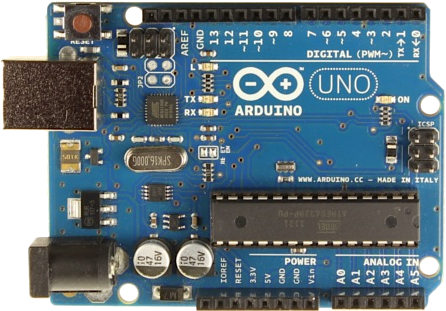
\includegraphics[width=0.4\textwidth]{Bilder/ArduinoUno_Front.png}
\end{flushright}

\vfill {\Large Marie-Curie Gymnasium }\par\vspace*{3\baselineskip} \endgroup}


%% Anhaende
\usepackage{appendix}

\renewcommand{\appendixtocname}{Anhänge}

%% Index 
\usepackage{makeidx}
\makeindex

%% Glossar
\usepackage{glossaries}
\makeglossaries
 
%% section mit neuer Seite anfangen
\let\stdsection\section 
\renewcommand\section{\newpage\stdsection}

\newcommand{\sectionExkurs}[1]{\section{\color{pigment}{#1}}} 
\newcommand{\sectionInformatik}[1]{\section{\color{orange}{#1}}} 
 
%% Kopf- und Fußzeile 
\pagestyle{fancy}
\renewcommand{\chaptermark}[1]%
   {\markboth{\MakeUppercase{\thechapter.\ #1}}{}}
\renewcommand{\sectionmark}[1]{
\markboth{\thesection{} #1}{}
}


%% Hintergrundbild fuer Titelseite
 \newcommand\BackgroundPic{
\put(0,0){
\parbox[b][\paperheight]{\paperwidth}{%
\vfill
\centering
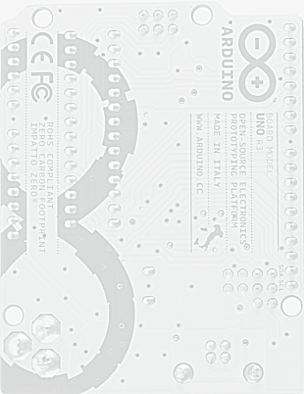
\includegraphics[width=\paperwidth,height=\paperheight,
keepaspectratio,angle=90]{Bilder/background.png}%
\vfill
}}}

%% Eigene Commandos
\newcommand{\ArduinoHomepage}[1]{\href{http://www.arduino.cc/#1}{www.arduino.cc/#1}}


  
\newcommand{\AB}[1]{\textbf{AB} ``\textit{#1}''}

%% begin document %%
\begin{document}
\AddToShipoutPicture*{\BackgroundPic}

\sffamily
\begin{titlepage}
\titleTH



%%  only section used in tableofcontents
\setcounter{tocdepth}{1}
  
\end{titlepage}

\begin{abstract}
\epigraph{If you get, give. If you learn, teach}{Maya Angelou (April 4, 1928 – May 28, 2014),African-American author, poet, dancer, actress and singer}

Arduino is an open-source electronics prototyping platform based on flexible, easy-to-use hardware and software. It's intended for artists, designers, hobbyists, and anyone interested in creating interactive objects or environments.

\end{abstract}

\section*{Impressum}
\begin{flushright}
\today \\
Version 0.5 \\
Wolfgang Wolff \\
Marie-Curie Gymnasium Kirchzarten \\
wolff@mcg-kirchzarten.de
\vfill

\includegraphics[ ]{Bilder/cc}

Dieses Werk bzw. Inhalt steht unter einer Creative Commons Namensnennung-Nicht-kommerziell-Weitergabe unter gleichen Bedingungen 3.0 Unported Lizenz.
\end{flushright}

 % Kapitel 0 % 
\chapter*{Vorwort}
\epigraph{Irrend lernt man.}{Johann Wolfgang von Goethe
(1749 - 1832), deutscher Dichter der Klassik, Naturwissenschaftler und Staatsmann}

Dieses Skript ist nicht fehlerlos. Fehler beschreiben meiner Meinung nach einen Prozess. Wenn man etwas neues lernen möchte, dann sind sie unumgänglich! Deshalb sollte man auch keine Angst davor haben Fehler zu begehen. Solange man bereit ist aus ihnen zu lernen.

In diesem Skript gibt es zwei Arten von Fehlern, einfache Schreibfehler und inhaltliche Fehler. Schreibfehler sind ärgerlich, aber solang der Sinn des Textes nicht verändert wird nicht tragisch. Bei inhaltlichen Fehlern sieht es ganz anders aus. Wenn in einem Beispiel-Sketch ein Fehler ist, dann wird dieser Sketch nicht mehr funktionieren! Wenn in einem Schaltplan zwei PINs vertauscht sind, kann sogar ein elektronisches Bauteil zerstört werden. Solltest du einen Fehler (egal welcher) finden, dann würde ich mich freuen, wenn du ihn mir mitteilen würdest.

Du wirst dich aber auch mit deinen eigenen Fehlern befassen müssen! Wenn du wirklich lernen möchtest, wie ein Mikrocontroller funktioniert und wie du ihn programmierst (wovon ich ausgehe), dann ist es sehr wichtig, dass du alle Aufgaben selber löst! Du wirst Fehler machen, deine Schaltungen werden nicht funktionieren, andere Gruppen werden viel schneller sein! Dies sollte dich nicht entmutigen. Wenn du ehrlich die Aufgaben löst wirst du feststellen, dass ab einem gewissen Punkt du auf einmal viel schneller wirst! Eben wann, wenn du kapiert hast, wie die ganze Sache funktioniert.  

\textbf{Was solltest du tun, wenn du nicht mehr weiter kommst?} Wenn etwas nicht funktioniert, dann Frage deine Mitschüler, deinen Lehrer. Versuche deinen Fehler zu finden und zu verstehen. Es macht keinen Sinn einfach weiterzumachen oder einen richtigen Sketch von der Nachbargruppe zu benutzen! Wichtig ist, dass du alle deine selbst geschriebenen Sketche gut dokumentierst. So schafft du dir selber eine gute Basis auf der du weitere Aufgaben lösen kannst.



\clearpage
\addtocontents{toc}{\protect\setcounter{tocdepth}{1}}
\tableofcontents

\clearpage


%\include{Kapitel0/kapitel0}

 % Kapitel 1 %
\chapter{Einführung}

\epigraph{„Ich denke, dass es einen Weltmarkt für vielleicht fünf Computer gibt.“}{Thomas Watson, IBM-Vorsitzender, 1943}


\label{chapter:1}\chaptermark{Einführung}
Der Arduino ist  eine einfache und vielseitige  Experimentierplattform, eine Art kleiner Mini-Computer. Sie besteht aus der Arduino-Hardware, einer handtellergroßen Platine mit einer Vielzahl von Anschlüssen und der Arduino-Software, einer Entwicklungsumgebung (IDE) für den PC, in der man die Programme schreibt, die auf dem Gerät ablaufen. Das Besondere an dem Arduino-Board ist, dass der Schaltplan freie Hardware (eng. open source hardware) ist. \margininfo{open source hardware ist eine Hardware oder ein sonstiges technisches Gerät, die nach lizenzkostenfreien Bauplänen hergestellt werden.}    

Nach dem du dieses Kapitel gelesen und alle Aufgaben gemacht hast, sollten dir folgende Begriffe bekannt sein.
\begin{itemize}
\item Arduino Board
\item IDE
\item Sketch
\item \textit{setup()} und \textit{loop()}
\end{itemize}


% Kapitel 1

\section{Das Arduino Projekt}

Die Arbeit mit Mikrocontrollern und die Ansteuerung von Hardware hat selbst für Informatiker immer etwas Geheimnisvolles an sich – dafür müsse man wochenlang Datenblätter lesen und dann kryptischen Code schreiben, so die Vorstellung. Aber es geht auch anders! Jedenfalls seit 2005: Da waren es die Studierenden des Interaction Design Institute im italienischen Ivrea leid, mit ihren Computern nur über Tastatur und Maus zu kommunizieren. Sie suchten nach einer einfachen Möglichkeit, um ihre Ideen für neuartige Interaktionen zwischen Mensch und Maschine, ihre Kunst- und Roboterprojekte in funktionsfähige Prototypen umzusetzen. 

Massimo Banzi entwickelte daraufhin mit einer handvoll Mitstreitern ein einfaches, günstiges Mikrocontroller-Board samt Programmiersprache und Entwicklungswerkzeug und nannte es Arduino, nach einem lokalen König aus dem elften Jahrhundert.

Das kleine Entwicklungs-Board trat schnell einen Siegeszug an – gerade weil es sich nicht so sehr an lötende Nerds, sondern an Quereinsteiger wie Designer, Künstler oder auch Schüler richtete, die vorher nur in Ausnahmefällen Software entwickelt oder gar eigene Hardware gebaut hatten. 

\subsection{Was kann man mit dem Arduino alles machen?}

Das Netz ist voller Projekte, die von einer Laserharfe über twitternde Topfpflanzen bis zu autonom fliegenden Luftschiffen reichen.

Ich möchte das Projekt von Zoe Romano: 
\href{http://blog.arduino.cc/2014/07/17/a-low-cost-robotic-hand-tutorial-mirroring-your-own-fingers/}{A low-cost robotic hand (tutorial) mirroring your own fingers} (siehe Video)
genauer anschauen. Ziel dieses Projektes ist es die Bewegungen der Hand zu erfassen und auf eine RoboterHand zu übertragen.

Dieses Projekte besteht aus drei Teilen (siehe Abb. \ref{fig:sla}):
 
\begin{itemize}
  \item Einem Sensor, der Handschuh mit den Biegesensoren, die die Fingerbewegungen messen. 
  \item Einer Logik, das Arduino Board, das die Messwerte verarbeitet und die Bewegung steuert.
  \item Einem Aktor, der RoboterHand, die die Bewegungen ausführt. 
\end{itemize}
Diese Projekt ist ein gutes Beispiel für die Arbeitsweise eines Mikrocontrollers. Ein Mikrocontroller kann über Sensoren Daten einlesen  (Eingabe), diese Daten verarbeiten (Verarbeiten) und Aktoren (LEDs, Motoren, Lautsprecher, \dots) steuern (Ausgabe).   
\margininfo{Eingabe, Verarbeiten und Ausgabe: das EVA-Prinzip}

Genau wie dieses Projekt ist auch dieses Skript aufgebaut. Im ersten Kapitel erfährt du einiges über die Funktionsweise des Arduino-Boards. In Kapitel 2 wirst du mit verschiedenen Sensoren arbeiten und in Kapitel 3 wird schließlich die Funktionsweise verschiedener Aktoren thematisiert.
 
\begin{figure}[h]
\begin{center}
  \begin{tikzpicture}[remember picture]
    % Image 
    \node[anchor=south west,inner sep=0] (image) at (0,0) {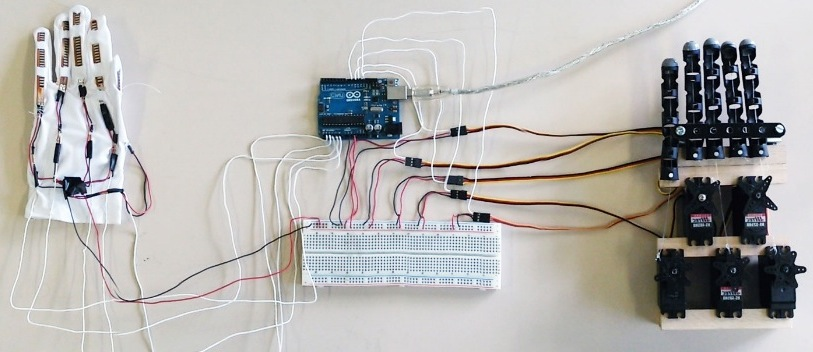
\includegraphics[width=0.9\textwidth]{Kapitel1/Bilder/roboticHand}};
    % Marks 
    \draw[very thick, color=red,rounded corners=0.3cm] (0,1)  rectangle (3.5,7.5) node (sensor) at (1.75,1) {};
    \draw[very thick, color=red,rounded corners=0.3cm] (6,4)  rectangle (9,6.5) node (arduino) at (7.5,4) {};
    \draw[very thick, color=red,rounded corners=0.3cm] (13.5,0)  rectangle (17.5,7) node (actor) at (15.5,0) {};
    % comment
    \node[draw=red, fill=red!20, rounded corners,minimum width=0.2\textwidth, minimum height=1.4\baselineskip, anchor=west,align=center,text width=0.2\textwidth] (item1) at (0,-1) {Sensor: SenorHandschuh};
    \node[draw=red, fill=red!20, rounded corners,minimum width=0.2\textwidth, minimum height=1.4\baselineskip, anchor=west,align=center,text width=0.2\textwidth] (item2) at (6,-1){Logik: ArduinoBoard};
    \node[draw=red, fill=red!20, rounded corners,minimum width=0.2\textwidth, minimum height=1.4\baselineskip, anchor=west,align=center,text width=0.2\textwidth] (item3) at (13.5,-1){Aktor: RoboterHand};
    % grid 
  %\draw[color=red,help lines,xstep=1,ystep=1] (0,0) grid (18,8);
  %\draw[help lines,thin,xstep=.5,ystep=.5] (0,0) grid (18,8);
  %\foreach \x in {0,1,...,18} { \node [anchor=north] at (\x,0) {\x}; }
  %\foreach \y in {0,1,...,8} { \node [anchor=east] at (0,\y) {\y}; }  
  \path[red, thick,-] (sensor.south) edge [out=-90 , in=90] (item1);
  \path[red, thick,-] (arduino.east) edge [out=-90 , in=90] (item2);
  \path[red, thick,-] (actor.east) edge [out=-90 , in=90] (item3);
  \end{tikzpicture}
  \end{center}
  \caption{Aufbau eines Arduino-Projektes}
  \label{fig:sla}
\end{figure}

\subsection{Projekte und Ideen, die ohne Arduino wirklich schwer währen!}

Bevor du dich ausführlich mit dem Arduino Uno beschäftigst, möchte ich dir eine kurze Auswahl verschiedener Projekte vorstellen

\subsubsection{Manufaktur -- Arduino als Maker }

Werkstücke mit Hilfe eines PC fertigen, war bis vor kurzer Zeit nur mit sehr teuren CNC-Maschinen und teurer Spezialsoftware möglich.
\margininfo{CNC (Computerized Numerical Control) Computergestützte numerische Steuerung} 
Durch die Entwicklung des Arduino-Projekts (und anderer ähnlicher Projekte) wurde es möglich CNC-Maschinen und 3D-Drucker viel billiger zu bauen. Natürlich sind diese selbstgebauten Maschinen nicht mit industriellen Maschinen vergleichbar, dafür sind die aber um den Faktor 100-1000 billiger und somit in Bereichen einsatzbar die zuvor finanziell nicht möglich waren.
   
Zwei dieser Projekte möchte ich herausheben:
\begin{itemize}
  \item \href{http://www.shapeoko.com/}{Shapeoko An Open Hardware project by Edward Ford}
  \item \href{http://www.open-electronics.org/3drag-the-open-electronics-way-to-reprap/}{3Drag: the Open Electronics way to RepRap}
\end{itemize}
\begin{figure}[h]
  \begin{center}
    \subfigure[Shapeoko open hardware CNC-Fräse]{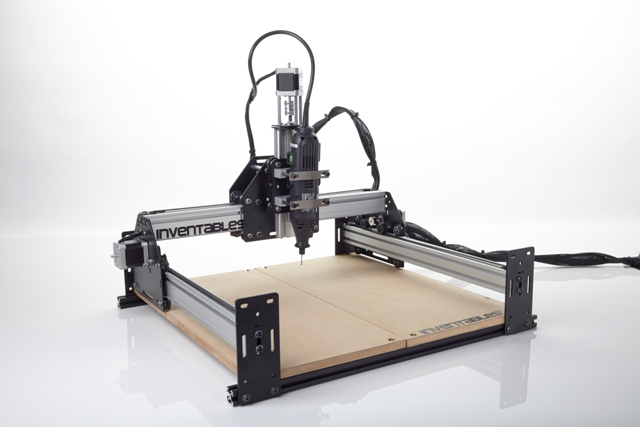
\includegraphics[width=0.5\textwidth]{Kapitel1/Bilder/Shapeoko.jpg}}
    \subfigure[3Drag open electronic 3D-Drucker]{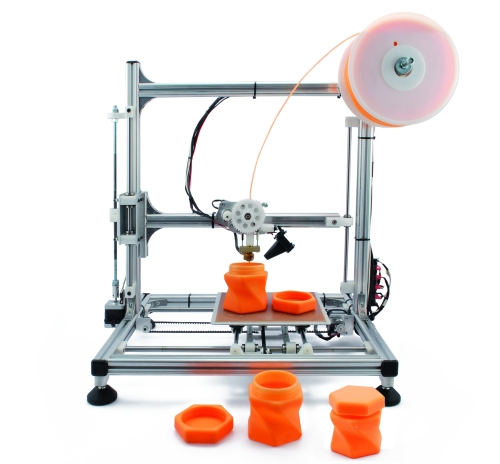
\includegraphics[width=0.4\textwidth]{Kapitel1/Bilder/RepRap.jpg}}
    \label{fig:Manufaktur}
    \caption{Manufaktur: Arduino steuert CNC-Maschinen}
  \end{center}
\end{figure}


\subsection{Art und Design -- Arduino als Künstler}

Das Arduino-Board  wurde ursprünglich für die universitäre Ausbildung zum „Interaction Designer“ entwickelt. Die Motivation liegt darin Elektronik als kreatives Material einzusetzen. So kann mit Hilfe eines LED-Cubes (siehe Abb. \ref{fig:cube}) Musik als fallende Tropfen oder Silvesterraketen dargestellt werden. 

Mit einem Arduino LilyPad können intelligente Kleidungsstücke designed werden. Zum Beispiel eine Tasche, mit steuerbaren LEDs (siehe Abb. \ref{fig:bekathwia}).

\begin{itemize}
  \item \href{https://www.youtube.com/watch?v=6mXM-oGggrM}{LED cube 8x8x8 demo by chrmoe}
  \item \href{http://www.instructables.com/id/LilyPad-Arduino-Blinking-Bike-Safety-Patch/}{LilyPad Arduino Blinking Bike Safety Patch
by bekathwia}
\end{itemize}

\marginfigure{Kapitel1/Bilder/lillipad}{Arduino LilyPad}{fig:lillipad} 


\begin{figure}[h]
  \subfigure[LED Cube 8x8x8 by chr\label{fig:cube}]{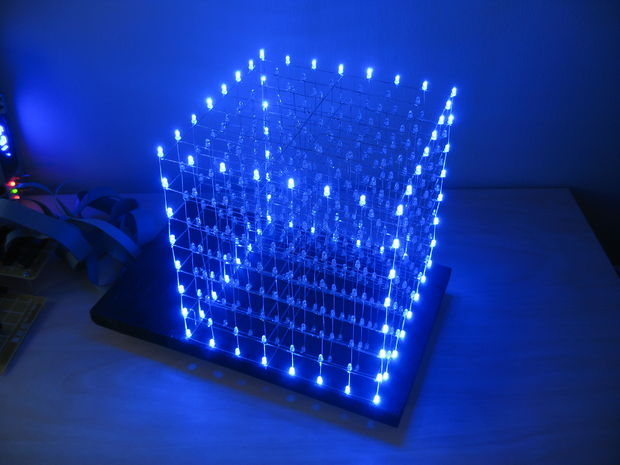
\includegraphics[width=0.38\textwidth]{Kapitel1/Bilder/cube-7x7x7}}\qquad
  \subfigure[LilyPad Arduino Blinking Bike Safety Patch
by bekathwia  (by-nc-sa)\label{fig:bekathwia}]{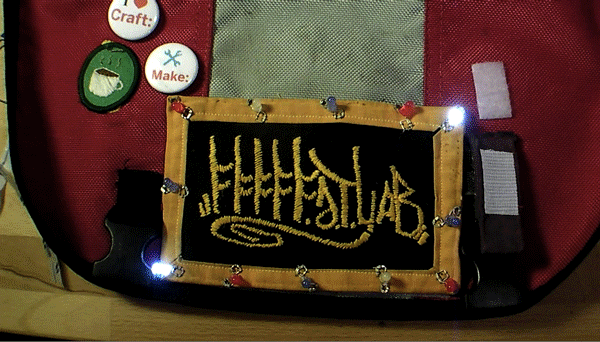
\includegraphics[width=0.5\textwidth]{Kapitel1/Bilder/lillipad-proj}}
  \label{fig:Art}
  \caption{Art: Arduino als Künstler}
\end{figure}

%\subsection{Schuleprojekte mit dem Arduino}
%
%\begin{figure}[h]
%   \subfigure[Roboter Auto (Unterrichtsprojekt Klasse 9)]{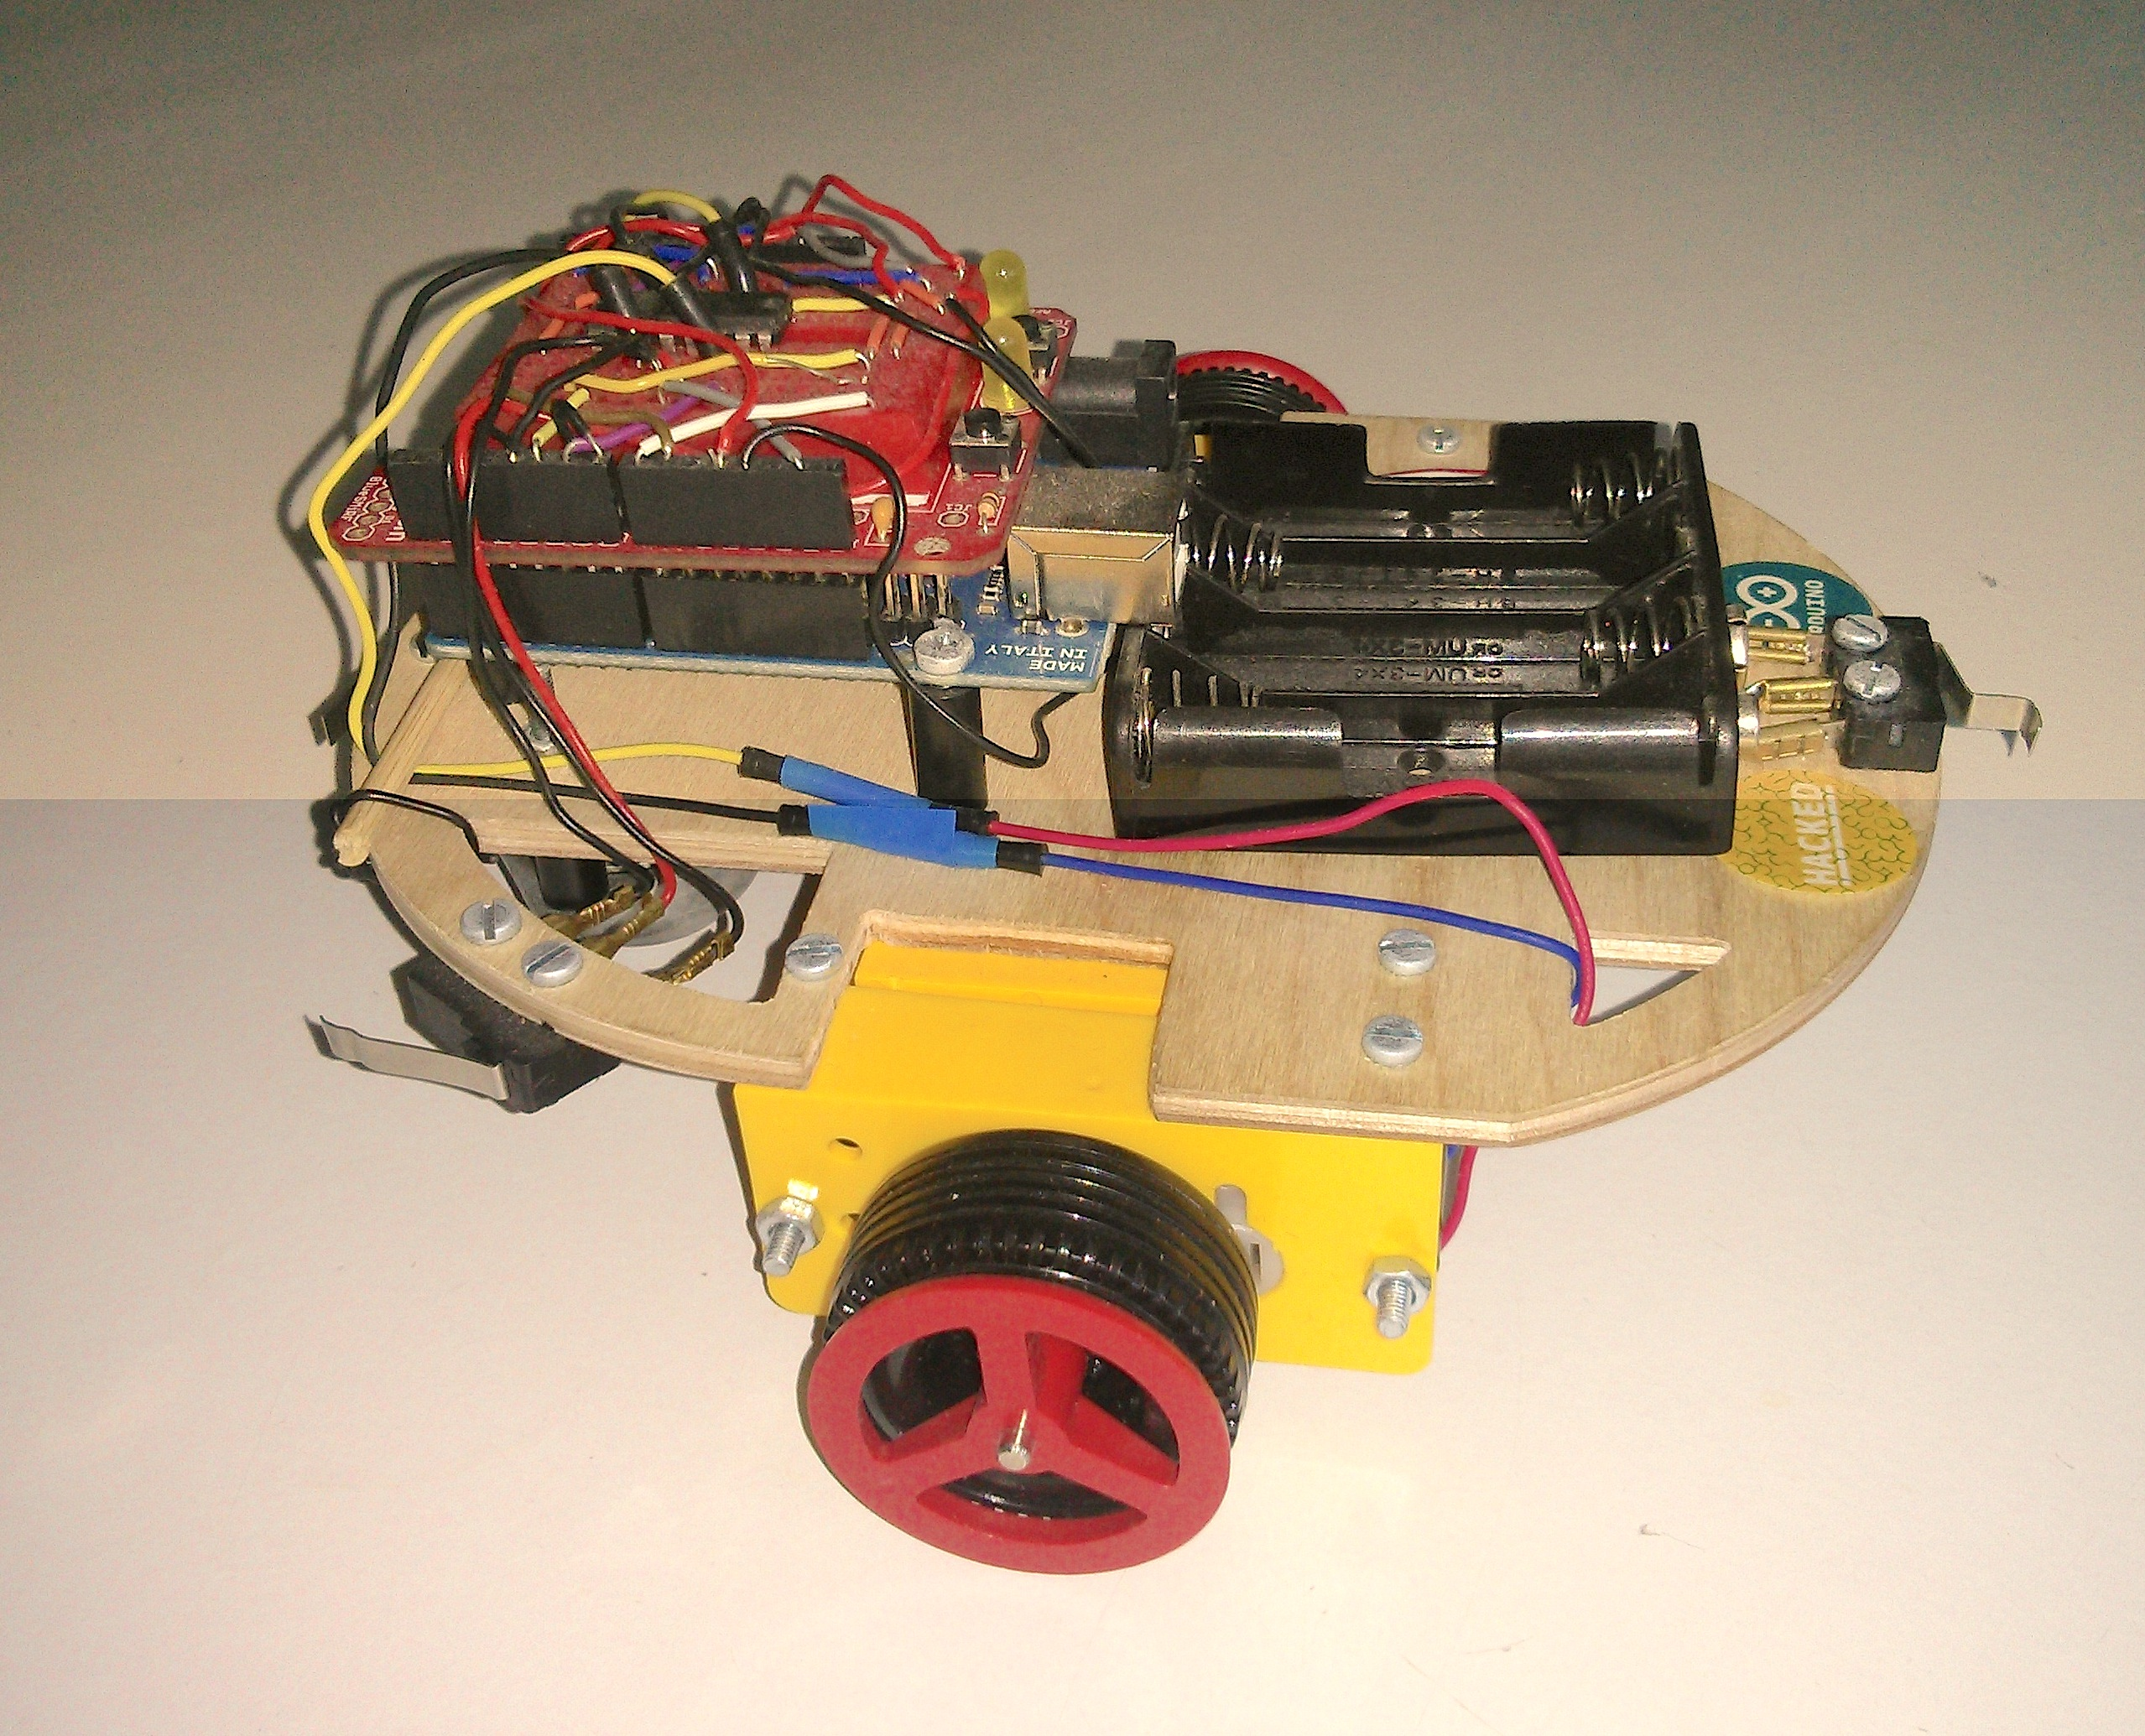
\includegraphics[width=0.35\textwidth]{Kapitel1/Bilder/robocar}}
%  \label{fig:Art}
%  \caption{Art: Arduino als Künstler}
%\end{figure}

\subsection{Der Mikrocontroller}

Der Kern eines Arduino ist der Mikrocontroller. Ein Mikrocontroller ist aus miniaturisierten elektrischen  Schaltkreisen -- den integrierten Schaltkreisen aufgebaut. 
\marginfigure{Kapitel1/Bilder/ATmega328}{Der ATmega328-Mikrocontroller (CC BY-NC-SA 3.0 by sparkfun.com)}{fig:ATmega328}

ICs sind komplexe elektrische Schaltungen, die auf kleinstem Raum in einem Siliziumkristall platz finden.
Was zu den Pionierzeiten der Elektronik noch mit unzähligen Bauteilen (Dioden, Transistoren, Widerständen und Kondensatoren) platzraubend Aufgebaut werden musste, findet heute auf kleinstem Raum platz in unterschiedlich großem schwarzen Plastikgehäusen mit einer bestimmten Anzahl von Beinchen, den sogenannten PINs. 
\margininfo{IC - Integrated Circuit} 

In der Abb. \ref{fig:ATmega328} siehst du den ATmega328-Mikrocontroller, der auch auf dem
Arduino Uno Board verbaut ist.  Du könntest ihn in dieser Form mit Hilfe einer geeigneten Spannungsversorgung und einem Taktgebers benutzten. Leider ist das aber sehr kompliziert. Aus diesem Grund wird der IC auf dem Arduino Uno Board montiert. Aufgabe dieses Entwicklungs-Boards ist es dir die Welt der Mikrocontroller auf möglichst einfache Weise zugänglich zu machen.

\subsubsection{Der innere Aufbau eines $\mu$Cs}

Der Aufbau eines Mikrocontrollers entspricht dessen eines Computers. Der Unterschied besetzt in der Leistungsfähigkeit, der Rechenleistung und im Speichervolumen.   

In der Abb. \ref{fig:blockdiagramm_yc} sind die Bestandteile eines ATmega schematisch dargestellt.

\marginfigure{Kapitel1/Tikz/blockdiagramm}{Blockdiagramm}{fig:blockdiagramm_yc} 

\begin{itemize}
  \item \textbf{Die CPU}  steuert und kontrolliert die anderen Teile des Mikrocontrollers durch dekodieren und ausführen von (Maschinen-)Befehlen. Sie kann den Speicher adressieren, Ein- bzw. Ausgänge verwalten und auf sogenannte Interrupts reagieren. 
  \item \textbf{Der Datenbus} verbindet alle Bestandteile des Mikrocontrollers miteinander. Die CPU fordert zum Beispiel Daten aus dem Speicher an, die Daten werden auf den Bus gelegt und können unmittelbar von der CPU verarbeitet werde.
  \item \textbf{Die Interrupt Steuerung (IRW)} kann auf  stattfindende Ereignisse reagieren. Dazu wird die aktuelle Aufgabe unterbrochen um sofort auf das Ereignis  reagieren zu können. 
  \item \textbf{Speicher RAM und ROM} (siehe Aufgabe)
\end{itemize}  

\subsection{Aufgabe:}

Was ist eigentlich der Unterschied zwischen RAM und ROM Speicher. Liese den Artikel \url{http://de.ccm.net/faq/3349-der-unterschied-zwischen-ram-und-rom} und erkläre die jeweilige Funktion ein eigenen Wörtern. 



\clearpage
\section{Das Arduino Uno Board}

Hier ist die neuste Version der Arduino-Hardware (Stand: März 2012) abgebildet, der Arduino 
Uno (R3)\index{Arduino Uno}. Die wichtigsten Anschlüsse und Bestandteile sind die folgenden:
\marginfigure{Kapitel1/Bilder/arduinouno}{Arduino Uno R3}{fig:arduinouno}
\begin{itemize}
\item[\textcolor{red}{A}] \textbf{Der Mikrocontroller} ist das wichtigste Bauteil des Arduinos. Beim Arduino Uno ist ein Atmel ATmega328 verbaut. 


\item[\textcolor{red}{B}] 
Über den \textbf{USB-Anschluss} verbindet man den Arduino mit dem PC. Über diese Verbindung überträgt man den Programmcode, das der Arduino ausführen soll, in den ROM Speicher des Mikrochips. Während das Programm ausgeführt wird, kann außerdem Daten zwischen PC und Arduino austauscht werden.

\item[\textcolor{red}{C}] 
Die rechte Buchsenleiste besteht aus 14 \textbf{digitalen Ein-} oder \textbf{Ausgängen}, sogenannten digitalen PINs. Ein digitaler PIN kann mit Hilfe eines Schalters oder Temperatur-Sensors Daten empfangen oder mit Hilfe eines Lautsprecher, einer Leuchtdiode oder einem anderem Bauteile Daten aussenden. Digital bedeutet, dass an den digitalen PINs entweder $0\V$ (digital 0/LOW) oder $5\V$ (digital 1/HIGH) Spannung anliegt. Ein digitaler PIN kann maximal 40mA Strom liefern.

Sechs digitale PINs besitzen noch die Zusatzfunktion der \textbf{PWM} (Pulsbreitenmodulation) \margininfo{PWM für pulse width modulation}. Diese PINs sind zusätzlich mit einer  \~  gekennzeichnet. 

\item[\textcolor{red}{D}] Der untere Teil der linken Buchsenleiste ist mit \textbf{Analog in} beschriftet. Mit Hilfe der analogen PINs können Spannungen zwischen 0V und 5V gemessen werden.

\item[\textcolor{red}{E}] 
die linke obere Buchsenleiste trägt die Bezeichnung \textbf{Power}:
   ``Vin'' (Voltage in) Eingangsspannung, ``Gnd'' (Ground)  0 Volt, ``5V'' (5 Volt), ``3V3'' (3,3 Volt), ``Reset''
\end{itemize}
Es gibt noch weitere Bauteile: Stromversorgung, Reset-Taster, Status-LEDs, Kondensatoren, Widerstände und einen Quarz.
 
\subsection{Aufgaben}

\subsubsection{Aufgabe 1:} 
Im PDF-File \href{http://marcusjenkins.com/wp-content/uploads/2014/06/ARDUINO_V2.pdf}{Arduino Uno V3 Pinout Diagram} ist der Aufbau des Arduino Uno nochmals sehr genau erklärt. Suche und kennzeichne alle GND-PINs, den Reset-Taster.    


\section{Software: die Arduino-IDE}

Die Arduino Entwicklungsumgebung\index{IDE} ist für Linux, OS X und Windows kostenlos verfügbar und kann von der Arduino Homepage heruntergelagen werden: \href{https://www.arduino.cc/en/Main/Software}{Download the Arduino Software}.

Die Entwicklungsumgebung besteht aus folgenden Teilen
\begin{itemize}
  \item[\textcolor{red}{A}]  den Menüs
  \item[\textcolor{red}{B}]  Texteditor zum schreiben des Programm-Codes
  \item[\textcolor{red}{C}]  einer Nachrichtenkonsole
\end{itemize}

Die Entwicklungsumgebung stellt automatisch eine Verbindung zur Arduino Hardware her um Programme hochzuladen und um weiter Daten mit dem Arduino auszutauschen. Ein fertiges Programme  wird ``Sketch'' genannt. Ein ``Sketch'' wird mit einem Text-Editor geschrieben und automatisch mit der Dateiendung ``.ino'' gespeichert. Jeder Sketch wird automatische in einem Eigenen Ordner gespeichert. Der Nachrichtenbereich gibt Feedback beim Speichern und Exportieren von Sketchen und eventuell auftretenden  Fehlern. 

\marginfigure{Kapitel1/Bilder/ide}{Die Arduino IDE (Version 1.0)}{fig:ide}

Die Bedeutung der Icons in der Symbolleiste \textcolor{red}{A} sind:
\begin{itemize}
  \item[] 
\includegraphics[width=0.03\textwidth]{Kapitel1/Bilder/verify} \textbf{Verify}:  Überprüft deinen Code auf syntaktische Fehler.
  \item[]  
\includegraphics[width=0.03\textwidth]{Kapitel1/Bilder/play} \textbf{Play}: Kompiliert deinen Programmcode und lädt ihn auf das Arduino Board.
  \item[] 
\includegraphics[width=0.03\textwidth]{Kapitel1/Bilder/new} \textbf{New}: Erschafft einen neuen ``sketch''.
  \item[]  
\includegraphics[width=0.03\textwidth]{Kapitel1/Bilder/open}   \textbf{Open}: Öffnet ein Menu mit allen Sketchen, die auf dem PC (deine eigenen Sketche und Beispiel-Sketche) gespeichert sind. Durch anklicken kannst du einen Sketch öffnen.
  \item[] 
\includegraphics[width=0.03\textwidth]{Kapitel1/Bilder/save} \textbf{Save}: Speichert deinen ``sketch''.
  \item[] 
\includegraphics[width=0.03\textwidth]{Kapitel1/Bilder/serial_monitor} \textbf{Serial Monitor}: öffnet ein Konsole, die über die USB-Schnittstelle eine serielle Verbindung zum Arduino aufbaut. 
\end{itemize}

\subsection{Aufgaben}

Starte die Arduino IDE. Verbinde mit dem UBS-Kabel dein Arduino Uno Board mit dem PC. Schaue im Menu ``Werkzeuge - Port'' nach, ob dein Arduino verbunden ist. Wenn dein Arduino richtig verbunden ist, dann kannst du ebenfalls im Menu ``Werkzeuge'' den ``Serieller Plotter'' öffnen. Erkläre die Funktion des Serieller Plotter's.  


\section{Blink, dein erster Arduino Sketch}\label{sec:blink}

\subsubsection{Vorbemerkungen}
Im ersten Teil dieser Einführung wirst du eine Ampelanlage mit Auto- und Fußgängerampel aufbauen und programmieren. Die benötigte Schaltung und den Sketch wirst du in den folgenden Abschnitten Stück für Stück erarbeiten. Es ist deshalb wichtig, dass du die jeweiligen Schaltpläne möglichst genau aufbaust. So sparst du Zeit, da du deine Schaltung nicht umbauen musst. 

\begin{figure}[h]
  \begin{center}
  \subfigure[Schaltplan]{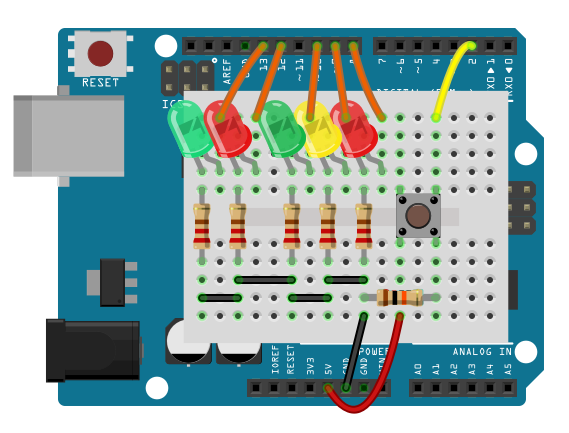
\includegraphics[width=0.45\textwidth]{Kapitel1/Bilder/ampelFertig}}
  \subfigure[Reale Schaltung]{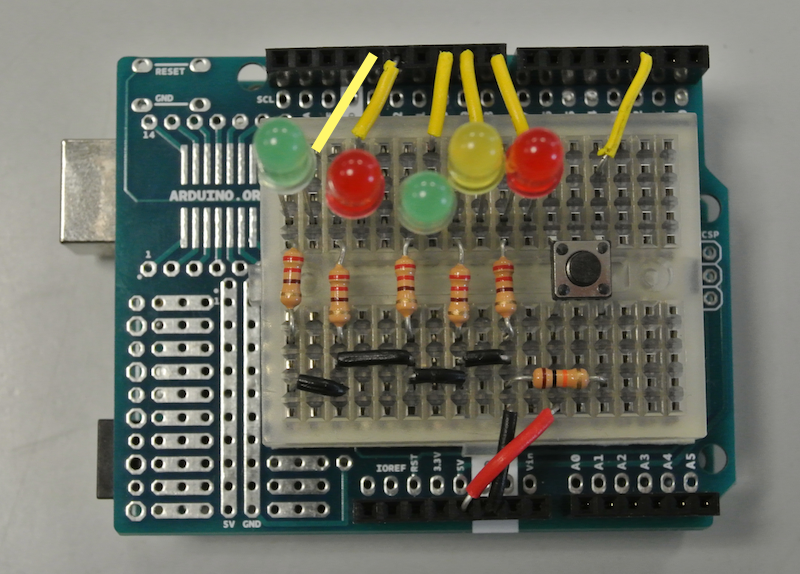
\includegraphics[width=0.45\textwidth]{Kapitel1/Bilder/ampelFertigReal}}
  \label{fig:ample}
  \caption{Die fertige Ampel}
  \end{center}
\end{figure}
  
\clearpage

\subsubsection{Jetzt geht es los!}

Um deinen ersten Arduino Sketch auf den Arduino zu übertragen und auszuführen musst du folgende Schritte nacheinander ausführen:

\marginfigure{Kapitel1/Bilder/arduino_blink_2}{Öffnen eines Sketches}{fig:blink2}

\begin{itemize}
  \item[1.] Starte die Arduino IDE und öffne das Beispiel ``Blink'' (siehe Abb. \ref{fig:blink2}).
  \item[2.] Verbinde nun das Arduino-Board und deinen PC mit Hilfe des UBS-Kabels.
  \item[3.] Drücke in der Arduino-IDE das Icon 
\includegraphics[width=0.03\textwidth]{Kapitel1/Bilder/play} um den Sketch zu übersetzen, auf den Arduino zu übertragen und um das Arduino-Programm auszuführen.
\end{itemize}

Jetzt sollte die kleine LED mit der Beschriftung ``L'' periodisch blinken.

\subsection{Eine externe LED blinken lassen}

Es kann auch eine ``externe'' LED zum Leuchten gebracht werden. Am schnellsten geht das, wenn man die LED direkt auf dem Arduino-Board in den ditigalen  Anschluß PIN13 und den daneben liegenden Anschluß GND steckt (siehe Abb. \ref{fig:arduino_blink_schaltung}). Sollte die LED von PIN13 blinken aber die externe LED nicht so hast du die LED falsch herum angeschlossen. 

\marginfigure{Kapitel1/Bilder/LEDmitWiderstand}{LED und Vorwiderstand}{fig:LEDmitWiderstand}

\margininfo{Achtung verbinde nie eine LED mit dem PIN Vin. Je nach Versorgungspannung wird die LED explosionsartig zerstört!}

\begin{figure}[h]
  \begin{center}
    \subfigure[Schnelle Methode]{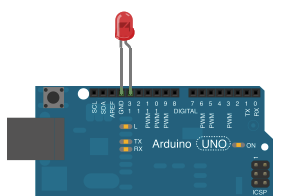
\includegraphics[width=0.3\textwidth]{Kapitel1/Bilder/arduino_blink_schaltung}
      \label{fig:arduino_blink_schaltung_schnell}}
    \subfigure[LED mit Vorwiderstand an PIN 10]{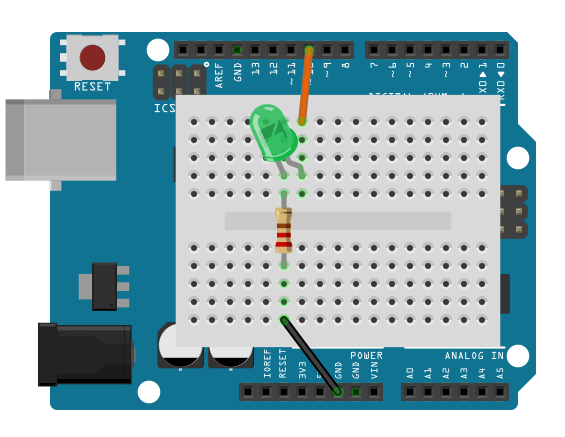
\includegraphics[width=0.3\textwidth]{Kapitel1/Bilder/ampelG}
      \label{fig:arduino_blink_schaltung_vorwiderstand}}
    \caption{Anschluss einer externen LED}
    \label{fig:arduino_blink_schaltung}
  \end{center}
\end{figure}


Die schnelle Methode sollte nur zum Testen verwendet werden, da die LED kaputt gehen kann. Deshalb sollte eine LED immer zusammen mit einem Vorwiderstand betrieben werden (siehe Abb. \ref{fig:arduino_blink_schaltung_vorwiderstand}). Die Funktion des Vorwiderstandes ist es, die maximale Leistungsaufnahme der LED zu begrenzen. Für eine normale LED ist ein Vorwiderstand von $R=220\Ohm$ ausreichend. Mehr Wissen zum Thema Elektronik findest du im Anhang \ref{ch:anhang_elektronik} Hintergrundwissen Elektronik.

\subsubsection{Farb-Code von Widerständen} 

Wenn du die Abbildung \ref{fig:LEDmitWiderstand} den Widerstand genauer ansiehst, dann erkennst du die vier farbigen Ringe, die ersten drei Ringe ergeben den Widerstandswert, der vierte Ring die Fertigungstoleranz an. Es gibt viele Internetseiten, auf denen du die Farbcodes nachschauen kannst. Mein persönlicher Favorit ist die Seite \url{http://resisto.rs}. 

\marginimage{Kapitel1/Bilder/resistor_rs}


\clearpage
\subsection{Ein kurzer Blick auf den Sketch-Code} 

Der Arduino wird in der Computersprache C programmiert. C ist zwar alt, aber immer noch eine der beliebten  Programmiersprachen.
Schau dir den Programm-Code des Sketches ``Blink'' (siehe Listing \ref{lst:blink}) einmal genauer an. 

\begin{multicols}{2}
\begin{arduinoCode}{Blink}{lst:blink}
/*  (*@ \label{lis:blink_beginkommentar} @*) 
  Blink
  Turns on an LED for one second, then off for one second, repeatedly. 
                       (*@ \tikzmark{comment} @*)
  This example code is in the public domain.
*/ (*@ \label{lis:blink_endkommentar} @*)

void setup() {       (*@ \tikzmark{setup} @*)       
  // initialize the digital pin as an output.
  // PIN 13 has an LED connected on most Arduino boards:
  pinMode(13, OUTPUT);   (*@ \tikzmark{pinMode} @*)   
}   (*@ \label{lis:blink_endsetup} @*)   

void loop() { (*@ \label{lis:blink_beginloop} @*)         
  digitalWrite(13, HIGH);   (*@ \tikzmark{ledHigh} @*)
  // set the LED on
  delay(1000);    // wait for a second
  digitalWrite(13, LOW);    (*@ \tikzmark{ledLow} @*)
  // set the LED off
  delay(1000);    // wait for a second
} (*@ \label{lis:blink_endloop} @*)      
\end{arduinoCode}

\vfill
\columnbreak

\null\vfill
\begin{itemize}
  \itemsep45pt
  \item[] \tikzmarkcomment{item1}{Kommentarbereich: Hier wird die Aufgabe, Funktionsweise und weiter wichtige Informationen dokumentiert.}
  \item[] \tikzmarkcomment{item2}{Die setup()-Methode wird nur einmal ausgeführt}
  \item[] \tikzmarkcomment{item3}{PIN13 wird als  OUTPUT definiert.}
  \item[] \tikzmarkcomment{item4}{Die loop()-Methode wird immer wieder ausgeführt. Dadurch wird die LED für eine Sekunde (1000ms) eingeschalten und ...}
  \item[] \tikzmarkcomment{item5}{... anschließend ausgeschaltet. Nach einer weiteren Sekunde wiederholt sich das EInschalten.}
\end{itemize}
\vfill \null

\begin{tikzpicture}[remember picture,overlay]
  \path[red, thick,-] (comment.east) edge [out=0 , in=180] (item1);
  \path[red, thick,-] (setup.east) edge [out=0 , in=180] (item2);
  \path[red, thick,-] (pinMode.east) edge [out=0 , in=180] (item3);
  \path[red, thick,-] (ledHigh.east) edge [out=0 , in=180] (item4);
  \path[red, thick,-] (ledLow.east) edge [out=0 , in=180] (item5);
\end{tikzpicture}

\end{multicols}





\subsection{Die bisher verwendeten C Befehle}

In dem Sketch ``Blink'' werden unterschiedliche Strukturen der Programmiersprache C verwendet. Auf der Arduino Homepage
findest du unter \ArduinoHomepage{en/Reference/HomePage} alle C Sprachelemente, die du für die Programmierung eines Arduino nötig sind.

\margininfo{C wurde vom Informatiker Dennis Ritchie in den frühen 1970er Jahren an den Bell Laboratories für die Systemprogrammierung des Betriebssystems Unix entwickelte.}

Die Tabelle \ref{tab:blink_befehle} listet die bisher verwendeten Befehle auf und beschreibt kurz ihre Funktion. 
\begin{table}[h]
\begin{center}
  \tikzset{ 
    table/.style={
        matrix of nodes,
        row sep=-\pgflinewidth,
        column sep=-\pgflinewidth,
        nodes={
            rectangle,
            draw=black,text width=0.75\textwidth,
            align=center
        },
        minimum height=1.5em,
        text depth=0.5ex,
        text height=2ex,
        nodes in empty cells,
%%
        every even row/.style={
            nodes={fill=gray!20}
        },
        column 1/.style={
            nodes={text width=0.25\textwidth}
        },
        column 2/.style={
            nodes={text width=0.75\textwidth}
        },
        row 1/.style={
            nodes={
                fill=black!80,
                text=white,
                font=\bfseries
            }
        }
      }
  }
  \begin{tikzpicture}
  \matrix (first) [table,text width=6em]
  {   
 Name & Funktion \\
  \href{http://arduino.cc/en/Reference/PinMode}{pinMode(PIN, MODE)} & Konfiguriert den angegebenen PIN als 
 INPUT oder OUTPUT.  \\
 \href{http://arduino.cc/en/Reference/DigitalWrite}{digitalWrite(PIN, VALUE)} & Schreibt den VALUE mit einem Wert HIGH oder LOW auf den digitalen PIN.\\
 \href{http://arduino.cc/en/Reference/Delay}{delay(MS) } & Stoppt das Programm für MS Millisekunden. 1000ms entspricht einer Sekunde.\\};
\end{tikzpicture}
\end{center}
\caption{Übersicht der verwendeten C Befehle}
\label{tab:blink_befehle}
\end{table}%

\subsection{Aufgaben}

\subsubsection{Aufgabe 1}

\begin{description}
  \item[a)] Erstelle eine Tabelle, in der du alle C Sprache-Elemente und Strukturen dokumentierst. Orientiere dich an dem Aufbau der Tabelle  \ref{tab:blink_befehle}.   
  \item[b)] Lies auf \ArduinoHomepage{Reference/HomePage} die ausführliche englische Dokumentation der folgenden Befehlen
  \begin{enumerate}
    \item pinMode()  (\ArduinoHomepage{en/Reference/PinMode})
    \item digitalWrite()  (\ArduinoHomepage{en/Reference/DigitalWrite})
    \item delay()  (\ArduinoHomepage{en/Reference/delay})
  \end{enumerate} 
  Gibt es zusätzliche Informationen, die für dich wichtig sein können. Beantworte folgende Fragen schriftlich:
  \begin{itemize}
    \item Was passiert, wenn du einen digitalen PIN zum Steuern einer LED mit pinMode() auf INPUT setzt?
    \item Gibt es für digitale PIN noch weiter Modi?  
    \item Gibt es noch mehre delay()-artige Befehle? Eine Millisekunde ist zwar für einen Menschen eine unheimlich kurze Zeitspanne, für einen Arduino aber schon ziemlich lange!   
  \end{itemize}
  Ergänze deine Tabelle entsprechend.
  \item[c)]Verändere den Sketch ``Blink'' so, dass eine LED am PIN 10 SOS\footnote{Im Morse Alphabet: 
    3 mal kurz (für S) 3 mal lang (für `O') 3 mal kurz (für `S') gefolgt von einer langen Pause und dann wieder vor 
    vorne} blinkt. Den Schaltplan findest du in Abb. \ref{fig:arduino_blink_schaltung_vorwiderstand} 
    Speichere den veränderten Sketch unter dem Namen ``SOS'' ab.
  \item[d)] Erweitere deine Tabelle  mit der Befehlsübersicht um  den folgenden Befehl: 
  \begin{enumerate}
    \item random()  (\ArduinoHomepage{en/Reference/Random}).
  \end{enumerate}
  ein.
  \item[d)] Erstelle den neuen Sketch ``RandomBlink''. Die LED soll an PIN13 nun zufällig an- und ausgehen. 
  Dazu musst du in der loop()-Routine folgenden Befehl ergänzen ``delay(random(2000))''.  
\end{description}
\marginfigure{Kapitel1/Bilder/ampelGYR}{LEDs an PINs 10, 9 und 8}{fig:ampelGYR}

\subsubsection{Aufgabe 2: Steuern einer Autoampel}

Schließe an die digitalen PINs 10, 9 und 8 je eine grüne, gelbe und rote LED mit Vorwiderstand an. Die Schaltung findest du in Abb. \ref{fig:ampelGYR}. Erstelle den neuen Sketch `Ampel', der die 3 LEDs in der Lichtfolge einer Ampel leuchten lässt. Zuerst soll die gründe LED leuchten, achte dann auf die richtige Reihenfolge!


\section{Der Arduino Sketch}

Ein Arduino Sketch besteht aus mehreren  Bereichen:

\begin{itemize}
\item dem Kommentarbereich zur Dokumentation und Funktionsweise des Arduino Sketches. Ein ausführlicher Kommentarbereich hilft dir und anderen deinen Sketch zu verstehen. Du wirst oft auf deine selbst erstellten Sketche zurückgreifen.   
\item dem Definitionsbereich von Variablen 
  und Libraries
\item dem Mothodenbereich, mit der setup()-Methode, die einmal ausgeführt wird und der loop()-Methode, die immer wieder ausgeführt wird. Zusätzlich können noch weitere Methoden dazukommen (dazu aber später mehr). setup()- und loop()-Methode müssen in jedem Sketch vorhanden sein. 
\end{itemize}

\margininfo{Aus Platzgründen wir im folgendem der Kommentarbereich bei den Beispiel-Sketchen immer weggelassen. Du solltest aber bei jedem deiner Sketche einen ausführlichen Kommentarbereich schreiben.}
\begin{multicols}{2}
\begin{arduinoCode}{Bare Minimum}{lst:minimum}
/*        
  Sketch Name und Beschreibung 
  
  Datum:        (*@ \tikzmark{comment} @*) 
  Author:
  Version:
*/

// Definition von Variablen  (*@ \tikzmark{def} @*) 

void setup() {  (*@ \tikzmark{setup} @*)         
      
}

void loop() {   (*@ \tikzmark{loop} @*)         

}

\end{arduinoCode}

\vfill
\columnbreak

\null\vfill
\begin{itemize}
  \itemsep15pt
  \item[] \tikzmarkcomment{item1}{Kommentarbereich}
  \item[] \tikzmarkcomment{item2}{Definitionsbereich \\
  Z.B.: int ledPin = 13;}
  \item[] \tikzmarkcomment{item3}{setup()-Methode}
  \item[] \tikzmarkcomment{item4}{loop()-Methode}
\end{itemize}
\vfill \null

\begin{tikzpicture}[remember picture,overlay]
  \path[red, thick,-] (comment.east) edge [out=0 , in=180] (item1);
  \path[red, thick,-] (def.east) edge [out=0 , in=180] (item2);
  \path[red, thick,-] (setup.east) edge [out=0 , in=180] (item3);
  \path[red, thick,-] (loop.east) edge [out=0 , in=180] (item4);
\end{tikzpicture}

\end{multicols}



\subsection{Aufgaben}

\subsubsection{Aufgabe 1}
Dokumentiere die beiden Sketche ``SOS'' und ``Ampel''.

\section{Mit dem PC kommunizieren}\label{sec:kommunikation}

Bisher hast du, oder besser die ArduinoIDE mit dem Arduino ``gesprochen''. Jedes mal, wenn du einen Sketch auf das Board geladen hast. Natürlich kann man auch direkt mit dem Arduino sprechen. Dies geschieht über eine sogenannte Serielle Schnittstelle. Um zu verstehen wie das funktioniert, öffnest du den Beispielsketch ``DigitalReadSerial'' (siehe Abb. \ref{fig:digitalreadserial}).

\marginfigure{Kapitel1/Bilder/arduino_digitalreadserial}{``DigitalReadSerial'' öffnen}{fig:digitalreadserial}

Der Beispielsketch `DigitalReadSerial' ist in Listing \ref{lst:digitalreadserial} abgebildet. In der \textit{setup()}-Methode
wird zunächst eine serielle Verbindung zum PC hergestellt. Wichtig dabei ist die Übertragungrate von 9600 Baut/s.
Dann wird der digitale PIN2 auf INPUT gesetzt.   
\begin{multicols}{2}
\begin{arduinoCode}{digitalReadSerial}{lst:digitalreadserial}

void setup() {
  Serial.begin(9600); (*@ \tikzmark{serial} @*) 
  pinMode(2, INPUT);
}

void loop() {
  int sensorValue = digitalRead(2);
  Serial.println(sensorValue); (*@ \tikzmark{send} @*) 
}
\end{arduinoCode}
\vfill
\columnbreak

\null\vfill
\begin{itemize}
  \itemsep15pt
  \item[] \tikzmarkcomment{item1}{Serielle Kommunikation startet}
  \item[] \tikzmarkcomment{item2}{Aktuellen Sensor-Wert übermitteln}
\end{itemize}
\vfill \null

\begin{tikzpicture}[remember picture,overlay]
  \path[red, thick,-] (serial.east) edge [out=0 , in=180] (item1);
  \path[red, thick,-] (send.east) edge [out=0 , in=180] (item2);
 \end{tikzpicture}
\end{multicols}

Damit der Arduino etwas an den PC übermitteln kann, brauchst du noch einen Taster (eng. Button) mit dessen Hilfe du zwischen LOW und HIGH umschalten kannst.

\subsection{Aufbau der Schaltung}
Für die Schaltung brauchst du einen Taster und einen $10\kOhm$ Widerstand. 
\begin{figure}[h]
\begin{center}

\subfigure[Grundschaltung \label{fig:digitalreadserial_schaltung2}]{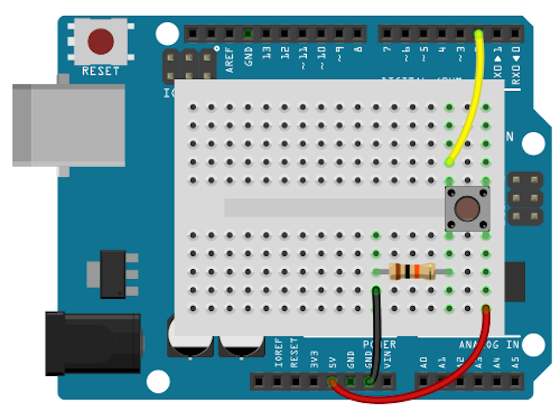
\includegraphics[height=0.4\textheight]{Kapitel1/Bilder/digitalreadserial2}}\qquad
\subfigure[Autoampel mit PushButton \label{fig:ampelButton}]{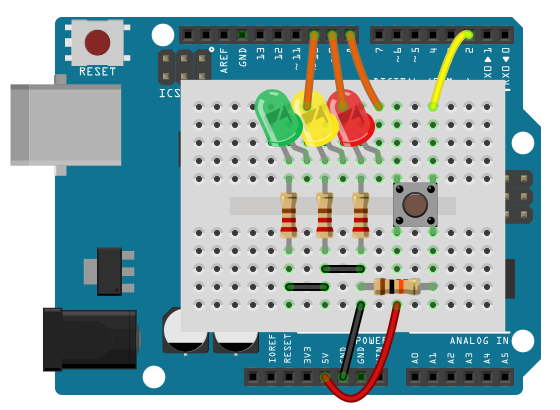
\includegraphics[height=0.4\textheight]{Kapitel1/Bilder/ampelButton}}
\caption{Das Schaltbild zum Beispiel Sketch ``DigitalReadSerial''}
\label{fig:digitalreadserial_schaltung}
\end{center}
\end{figure}



\subsection{Aufgaben}

\marginimage{Kapitel1/Bilder/10kOhm-button}

Erweitere deine Schaltung entsprechend Abb. \ref{fig:ampelButton}. Aus Platzgründen ist der PushButton näher an die rote LED eingebaut. Rechts wird der Platz noch gebraucht!
 
\subsubsection*{Aufgabe 1}

Testet die Schaltung zunächst mit dem Sketch ``DigitalReadSerial'' (siehe Listing \ref{lst:digitalreadserial}). Öffne den  ``Serieller Monitor'' im Menu ``Werkzeuge'' der Arduino LED. Schau dir die Ausgabe im ``Serieller Monitor'' an.

\subsubsection*{Aufgabe 2:}

Lies die Dokumentation zum DigitalReadSerial auf der Seite \ArduinoHomepage{en/Tutorial/DigitalReadSerial} genau durch und dokumentiere die folgenden Befehlen
  \begin{enumerate}
    \item Serial.begin()  (\ArduinoHomepage{en/Reference/Serial/Begin})
    \item Serial.println()  (\ArduinoHomepage{en/Reference/Serial/Println})
  \end{enumerate}
  
\subsubsection*{Aufgabe 3:}

Öffne dann den Sketch ``Button''  aus Beispiel/Digital. Schau die den Sketch genau an. Ergänze die Befehle (die noch nicht in deiner Tabelle dokumentiert sind) in deiner Tabelle. Schreibe den Sketch so um, dass die grüne LED verwendet wird.
\marginfigure{Kapitel1/Bilder/ampelFertig}{Push-Buttom mit LED}{fig:ampelButton}

\subsubsection*{Aufgabe 4: Projekt}

Erweitere deine Schaltung aus Aufgabe 3 entsprechend Abb. \ref{fig:ampelButton}, so dass du eine Autoampel (rot, gelb und grün) mit Fußgängerampel (rot und grün) mit Push-Button aufgebaut hast. Wenn ein Fußgänger auf den Kopf drückt (gedrückt hält), soll die Autoampel von grün auf rot schalten und die Fußgängerampel grün werden. Nach einer gewissen Zeit, soll die Autoampel wieder auf grün schalten.

\margininfo{Der Button muss lange gedrückt werden, da der Sketch nur an einer Stelle den Wert des Buttons auslesen kann. Später lernst du, wie du den Arduino programmieren kannst, damit er zu jeder Zeit den Button auslesen kann.}

\begin{multicols}{2}
\null\vfill 
\begin{arduinoCode}{Fußgängerampel mit Push-Button}{lst:fussgaengerample}
         (*@ \tikzmark{if} @*)
 if (digitalRead(2)) {
    // Fussgaengerample soll von rot auf gruen schalten und nach vier Sekunden wieder auf rot
      
 }
 
\end{arduinoCode}
\vfill\null 
\columnbreak

\null\vfill
\begin{itemize}
  \itemsep15pt
  \item[] \tikzmarkcomment{item1}{Hier reagiert der Arduino auf das drücken des Push-Buttons}
\end{itemize}
\vfill \null

\begin{tikzpicture}[remember picture,overlay]
  \path[red, thick,-] (if.east) edge [out=+25 , in=180] (item1);
  
\end{tikzpicture}


\end{multicols}


\sectionInformatik{C Sprachelemente: Variablen}

Daten zu speichern und zu verarbeiten ist eine zentrale Aufgabe eines Mikrocontrollers oder Computers. Die Programmiersprache stellt für diesen Zweck extra Variablen bereit.   

Eine Variable kannst du dir wie eine Art Box vorstellen. In so einer Box kannst du Zahlen, Wörter oder andere Dinge ablegen und du kannst sie später wieder hervorholen, um mit ihnen zu arbeiten.  Zum Beispiel können Messdaten eines Sensors gespeichert oder/und der gespeicherte Wert für eine Berechnung oder Ausgabe ausgelesen und/oder übergeben werden.

In diesem Abschnitt lernst du, wie Variablen für unterschiedliche Aufgaben erzeugt und manipuliert werden können.

\subsection{Das Erzeugen von Variablen}

Bevor eine Variable im Sketch verwendet werden kann, muss die Variable deklariert werden, d.h. es muss eine Box erstellt werden. \margininfo{Das Erstellen einer Variablen wird deklarieren genannt.} Deklarieren einer Variablen bedeutet, dass im Mikrocontroller Speicherplatz für die Variable zur Verfügung gestellt wird. In diesem Speicherbereich wird der Typ, und gegebenenfalls schon ein Wert gespeichert. \margininfo{Das Zuweisen eines Wertes wird initialisieren  genannt.} Variablen müssen nicht gleich initialisiert (ein Wert zugewiesen) werden, wenn sie deklariert werden, aber es ist oft nützlich ihnen einen definierten Anfangswert zuzuweisen.

\begin{multicols}{2}
\null\vfill 
\begin{arduinoCode}{Deklaration und Initialisation}{lst:deklarationinitialisation}
 int inVar1; (*@ \tikzmark{dek} @*)
 inVar1 = 9; (*@ \tikzmark{ini} @*)
  
 int inVar2 = 0; (*@ \tikzmark{dek-ini} @*)
\end{arduinoCode}
\vfill\null 
\columnbreak

\null\vfill
\begin{itemize}
  \itemsep15pt
  \item[] \tikzmarkcomment{item1}{Deklaration einer Variablen \textbf{inVar1}}
  \item[] \tikzmarkcomment{item2}{Initialisation einer Variablen \textbf{inVar1}}

  \item[] \tikzmarkcomment{item3}{Deklaration und Initialisation der Variablen \textbf{inVar2}}
\end{itemize}
\vfill \null

\begin{tikzpicture}[remember picture,overlay]
  \path[red, thick,-] (dek.east) edge [out=0 , in=180] (item1);
  \path[red, thick,-] (ini.east) edge [out=0 , in=180] (item2);
  \path[red, thick,-] (dek-ini.east) edge [out=0 , in=180] (item3);
\end{tikzpicture}


\end{multicols}

\subsection{Sinnvolle Namensgebung für Variablen}

Es ist extrem wichtig sinnvolle Namen für Variablen zu vergeben, damit sind Namen gemeint, die sich nach Möglichkeit selbst erklären. Doener1, doener2 mag zwar sehr lustig sein, aber du hast in zwei Wochen keine Ahnung mehr was du damit speichern wolltest! Darüber hinaus stellen die Variablen Doener und doener zwei Unterschiedliche Boxen dar. C unterscheidet Groß- und Kleinschreibung! \margininfo{C ist case sensitiv, das bedeutet die Variablennamen name, Name, NAME und naMe bezeichnen verschiedene Variablen}

\subsubsection{Tipps für sinnvolle Namen von  Variablen:}
Wenn du folgende Tipps befolgst, dann wirst du weniger Probleme haben!
\begin{itemize}
  \item Benenne deine Variable nach dem Inhalt: Wenn der Messwert eines Temperatur-Senors gespeichert werden soll ist ein sinnvoller Name measTemp (eng. measure messen).
  \item Benutzte die camelCase-Notation, d.h. der erste Buchstabe eines Variablennamens wird immer klein geschrieben. Wenn die Variable aus mehreren Wörtern zusammengesetzt ist, wird jedes Wort mit einem großen Buchstaben angefangen. Bekanntes Beispiel dieser Notation sind die Namen von Apple-Produkten:  iPhone, iPad, iPod, iMac aber auch McDonalds.
  \item Es gibt verschieden Variable-Typen. Oft ist es sinnvoll dass der Type der Variablen im Namen ablesbar ist. Zum Beispiel eine Variable die nur ganze Zahlen enthält wäre intVar eine gute Wahl. 
  \item Verwende nie ä,ö,ü oder ß. Diese Buchstaben werden vom C und der ArduinoIDE nicht unterstützt. Sonderzeichen (!, ?, /, - \_, \# etc.)  gehen auch nicht, diese Zeichen sind für (Rechen-) Operationen in C reserviert.    
\end{itemize}
Du wirst viele Beispiel-Sketche kennenlernen, die nicht der camelCase-Notation folgen. Das muss man auch nicht! Es macht aber Sinn, bestimmte sinnvolle Regeln bei der Vergabe von Namen in Programmen und für Dateinamen zu befolgen. Da sonst (bei größeren Programmen und vielen Dateien) sehr viel Zeit für die Suche nach Fehlern oder der richtigen Datei verloren geht!  Deshalb ist es sinnvoll, die camelCase-Notation von Anfang an immer zu benutzen.

\marginimage{Kapitel1/Tikz/camelCase}    

\subsection{Boxen mit Inhalt füllen}

Wenn eine Variable deklariert ist, kann ihr während des Programmablaufes mit Hilfe des Zuweisungsoperators 
(``='' Einfaches Gleichheitszeichen) ein Wert zugewiesen werden. Das Gleichheitszeichen ``='' hat die Aufgabe den Inhalt rechts, in die links stehend Box zu legen. Das Gleichheitszeichen hat in C eine andere Bedeutung als in der Mathematik! Besser wäre die Verwendung eines Pfeils ``$<-$'', leider hat man sich für das ``='' Zeichen entschieden.    
\margininfo{Das Gleichheitszeichen ist in C ein Zuweisungsoperator!}
\clearpage

\begin{multicols}{2}
\null\vfill 
\begin{arduinoCode}{Verwenden von Variablen}{lst:verwendung}
 intVar = 7;  (*@ \tikzmark{setzen1} @*) 
 
 inputVariable2 = analogRead(A2); (*@ \tikzmark{setzen2} @*) 
\end{arduinoCode}
\vfill\null 
\columnbreak

\null\vfill
\begin{itemize}
  \itemsep25pt
  \item[] \tikzmarkcomment{item1}{Weist der Variablen intVar den Wert 7 zu.}
  \item[] \tikzmarkcomment{item2}{Weist der Variablen intVar2 den Wert des analogen PIN A2 zu.} 
\end{itemize}
\vfill \null

\begin{tikzpicture}[remember picture,overlay]
  \path[red, thick,-] (setzen1.east) edge [out=0 , in=180] (item1);
  \path[red, thick,-] (setzen2.east) edge [out=0 , in=180] (item2);
\end{tikzpicture}

\end{multicols}


Sobald eine Variable gesetzt wurde (ein Wert zugewiesen), kann mit ihrem Wert gearbeitet 
werden. Z.B. kann überprüft werden, dass bestimmte Bedingungen erfüllt sind, oder der Wert
kann auch direkt  verwendet werden. 

\subsection{Für jeden Inhalt die passende Box}

\begin{table}[h]

\begin{center}
\tikzset{ 
    table/.style={
        matrix of nodes,
        row sep=-\pgflinewidth,
        column sep=-\pgflinewidth,
        nodes={
            rectangle,
            draw=black,
            align=center
        },
        minimum height=1.5em,
        text depth=0.5ex,
        text height=2ex,
        nodes in empty cells,
%%
        every even row/.style={
            nodes={fill=gray!20}
        },
        column 1/.style={
            nodes={text width=0.15\textwidth}
        },
        column 2/.style={
            nodes={text width=0.2\textwidth}
        },
        column 3/.style={
            nodes={text width=0.65\textwidth}
        },
        row 1/.style={
            nodes={
                fill=black!80,
                text=white,
                font=\bfseries
            }
        }
    }
}

\begin{tikzpicture}
\matrix (first) [table,text width=6em]
{   
  Variablentyp & Bedeutung  & Beschreibung \\
  int & Integer & ganze Zahlen (-32.768 bis 32.767) \\
  long & ganze Zahlen & (-2 Milliarden bis 2 Milliarden)\\
  float & Fließkommazahl & gebrochene Zahlen \\
  char & Character & Alphanumerische Zeichen (Buchstaben, Zahlen, Sonderzeichen) \\
  array & Variablenfeld & mehrere Werte eines Variablentyps können gespeichert werden \\
  String & Zeichenkette & Array aus mehreren alphanumerischen Zeichen \\
};
 \end{tikzpicture}
\end{center}
\caption{Auswahl an verschiedenen Variablentypen}
\label{tab:varTyps}
\end{table}%

Die beiden Variablentypen array und String sind etwas komplizierter aufgebaut und werden deshalb hier noch näher besprochen: 

\subsubsection{Arrays}

Bei Arrays handelt es sich im Grunde nicht um einen eigenen Typ von Variablen, sondern um eine Gruppierung mehrerer Variablen eines Typs.
\begin{arduinoCode}{}{}
int meineWerte[5] = {10,12,32,46,50};
\end{arduinoCode}
Im Beispiel wird als erstes ein Array vom Typ int angelegt. Die 5 in eckigen Klammern hinter dem Namen der Variable bestimmt die Anzahl der Speicherplätze, die das Array bereit stellt. Man nennt die Anzahl der Speicherplätze auch die Länge des Arrays.

Im Programm kann man durch die Verwendung eines Index auf die Speicherplätze des Arrays zugreifen. Die erste Stelle im Array ist die Stelle 0: meineWerte[0], der Wert ist 10 usw.

\begin{multicols}{2}
\null\vfill   
\begin{arduinoCode}{}{}
analogWrite(ledPin, meineWerte[0]); (*@ \tikzmark{mW0} @*)
analogWrite(ledPin, meineWerte[1]); (*@ \tikzmark{mW1} @*)
...
analogWrite(ledPin, meineWerte[4]); (*@ \tikzmark{mW4} @*)
\end{arduinoCode}
\vfill\null 
\columnbreak

\null\vfill
\begin{itemize}
  \itemsep15pt
  \item[] \tikzmarkcomment{item1}{Erster Wert: 10}
  \item[] \tikzmarkcomment{item2}{Zweiter Wert: 12}
    \item[] \tikzmarkcomment{item3}{Letzter Wert: 50}
\end{itemize}
\vfill \null

\begin{tikzpicture}[remember picture,overlay]
  \path[red, thick,-] (mW0.east) edge [out=0 , in=180] (item1);
  \path[red, thick,-] (mW1.east) edge [out=0 , in=180] (item2);
  \path[red, thick,-] (mW4.east) edge [out=0 , in=180] (item3);
\end{tikzpicture}


\end{multicols}


\subsubsection{String}
Es gibt verschiedene Möglichkeiten Textstrings darzustellen. Man kann entweder den Datentyp String verwenden oder einen String aus einem Array von Daten des Types char erstellen.
 
\begin{arduinoCode}{}{}
  String str1 = "arduino";
  char str2[8] = {'a', 'r', 'd', 'u', 'i', 'n', 'o'};
  char str3[ ] = "arduino";
  char Str4[8] = "arduino";
\end{arduinoCode}
Alle erzeugten Textstrings haben denselben Inhalt.


\subsubsection{Aufgabe 1}
Es gibt weitere Variablen-Typen. Informiere dich auf der Arduino Homepage \ArduinoHomepage{en/Reference/HomePage} über folgende Typen: 
boolean, unsigned int, short, double. 
Notiere ihre Bedeutung, ihre Beschreibung analog zur Tabelle \ref{tab:varTyps}.

\subsubsection{Aufgabe 2 (Projekt)}
Wie dir vielleicht aufgefallen ist, steht auf der Arduino Homepage \ArduinoHomepage{en/Reference/HomePage}  zweimal der Begriff String. Einmal klein und einmal groß geschrieben (siehe Abb. \ref{fig:string}). Das ist kein Fehler, sondern es sind wirklich zwei unterschiedliche Dinge. 

\begin{itemize}
  \item[] \textbf{string} bezeichnet ein Array, bei dem in jedem Feld Daten des Typs char gespeichert sind. 
  \item[] \textbf{String}: wiederum ist ein Text-Objekt. Objekt bedeutet in diesem Zusammenhang, dass es spezielle Funktionen gibt, mit welchen die im Objekt gespeicherten Daten manipuliert werden können. Funktionen die zu einem Objekt gehören, werden Methoden genannt.
\end{itemize}

\marginfigure{Kapitel1/Bilder/String.png}{Aufzug Arduino Homepage}{fig:string}

Objekte sind in der Informatik extrem wichtig. Mit dieser Aufgabe hast du die Möglichkeit einen ersten Blick auf sie zu werfen.

Auf der Seite \ArduinoHomepage{en/Reference/StringObject} werden die speziellen Funktionen anhand von Beispielen erklärt. Arbeite die zwei Punkte durch. Lade dazu den jeweiligen Beispiel-Sketch auf deinen Arduino und versuche zu verstehen was passiert. Beschreibe schriftlich in kurzen Sätzen deine Beobachtungen.
\begin{itemize}
  \item \ArduinoHomepage{en/Tutorial/StringConstructors}
  \item \ArduinoHomepage{en/Tutorial/StringAdditionOperator}
\end{itemize}


\subsection{Geltungsbereich von Variablen}

Für eine Variable wird immer (ihrem Typ entsprechend) eine bestimmte Größe an Speicherplatz reserviert. Die Größe dieses Speicherplatzes bestimmt den Wertebereich der Variablen.

%In Abb. \ref{fig:geltungsbereich} ist der Geltungsbereich einer Variablen mit 3 Bit Speicherplatz als Zahlenkreis dargestellt. Mit 3 Bit können die Binärzahlen $000$, $001$, $010$, $011$, $100$, $101$, $110$ und $111$ dargestellt werden.  Diese Binärzahlen stellen die Dezimalzahlen von 0 bis 7 dar. Wird jetzt eine Bereichsüberschreitung, z.B. durch eine Addition verursacht, wird entsprechend im Zahlenkreis weitergegangen.  
%\margintikzfig{\begin{tikzpicture}
%\def \n {7}
%\def \radius {2cm}
%\def \margin {8} % margin in angles, depends on the radius
%
%\foreach \s in {0,...,\n}
%{
%  \node[draw, circle] at ({360/(\n+1) * (\s)}:\radius) {$\s$};
%  \draw[->, >=latex] ({360/(\n+1) * (\s)+\margin}:\radius) 
%    arc ({360/(\n+1) * (\s)+\margin}:{360/(\n+1) * (\s+1)-\margin}:\radius);
%}
%\end{tikzpicture}
%}{Geltungsbereich einer 3 Bit Variablen}{fig:geltungsbereich}


Bei einer integer Variable ist der Wertebereich alle ganzen Zahlen zwischen $-32768$ und $32767$. Wenn man nun versucht einen größeren Wert z.B. 32770 in einer integer Variablen zu speichern wird eine sogenannte Wertebereich-Überschreitung (oder Überlauf) erfolgen. Beim Arduino wird um den zu großen Wert zu speichern einfach zum negativen Bereich ``weitergegangen''. Das heißt es wird der Wert $-32765$ gespeichert.
\begin{multicols}{2}
\null\vfill    
\begin{arduinoCode}{Überlauf einer integer Variablen}{lst:geltungsbereich}
  gBer = -32768; 
  gBer = gBer - 1;  (*@ \tikzmark{neg} @*)
  
  gBer = 32767;
  gBer = gBer + 1;  (*@ \tikzmark{pos} @*)
  
\end{arduinoCode}
\vfill\null 
\columnbreak

\null\vfill
\begin{itemize}
  \itemsep15pt
  \item[] \tikzmarkcomment{item1}{Wert der Variable ist jetzt 32767}
  \item[] \tikzmarkcomment{item2}{Wert der Variable ist jetzt -32768}
\end{itemize}
\vfill \null

\begin{tikzpicture}[remember picture,overlay]
  \path[red, thick,-] (neg.east) edge [out=0 , in=180] (item1);
  \path[red, thick,-] (pos.east) edge [out=0 , in=180] (item2);
\end{tikzpicture}
\end{multicols}

\subsubsection{Aufgabe 3}
Verändere \textbf{nichts} an deiner Schaltung. Erstelle den Sketch ``Ueberlauf''. Die Aufgabe ist, den Überlauf  der integer Variablen \textbf{gBer} ververanschaulichen. Führe dazu die Operationen aus Listing \ref{lst:geltungsbereich} in die setup()-Methode ein und übermittle mit Hilfe des Befehls Serial.println(gBer) den aktuellen Wert der Variablen gBer.  

\begin{multicols}{2}  
\begin{arduinoCode}{Versuche zur Überlauf einer Variablen}{lst:versuch-geltungsbereich}
int gBer; 
  
void setup() {
  Serial.begin(9600);
          (*@ \tikzmark{op} @*)
  Serial.println(gBer); (*@ \tikzmark{ser} @*)
}

void loop() {  
}
\end{arduinoCode}
\vfill\null 
\columnbreak

\null\vfill
\begin{itemize}
  \itemsep15pt
  \item[] \tikzmarkcomment{item2}{Füge die einzelnen Operationen aus Listing \ref{lst:geltungsbereich} ein}
  \item[] \tikzmarkcomment{item3}{Gibt nach jeder Operation den aktuellen Wert der Variablen aus}
  

\end{itemize}
\vfill \null

\begin{tikzpicture}[remember picture,overlay]
  \path[red, thick,-] (op.east) edge [out=0 , in=180] (item2);
  \path[red, thick,-] (ser.east) edge [out=0 , in=180] (item3);
\end{tikzpicture}
\end{multicols}

Lade deinen fertigen Sketch auf das Arduino-Board und öffne die Serielle Verbindung zum Arduino-Board. Dokumentiere deine Ergebnisse.




% Kapitel 2 %
\chapter{Sensoren}

\epigraph{We can only see a short distance ahead, but we can see plenty there that needs to be done.}{Alan Turing (1912-1954) britischer Logiker, Mathematiker und Kryptoanalytiker}

\subsubsection{Was du in diesem Kapitel lernen wirst}
\begin{itemize}
  \item Funktionsweise von analogen und digitalen Sensoren
  \item Verwendung von Unterprogrammen und Kontrollstrukturen in C
  \item Funktionsweise eines Spannungteilers 
  \item Messen von Temperatur, Entfernung, Licht und Farben, Luftfeuchte
  \item Verwendung eines Multimeters 
  \item Das Verwenden von Objekten und Methoden 
\end{itemize}


% Kapitel 2 %

\section{Analoger Sensor: Der Temperatur-Sensor LM35 und LM36}
\label{sec:lm35}
Die Temperatursensoren LM35 und LM36 oder die Funktionsgleichen TMP35 TMP36 sind sogenannte analoge Sensoren. Analoge Sensoren haben meistens 3 PINs. Zwei PINs werden zur Spannungsversorgung (U$_S$ und GND) und einer PIN (V$_{out}$) für den Messwert benötigt. Dabei variiert die Spannung an V$_{out}$ linear mit 10mV pro $1^\circ$C\footnote{Eigentlich werden Temperaturunterschiede in Grad Kelvin K angegeben.}. Beim LM35 entspricht einer Spannung von 0mV dem Temperaturwert von $0^\circ$C. Da mit dem TMP36 auch negative Temperaturen gemessen werden können entspricht eine Spannung von 0mV ca. dem Temperaturwert -$50^\circ$C (siehe Abb. \ref{fig:daten-tmp36}). 
\begin{figure}[h]
  \begin{center}
  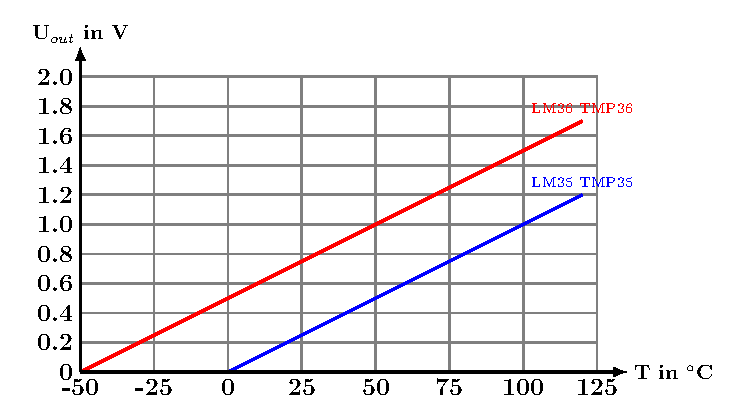
\includegraphics[width=0.55\textwidth]{Kapitel2/Tikz/lm35temp.pdf}
  \caption{Temperatur Ausgangsspannungs Verlauf des LM35}
  \label{fig:daten-tmp36}
  \end{center}
\end{figure}

\marginfigure{Kapitel2/Bilder/lm35}{PIN Belegung}{fig:lm35}

Solche Informationen erhält man aus einem sogenannten Datenblatt. Jeder Hersteller liefert ein mehr oder weniger ausführliches Datenblatt, das den Aufbau und die Funktion des Bauteils beschreibt. 
Für die Temperatursensoren kann anhand dieser Informationen eine Formel zur Berechnung des Temperaturwerts hergeleitet werden. Für den LM35 und TMP35 ergibt sich die Formel (\ref{eqn:lm35}) und für den LM36 und TMP36 die Formel (\ref{eqn:tmp36}):
\begin{multicols}{2}
\begin{equation}\label{eqn:lm35}
 T(V_{out}) = \frac{V_{out}}{10}
\end{equation}
\begin{equation}\label{eqn:tmp36}
 T(V_{out}) = \frac{V_{out} - 500}{10}
\end{equation}
\end{multicols}

\subsection{Der Beipiel-Sketch} 

Wenn zur Messung der Temperatur eine Verarbeitung der gemessenen Werte am analogen Eingang nötig sind, ist es für die Übersicht des Sketches sinnvoll, diese Berechnung in einer sog. Funktion auszulagern. Der Vorteil ist, dass wenn man den Sensor gegen einen anderen Sensor austauscht, bei dem die Messgröße anhand einer anderen Formel berechnet werden muss, dann findet die Anpassung nur in dieser Funktion statt.     

\begin{multicols}{2}
\begin{arduinoCode}{Testsketch ``TempTest'' für einen Temperatursensor LM35}{lst:temp}
int senPin = A0; (*@ \tikzmark{senPin} @*)
int VS = 5000;(*@ \tikzmark{vs} @*)
float temp = 0.0; 
 
void setup() {
  Serial.begin(9600);
}
 
void loop() {
  temp =  getTemperature(); (*@ \tikzmark{fktauf} @*)
  Serial.print( temp );
  Serial.println(" C");
}
 
float getTemperature() { 
  int senV = analogRead(senPin); 
  float t = map(senV,0,1023,0,VS)/10.0;(*@\tikzmark{funk_def} @*)
  return t;
}
\end{arduinoCode}

\vfill\null 
\columnbreak

\null\vfill
\begin{itemize}
  \itemsep15pt
    \item[] \tikzmarkcomment{item1}{Definition des Sensor PINs}
    \item[] \tikzmarkcomment{item2}{Versorgungsspannung in mV}
    \itemsep35pt
    \item[] \tikzmarkcomment{item3}{Die Funktion wird aufgerufen}
    \itemsep45pt
    \item[] \tikzmarkcomment{item4}{Definition der Funktion für  einen LM36 muss diese Zeile abgeändert werden: \\ \small{\textbf{float temp = (map(senV,0,1023,0,VS)-500)/10;}}}
\end{itemize}
\vfill \null

\begin{tikzpicture}[remember picture,overlay]
  \path[red, thick,-] (senPin.east) edge [out=0 , in=180] (item1);
  \path[red, thick,-] (vs.east) edge [out=0 , in=180] (item2);
  \path[red, thick,-] (fktauf.east) edge [out=0 , in=180] (item3);
  \path[red, thick,-] (funk_def.east) edge [out=0 , in=180] (item4);
\end{tikzpicture}


\end{multicols}

\marginfigure{Kapitel2/Bilder/temperatursensor}{Temperatursensor LM35CZ}{fig:temp}
\subsection{Aufgaben}

Baue die abgebildete Schaltung (Abb. \ref{fig:temp}) auf. Achte auf die Beschriftung und somit auf den richtigen Einbau des Temperatur-Sensors. Sollte sich der Temperatursensor, nachdem du den Arduino mit dem PC verbunden hast sehr schnell erwärmen, dann hast du den Sensor falsch eingebaut! Unterbreche die Verbindung zum PC und überprüfe den richtigen Einbau. Wenn der Temperatursenor sich zu sehr erwärmt, kann er zerstört werden! 
 
\subsubsection{Aufgabe 1}
Erstelle und lade den Beispiel-Sketch ``TempTest'' \ref{lst:temp} auf deinen Arduino und öffne dann die serielle Verbindung. Messe verschiedene Temperaturen.


\subsubsection{Aufgabe 2}
\margininfo{if ist eine bedingte Anweisung (siehe Kapitel \ref{sec:bedingte-Anweisung})}

Baue mit Hilfe des Temperatursensor und den drei LEDs (grün, gelb und rot) ein Thermometer bei dem bis zur 
Temperatur 20$^{\circ}$C nur die grüne LED leuchtet, bis 25$^{\circ}$C die grüne und gelbe LED leuchten und ab 30$^{\circ}$C die grüne, gelbe und rote LED leuchten. 
Füge dazu den Code in die loop()-Routine ein und ergänze entsprechend. In Kapitel \ref{sec:bedingte-Anweisung} erfährst du mehr über bedingte Anweisugen. 

\begin{arduinoCode}{}{}
if (temp > 20) {
  // gruen an, gelb rot aus
}
if (temp > 25) {
  // gruen gelb an, rot aus
}
if (temp > 30) {
  // gruen gelb rot an
}
\end{arduinoCode}


\subsubsection{Aufgabe 3 (Projekt)}%

In Amerika werden normalerweise Temperaturen in Fahrenheit $F$ angegeben. Die Umrechnung ist einfach: 
\begin{equation}
 F(T) = T\cdot 1.8 + 32
\end{equation}
Schreibe eine weiter Funktion getFahrenheit(), die die gemessene Temperatur in Fahrenheit berechnet. Übermittle mit Hilfe einer seriellen Verbindung den gemessenen Temperaturwert in Grad Celsius und Fahrenheit an den PC.

Die wichtigste Temperaturskala ist die Kelvin-Skala. Bei der Kelvin Skale entspricht die Temperatur am absoluten Nullpunkt 0K und bei $0^{\circ}$C umgerechnet 273,15K. 

Es gibt noch weitere Temperaturskalen. Suche in Wikipedia nach dem Schlagwort ``Temperaturskala''. Entwerfe weiter Unterprogramme für die Temperaturskalen: Kelvin und Rømer

\begin{multicols}{2}
\begin{arduinoCode}{}{}
float GetFahrenheit(int vs) { 
  int senV = analogRead(senPin); 
  float temp = (map(senV,0,1023,0,vs)-500)/10;
         (*@ \tikzmark{umrechnung} @*)   
  return fahrenheit;
\end{arduinoCode}
\vfill\null 
\columnbreak

\null\vfill
\begin{itemize}
  \itemsep15pt
    \item[] \tikzmarkcomment{item1}{Umrechnung von Grad Celsius nach Fahrenheit}
 \end{itemize}
\vfill \null

\begin{tikzpicture}[remember picture,overlay]
  \path[red, thick,-] (umrechnung.east) edge [out=0 , in=180] (item1);
\end{tikzpicture}
\end{multicols}

 
  
 
\sectionInformatik{C Sprachelemente: Unterprogramme}
Der Einsatz eines Unterprogramm ist sinnvoll, um das Programm übersichtlich zu halten. Wenn z.B. das Auslesen und Berechnen einer Messgröße eines Sensors aufwendig ist, wird der Sketch übersichtlicher, wenn dieser Teil des Programms aus der loop()-Routine in ein eigenes Unterprogramm ausgelagert wird. Unterprogramme werden dann unverzichtbar, wenn einzelne Programmteile sich wiederholen. Wenn diese Teile nicht in ein Unterprogramm ausgelagert werden und später Änderungen vorgenommen werden, dann müssen diese Änderungen an verschiedenen Stellen vorgenommen werden. Wenn ein Unterprogramm benutzt wird, muss nur an einer einzigen Stelle etwas verändert werden!

\margininfo{Don’t repeat yourself -- DRY}

\subsection{Allgemeiner Aufbau eines Unterprogrammes in C}

Ein Unterprogramm besteht aus zwei Teilen: einem Kopf und einen Körper. Im Kopf wird der Typ, der Name und eventuelle Eingabeparameter festgelegt. Der Körper besteht aus den eigentlichen Anweisungen und einem eventuellen Rückgabewert.
\begin{multicols}{2}
\null\vfill
\begin{arduinoCode}{Aufbau eines Unterprogrammes}{lst:c-function}
  (*@ \tikzmark{fktTyp} @*)        (*@ \tikzmark{fktParameter} @*)
type Name(parameter){
       (*@ \tikzmark{fktName} @*)
    
  (*@ \tikzmark{fktBody} @*)  


  return rueckgabeWert; (*@ \tikzmark{fktReturn} @*)
}           
\end{arduinoCode}
\vfill\null 
\columnbreak
\vfill\null 
\begin{itemize}
  \itemsep15pt
    \item[] \tikzmarkcomment{item1}{Unterprogramm Type: z.B. int oder boolean}
    \item[] \tikzmarkcomment{item2}{Parameter: ein Wert, der übergeben wird}
    \item[] \tikzmarkcomment{item3}{Name des Unterprogramm}
    \item[] \tikzmarkcomment{item4}{Unterprogramm Code}
    \item[] \tikzmarkcomment{item5}{Rückgabewert: Wert der zurückgegeben wird}
 \end{itemize}
\vfill \null

\begin{tikzpicture}[remember picture,overlay]
  \path[red, thick,-] (fktTyp.east) edge [out=25 , in=180] (item1);
  \path[red, thick,-] (fktParameter.east) edge [out=25 , in=180] (item2);
  \path[red, thick,-] (fktName.east) edge [out=-15 , in=180] (item3);
  \path[red, thick,-] (fktBody.east) edge [out=0 , in=180] (item4);
  \path[red, thick,-] (fktReturn.east) edge [out=0 , in=180] (item5);
\end{tikzpicture}
\end{multicols}


Unterprogramme können anhand ihres Types unterschieden werden. So kann man Unterprogramme ohne Rückgabewert Prozeduren und Unterprogramme mit Rückgabewert Funktionen nennen.
\margininfo{In vielen Programmiersprachen werden die Begriffe Unterprogramm und Funktion synonym verwendet.}

\subsection{Unterprogramm ohne Rückgabewert -- Prozeduren}
Unterprogramme die keinen Rückgabewert haben, werden Prozeduren genannt. Du solltest zwei Prozeduren schon gut kennen: Die setup()- und loop()-Prozeduren. Das Type-Schlüsselwort ist void (eng. für leer). 

\subsubsection{Beispiel: Die Reset()-Prozedur}
Manchmal ist es sinnvoll den Arduino Softwaretechnisch neu zu starten. Eine einfache Lösung stellt die Verwendung des Reset-PINs dar. Wenn am Reset-PIN HIGH anliegt wird der Arduino neue gestartet. Dies kann zum Beispiel mit einem Push-Buttom realisiert werden, oder mit Hilfe eines digitalen PINs.

\marginfigure{Kapitel2/Bilder/reset.png}{Reset Prozedure}{fig:reset}

\begin{multicols}{2}
\null\vfill
\begin{arduinoCode}{Reset()-Prozedur}{lst:reset}
  (*@ \tikzmark{fktTyp} @*)
void Reset() (*@ \tikzmark{fktName} @*)
{      
  int resetPin=12;
  pinMode(resetPin, OUTPUT);     (*@ \tikzmark{fktBody} @*)  
  digitalWrite(resetPin, HIGH);    
}
\end{arduinoCode}

\vfill\null 
\columnbreak
\vfill\null 
\begin{itemize}
  \itemsep20pt
    \item[] \tikzmarkcomment{item1}{\textbf{void} bedeutet, dass die Prozedur keine Rückgabewert hat}
    \item[] \tikzmarkcomment{item2}{Name des Unterprogramm}
    \item[] \tikzmarkcomment{item3}{Der Arduino wird mit Hilfe des Reset-PINs und PIN 12 neu gestartet}
 \end{itemize}
\vfill \null

\begin{tikzpicture}[remember picture,overlay]
  \path[red, thick,-] (fktTyp.east) edge [out=25 , in=180] (item1);
  \path[red, thick,-] (fktName.east) edge [out=0 , in=180] (item2);
  \path[red, thick,-] (fktBody.east) edge [out=0 , in=180] (item3);
\end{tikzpicture}
\end{multicols}

Es gibt Lösungen ohne die Verwendung des Reset-PINs. Wenn man mit den Schlagwörtern Watchdog und Reset Function sucht, findet man schnell solche Lösungen. Aber es ist Vorsicht geboten, wenn eine solche Reset-Prozedure zu schnell aufgerufen wird, startet der Arduino neue bevor der Bootloader einen neuen Sketch aufspielen kann. Damit wird der IC unbrauchbar und muss ausgetauscht werden.    

\pagebreak
\subsection{Unterprogramm mit Rückgabewert -- Funktion}
Unterprogramme werden als Funktion bezeichnet, wenn sie einen Wert zurückliefen.

\subsubsection{Beispiel: }

Oft wird die Zeit benötigt, die ein Taster gedrückt wird. Es gibt zwar einen Arduino Befehl dafür (pulseIn()), aber durch die Verwendung einer Funktion wird der Sketch übersichtlicher.  

\begin{multicols}{2}
\null\vfill
\begin{arduinoCode}{ pushedTime()-Funktion }{lst:pushedTime}
  (*@ \tikzmark{fktTyp} @*)
int pushedTime()  (*@ \tikzmark{fktName} @*)
{       
  return pulseIn(pushPIN, HIGH); (*@ \tikzmark{fktReturn} @*)
  
}
\end{arduinoCode}

\vfill\null 
\columnbreak
\vfill\null 
\begin{itemize}
  \itemsep15pt
  \item[] \tikzmarkcomment{item1}{Der Rückgabewert ist vom Type \textbf{integer}}
  \item[] \tikzmarkcomment{item2}{Name des Unterprogramm}
  \item[] \tikzmarkcomment{item3}{Rückgabewert: Wert der zurückgegeben wird}
 \end{itemize}
\vfill \null

\begin{tikzpicture}[remember picture,overlay]
  \path[red, thick,-] (fktTyp.east) edge [out=25 , in=180] (item1);
  \path[red, thick,-] (fktName.east) edge [out=0 , in=180] (item2);
  \path[red, thick,-] (fktReturn.east) edge [out=0 , in=180] (item3);
\end{tikzpicture}
\end{multicols}


\subsection{Unterprogramm mit Parameter}

Parameter können an das Unterprogramm übermittelt werden,
so ist es möglich, dass Informationen von Hauptprogramm zum Unterprogramm übermittelt werden.  

\clearpage
\begin{multicols}{2}
\null\vfill
\begin{arduinoCode}{ blinkLED()-Parameter }{lst:reset}
  (*@ \tikzmark{fktTyp} @*)     (*@ \tikzmark{fktName} @*)         (*@ \tikzmark{fktParameter} @*)
void blinkLED(int ledPIN)
{
  pinMode(ledPIN, OUTPUT);    
  digitalWrite(ledPIN, HIGH);
  delay(1000);                  (*@ \tikzmark{fktBody} @*)
  digitalWrite(ledPIN, LOW);
  delay(1000);  
}
\end{arduinoCode}
\vfill\null 
\columnbreak
\vfill\null 
\begin{itemize}
  \itemsep15pt
    \item[] \tikzmarkcomment{item1}{\textbf{void} also keine Rückgabewert}
    \item[] \tikzmarkcomment{item2}{Name des Unterprogramm}
    \item[] \tikzmarkcomment{item3}{Parameter: digitaler PIN}
    \item[] \tikzmarkcomment{item4}{Eine LED am blinkt mit einer Sekunde}
 \end{itemize}
\vfill \null

\begin{tikzpicture}[remember picture,overlay]
  \path[red, thick,-] (fktTyp.east) edge [out=25 , in=180] (item1);
  \path[red, thick,-] (fktName.east) edge [out=15 , in=180] (item2);
  \path[red, thick,-] (fktParameter.east) edge [out= 5 , in=180] (item3);
  \path[red, thick,-] (fktBody.east) edge [out=0 , in=180] (item4);
\end{tikzpicture}
\end{multicols}

\subsection{Aufgaben:}

\subsubsection{Aufgabe 1:}

Du hast jetzt schon einige Arduino Befehle kennengelernt und in deiner Befehlsübersicht dokumentiert! Ordne die Befehle, die Unterprogramme sind in einer Tabelle. Unterscheide die Befehle nach Prozedur, Funktion und Unterprogramme mit Parameter. Einzelne Befehle können auch in mehrmals auftauchen. In Abb. \ref{tab:unterprogramme} ein.

\begin{figure}[h]
  \begin{center}
  \tikzset{ 
      table/.style={
          matrix of nodes,
          row sep=-\pgflinewidth,
          column sep=-\pgflinewidth,
          nodes={
              rectangle,
              draw=black,
              align=center
          },
          minimum height=1.5em,
          text depth=0.5ex,
          text height=2ex,
          nodes in empty cells,
  %%
          every even row/.style={
              nodes={fill=gray!20}
          },
          column 1/.style={
              nodes={text width=0.3\textwidth}
          },
          column 2/.style={
              nodes={text width=0.6\textwidth, align=left}
          },
          row 1/.style={
              nodes={
                  fill=black!80,
                  text=white,
                  align=center,
                  font=\bfseries
              }
          }
      }
  }
  \begin{tikzpicture}
  \matrix (first) [table,text width=6em]
  {   
   Unterprogramm Typ:   & Arduino Befehle \\
   Prozeduren       &  setup() \\
   Funktion         &  digitalRead(PIN) \\
   Unterprogramm mit Parameter &  delay(1000) \\
  };
  \end{tikzpicture}
  \caption{Arduino Befehle sind Unterprogramme}
  \label{tab:unterprogramme}
  \end{center}
\end{figure}

\subsubsection{Aufgabe 2: Der SOS-Sketch mit Unterprogrammen} 

In Kapitel 1 hast du den Sketch ``SOS'' geschrieben, der mit Hilfe einer LED an PIN 10 den Morsecode SOS (kurz kurz kurz, lang lang lang, kurz kurz kurz) optisch sendet. Öffne diesen Sketch und analysiere ihn. Zwei Sachverhalte wirst du wahrscheinlich feststellen:

\begin{itemize}
\item[1.] Du wirst Schwierigkeiten haben deinen Sketch schnell zu verstehen! 
\item[2.] Wenn du die Zeiten für die lange Leuchtdauer verdoppeln möchtest, dann muss du das an sehr vielen Stellen machen. 
\end{itemize}

Der Sketch ist unübersichtlich, da sehr oft hintereinander sehr ähnlicher Code steht. Mit Hilfe der Prozeduren lang() und kurz() dann die loop()-Methode vereinfacht werden. Füge den Beispielcode aus Listing \ref{lst:lang_kurz} nach der loop()-Methode in den Sketch ein und vervollständige die Prozedur kurz(). Ersetzt in deiner loop()-Methode den jeweiligen Code durch den Aufruf der Prozedur kurz() oder lang() (siehe Listing \ref{lst:lang_kurz}). 

\begin{multicols}{2}
\null\vfill
 
\begin{arduinoCode}{ Die Prozeduren lang() und kurz() }{lst:lang_kurz}
void lang() {
  // led soll 2 Sekunden leuchten
  digtialWrite(10, HIGH);
  delay(2000);
  digtialWrite(10, LOW);
  delay(1000);
}

void kurz() {
  // led soll 1 Sekunden leuchten
}  
\end{arduinoCode}
\vfill\null 
\columnbreak
\vfill\null 
\begin{arduinoCode}{ Die Prozeduren blink(int time) }{lst:blink_mit_parameter}
void blink(int time) {
  digtialWrite(10, HIGH);
  delay(time);
  digtialWrite(10, LOW);
  delay(1000);
}
\end{arduinoCode}
\end{multicols}

Jetzt sollte deine loop()-Prozedur schon viel einfacher aussehen. Aber eigentlich machen deine beiden Prozeduren, mehr oder wenige das selbe. Erstelle jetzt eine Prozedur blink() mit dem Parameter time (siehe Listing \ref{lst:blink_mit_parameter}). Vereinfache deinen Sketch weiter und dokumentier ihn ausführlich.

\clearpage
\section{Widerstände und Spannungsteiler}
\label{sec:spannungsteiler}
Würde man einen digitalen Pin mit 5 Volt verbinden, so läge (wenn der digitale Pin auf INPUT gestellt ist) der Zustand ``HIGH'' an. Auf der anderen Seite, den nun GND mit dem digitalen Pin verbunden wäre, so läge der Zustand ``LOW'' an. Was wäre, wenn man den digitalen Pin sowohl mit 5Volt und mit GND verbindet? Ist der anliegende Zustand dann ``HIGH``oder ``LOW''? Leider würde es einen Kurzschluss geben, da 5 Volt direkt mit GND verbunden wäre, und kein Strombegrenzer (LED mit Vorwiderstand, Lautsprecher, Motor oder ähnliches) vorhanden ist, steigt der Strom soweit an, bis er über den maximal zulässige Strom von 500mA liegt. Der Spannungsregler wird überhitzen und sich hoffentlich rechtzeitig abschalten, bevor etwas kaputt geht. 

Interessanter wird es, wenn man die beiden Verbindungen vom digitalen Pin zu GND bzw. vom digitalen Pin zu 5V jeweils mit Widerständen verbindet. So entsteht kein Kurzschluss, da nur ein schwacher Strom durch die beiden Widerstände am Mikrocontroller vorbei fließt. Diese Schaltung bezeichnet man als Spannungsteiler (siehe Abb. \ref{fig:spannungsteiler}).

\margintikzfig{\begin{circuitikz} \draw
 (0,0) node[anchor=east]{GND}
  to[short, o-*] (1,0)
  to[generic, l=$R_{down}$, *-*] (1,2)
  (1,2) to[short, *-o] (0,2)
  node[anchor=east]{Pin02}
  (1,2) to[R, l=$R_{up}$] (1,4)
 (1,4) to[short, *-o] (0,4)
  node[anchor=east]{+5V}
;\end{circuitikz}}{Spannungsteiler}{fig:spannungsteiler}



Der Pull-Up-Widerstand $R_{up}$ und der Pull-Down-Widerstand $R_{down}$ teilen sich die 
Gesamtspannung entsprechend ihrer Anteile am Gesamtwiderstand in die Spannung 
$U_{up}$ und $U_{down}$ auf. Das Potential am digitalen Pin des Arduinos entspricht 
$U_{down}$ und lässt sich aus den Widerstandswerten und der Gesamtspannung $U_{ges}$ berechnen:



\begin{eqnarray}\label{eqn:spannungsteiler}
U_{down} = U_{ges} \cdot \frac{R_{down}}{R_{up} + R_{down}}
\end{eqnarray}

\subsection{Die Funktionsweise der Push-Buttom-Schaltung }
In Kapitel 1 hast du einen Push-Button schon kennengelernt und eingesetzt (siehe Abb. \ref{fig:pb_st}). Ein Pushbutton kann als analoger Sensor aufgefasst werden, der wenn er nicht eingedrückt wird einen sehr hohen Widerstand besitzt, wenn er aber gedrückt wird, dann besitzt er einen sehr kleinen Widerstand. D.h. dass es mit einer Widerstandsmessung möglich ist auf einen Unterschied zu reagieren.  Wenn nun den Widerstand $R_{up}$ durch ein Stück Draht  ersetzt, liegt am Pin02 immer der Zustand ``HIGH''. Wenn dieser Draht entfernt wird liegt der Zustand ``LOW'' an Pin02 an. Genau dies leistet ein Push-Button:

\marginfigure{Kapitel1/Bilder/digitalreadserial2}{Push-Button als Spannungsteiler}{fig:pb_st}

\begin{itemize}
  \item Push-Button ist nicht gedrückt, d.h. am digitalen Pin liegt der logische Zustand ``LOW'', da der Arudino intern einen Pull-Down Widerstand eingebaut hat.
  \item Push-Button ist gedrückt, so liegt am digitalen Pin die Spannung  $U_{down}$ diese ist gleich 5 Volt. Am digitalen Pin liegt der logische Zustand ``HIGH''.
\end{itemize}

\subsection{Aufgaben}

Diese Aufgaben dienen zur Vorbereitung für die Verwendung des Spannungsteilers beim Messen mit analogen Sensoren.  

\subsubsection{Aufgabe 1}
Zeichne ein Schaltbild der Pushbuttom-Schaltung, die in Abbildung \ref{fig:pb_st} zu sehen ist. Messe mit Hilfe eines Multimeters, die Spannungen (gedrückt und nicht gedrückt), die am digitalen PIN anliegen. Dazu musst du die Schaltung eventuell nochmals aufbauen.

\subsubsection{Aufgabe 2}
Baue deine Schaltung aus Aufgabe 1 so um, dass der Zustand ``HIGH'' am digitalen Pin02 anliegt, wenn der Pushbuttom nicht gedrückt wird und ``LOW'', wenn der  Pushbuttom gedrückt wird.

\subsubsection{Aufgabe 3 (Projekt)}
Baue deine Schaltung mit Hilfe des Abb. \ref{fig:potentiometer} um. Ändere anschließend den Beispielsketch "Blink", so ab, dass die gelbe LED mit Hilfe des Potentiometer gedimmt werden kann.   

\marginfigure{Kapitel2/Bilder/potentiometer}{Das Potentiometer ist ein Spannungsteiler}{fig:potentiometer}


%%%%%%%%%%%%%%%%%%%%%%%%%%%%
%%%  Lichtsensoren %%%%%%%%%%%%%%%%%
%%%%%%%%%%%%%%%%%%%%%%%%%%%%
\section{Lichtsensoren}
\label{sec:lichtsensoren}

Als Lichtsensor (oder optischer Detektor, optoelektronischer Sensor, Photodetektor) werden elektronische Bauelemente bezeichnet, die Licht unter Benutzung des photoelektrischen Effekts in ein elektrisches Signal umwandeln oder einen von der einfallenden Strahlung abhängigen elektrischen Widerstand zeigen. 

%%%% LRD %%%%%
\subsection{LDR, ein lichtempfindlicher Widerstand}

Ein LDR (eng light dependent resistor)  ist ein Fotowiderstand, d.h.  der  Widerstand eines LDR ändert sich mit der Helligkeit, des auf ihn einfallenden Lichtes.

\subsubsection{Funktionsweise des LDR-Sensors}
Die Gundschaltung eines Helligkeitsensors auf LDR-Basis ist die einer Spannungsteilungsschaltung. Wobei
der  Widerstand $R_{up}$ durch den LDR ersetzt wird (siehe Abb. \ref{fig:spannungsteiler} und Abb. \ref{fig:ldr}).
Den Widerstand $R_{down}$ wählt man in etwa so groß wie der Widerstand des LDR im abgedunkelten Zustand.
  
\marginfigure{Kapitel2/Bilder/LDR_bb}{Aufbau der Schaltung auf dem BreadBoard}{fig:ldr}

\subsection{Beispiel Sketch}

\begin{multicols}{2}
\null\vfill
,\begin{arduinoCode}{Testsketch "ldrTest" für einen LDR}{lst:ldr}
int ldrPin = A0; (*@ \tikzmark{a0} @*) 

void setup(){
  Serial.begin(9600);
}

void loop(){
  int ldrWert = analogRead(ldrPin); (*@ \tikzmark{ldrWert} @*)

  Serial.println(ldrWert);
  delay(250); (*@ \tikzmark{delay} @*)
}
\end{arduinoCode}
\vfill\null 
\columnbreak
\vfill\null 
\begin{itemize}
  \itemsep15pt
    \item[] \tikzmarkcomment{item1}{Analog Pin A0 wird verwendet}
    \item[] \tikzmarkcomment{item2}{Spannung am LDR wird gemessen}
    \item[] \tikzmarkcomment{item3}{Kleine Pause, da das Auslesen etwas dauert!}
  \end{itemize}
\vfill \null

\begin{tikzpicture}[remember picture,overlay]
  \path[red, thick,-] (a0.east) edge [out=0 , in=180] (item1);
  \path[red, thick,-] (ldrWert.east) edge [out=0 , in=180] (item2);
  \path[red, thick,-] (delay.east) edge [out= 0 , in=180] (item3);
\end{tikzpicture}
\end{multicols}

Dieser Sketch misst die Spannung in den Werten 0 bis 1024 (0V bis 5V) am analogen Pin A0 und übermittelt den gemessenen Wert über eine serielle Verbindung an den PC. 


\subsection{Aufgaben}

\subsubsection{Aufgabe 1:} Nimm den LDR in die Hand und messe seinen Widerstand abgedunkelt und in direktem Licht. Verwende dazu die Widerstands-Messfunktion des Multimeters. Notiere deine Messwerte. Du benötigst diese Messwerte für die weiteren Aufgaben!
\subsubsection{Aufgabe 2:}  
Baue nun eine Spannungsteilerschaltung auf (siehe Abb. \ref{fig:ldr}), wobei du für den zweiten Widerstand einen Normwiderstand einbaust, der möglichst nahe an den gemessenen LDR-Widerstand herankommt. Welchen Werte misst du nun an A0? Benutze den ``Serial Monitor'', um sie am PC auszugeben. Berechne mit Hilfe der Gleichung des Spannungsteilers \ref{eqn:spannungsteiler} den Widerstand des LDR und vergleiche mit deinen gemessenen Werten aus Aufgabe 1. 

\subsubsection{Aufgabe 3: (schwer!)} Benutze die Methode \textbf{map()}, um mit Hilfe der gemessenen Werte den gesuchten Widerstand zu berechnen. 

\marginfigure{Kapitel2/Bilder/photo-lichtautomatik}{Lichtautomatik}{fig:photo-lichtautomatik}

\subsubsection{Aufgabe 4: Projekt}

In der Abb. \ref{fig:photo-lichtautomatik} siehst du eine mögliche Anwendung für einen LDR. Die Funktion dieser Schaltung ist folgende: Wenn das auf den LDR fallende Lichte unter einer bestimmten Intensität fällt, dann soll die eine LED ausgehen und die andere angehen. Baue die Schaltung auf und schreibe einen entsprechenden Sketch. Benutze dazu die Kontrollstruktur if:
\margininfo{In Kapitel \ref{sec:Entscheidungen} erfährst du mehr über Kontrollstrukturen}
\begin{arduinoCode}{}{}
if (analogRead(ldrPin)< wert) {
  digitalWrite(ledPin1,HIGH);
} 
else {
  digitalWrite(ledPin2,LOW);
}
\end{arduinoCode}


%%%% LED als Lichtsensor %%%%%%
%\subsection{LEDs als Lichtsensor}
%
%\subsubsection{Funktionsweise dieses Verfahrens}
%
%
%\subsubsection{Aufbau der Schaltung auf dem BreadBoard} 
%\subsection{Beispiels Sketch}
%
%
%\subsection{Aufgaben}

%%%% Entladung eines Kondensator über einen LDR %%%%%%
%\subsection{Einfacher Farbsensor mit Hilfe einer RGB-Led und eines LDR}
%
%\subsubsection{Funktionsweise dieses Verfahrens}
%
%
%\subsubsection{Aufbau der Schaltung auf dem BreadBoard} 
%
%\subsection{Beispiels Sketch}
%
%\begin{arduinoCode}{LED als Lichtsensor}{lst:ldr}
%// digitaler Pin der LED
%int ledPin = 4;
%
%// Variablen zur Zeitmessung
%unsigned long time = 0;
%unsigned long tHigh = 0;
%
%void setup(){
%  Serial.begin(9600);
%   
%}
%
%void loop(){
%  tHigh = 0;
%  pinMode(ledPin,OUTPUT);
%  digitalWrite(ledPin, HIGH);
%  pinMode(ledPin, INPUT);
%  digitalWrite(ledPin, LOW);
%  time = micros();
%  // Messung der Dauer des HIGH-Zustandes am ledPin
%  while(digitalRead(ledPin) == HIGH){
%    tHigh = micros()-time;    
%  }
% Serial.print("t_HIGH = ");
% Serial.println(t_HIGH); 
%  
%  delay(500);  
%}
%\end{arduinoCode}
%
%\subsection{Aufgaben}
%

\sectionInformatik{C Sprachelemente: Kontrollstrukturen}
\label{sec:Entscheidungen}

Kontrollstrukturen werden verwendet, um den Ablauf eines Computerprogramms zu steuern. Eine Kontrollstruktur ist entweder eine bedingte Anweisung, eine Verzweigung oder eine Schleife. Hier soll zunächst nur die bedingte Anweisung und Verzweigung besprochen werden. Eine bedingte Anweisung oder eine Verzweigung wird über einen logische Ausdruck, der die Werte true oder false besitzen kann  bgsteuert. Kontrollstrukturen werden mit Hilfe eines Diagramms, dem sogenannten Progamm-Ablauf-Diagramms (PAD) in der Literatur visualisiert.

Bei einem Mikrocontroller ermöglichen Entscheidungen, z.B. auf ein Messergebnis eines Sensors entsprechend zu reagieren. 

\subsection{Kontrollstruktur -- die bedingte Anweisung: if-Anweisung}\label{sec:bedingte-Anweisung}

Die sog. if-Anweisung ist eine bedingte Anweisung und stellt die einfachste Kontrollstruktur für den Programmablauf dar. Sie ermöglich, dass eine Anweisung nur dann ausgeführt wird, wenn eine Bedingung erfüllt ist.

\subsubsection{Nomenklatur}

Eine bedingte Anweisung besteht aus zwei Teilen, dem Kopf mit dem Schlüsselwort if und einer Bedingung und dem Körper, der bei erfüllter Bedingung ausgeführt werden soll und die Anweisungen enthält. 
\begin{multicols}{2}
\null\vfill 
\begin{arduinoCode}{}{}
if (bedingung) (*@ \tikzmark{bed} @*) 
{       
     (*@ \tikzmark{anw2} @*)
} 
\end{arduinoCode}
\vfill\null 
\columnbreak

\null\vfill
\begin{itemize}
  \itemsep15pt
  
  \item[] \tikzmarkcomment{item1}{Kopf der if-Anweisung mit Bedingung}
  \item[] \tikzmarkcomment{item2}{Körper der if-Anweisung}
\end{itemize}
\vfill \null

\begin{tikzpicture}[remember picture,overlay]
  \path[red, thick,-] (bed.east) edge [out=0 , in=180] (item1);
  \path[red, thick,-] (anw2.east) edge [out=0 , in=180] (item2);
 
\end{tikzpicture}
\end{multicols}

\subsubsection{Ablauf der if-Kontrollstruktur}

Beim verarbeiten der if-Bedingung in Listing \ref{lst:if-kon} werden die Anweisungen 1 und 3 vor und nach der if-Bedingung immer ausgeführt. Die Anweisung 2 wird nur ausgeführt, wenn die Bedingung logisch wahr ist (siehe Abb. \ref{fig:if-ent}). 
\marginfigure{Kapitel1/Tikz/out/if.pdf}{PAD einer bedingten Anweisung}{fig:if-ent}

\begin{multicols}{2}
\null\vfill 
\begin{arduinoCode}{if Kontrollstruktur}{lst:if-kon}
// Anweisung 1 (*@ \tikzmark{anw1} @*)
(*@ \tikzmark{if} @*)
if (bedingung) (*@ \tikzmark{bed} @*) 
{       
  // Anweisung 2 (*@ \tikzmark{anw2} @*)
} 

// Anweisung 3 (*@ \tikzmark{anw3} @*)
\end{arduinoCode}
\vfill\null 
\columnbreak

\null\vfill
\begin{itemize}
  \itemsep15pt
  \item[] \tikzmarkcomment{item1}{Anweisung 1 wird immer aufgeführt}
  \item[] \tikzmarkcomment{item2}{Beginn der Verzweigung}
  \item[] \tikzmarkcomment{item3}{Bedingung wird überprüft}
  \item[] \tikzmarkcomment{item4}{Anweisung 2 wird nur ausgeführt, wenn die Bedingung erfüllt ist}
  \item[] \tikzmarkcomment{item5}{Anweisung 3 wird immer ausgeführt}
\end{itemize}
\vfill \null

\begin{tikzpicture}[remember picture,overlay]
  \path[red, thick,-] (anw1.east) edge [out=0 , in=180] (item1);
  \path[red, thick,-] (if.east) edge [out=0 , in=180] (item2);
  \path[red, thick,-] (bed.east) edge [out=0 , in=180] (item3);
  \path[red, thick,-] (anw2.east) edge [out=0 , in=180] (item4);
  \path[red, thick,-] (anw3.east) edge [out=0 , in=180] (item5);
\end{tikzpicture}
\end{multicols}

\vspace{-0.5cm}
\subsubsection{Aufbau einer Bedingung}

Meistens besteht die Bedingung aus einer Messgröße und einen Grenzwert, wird dieser Grenzwert z.B. unter oder überschritten, dann soll der Körper der if-Bedingung ausgeführt werden. Möglich ist aber auch ein Arduino Befehl oder eine Funktion vom Typ boolean. 
\begin{multicols}{2}
\null\vfill 
\begin{arduinoCode}{}{}
   (*@ \tikzmark{aktWert} @*)           (*@ \tikzmark{op} @*)
if(aktWert Vergleichsoperator grenzWert) 
                                (*@ \tikzmark{grenzWert} @*)
\end{arduinoCode}
\vfill\null 
\columnbreak

\null\vfill
\begin{itemize}
  \itemsep15pt
  \item[] \tikzmarkcomment{item1}{Aktueller Wert kann zum Beispiel der Messwert eines Sensors sein oder der Wert einer Variablen}
  \item[] \tikzmarkcomment{item2}{Vergleichsoperator}
  \item[] \tikzmarkcomment{item3}{Der Grenzwert oder Referenzwert}
  
  \end{itemize}
\vfill \null

\begin{tikzpicture}[remember picture,overlay]
  \path[red, thick,-] (aktWert.east) edge [out=15 , in=180] (item1);
  \path[red, thick,-] (op.east) edge [out=5 , in=180] (item2);
  \path[red, thick,-] (grenzWert.east) edge [out=-10 , in=180] (item3);
\end{tikzpicture}
\end{multicols}

\margininfo{ Achtung: das Gleichheitszeichen  ``='' wird schon als Zuweisungsoperator für Variablen verwendet!}
In der Tabelle \ref{tab:vergleichsoperatoren} sind alle möglichen Vergleichsoperatoren aufgelistet. Vorsicht ist beim Vergleichsoperator $==$ geboten. Dieser sollte nur bei ganzzahligen Vergleichswerten benutzt werden. Bei Kommazahlen müssen die Werte einander exakt entsprechen. In diesem Fall muss ein anderer Vergleichsoperator verwendet werden.    

\begin{figure}[h]
  \begin{center}
  \tikzset{ 
      table/.style={
          matrix of nodes,
          row sep=-\pgflinewidth,
          column sep=-\pgflinewidth,
          nodes={
              rectangle,
              draw=black,
              align=center
          },
          minimum height=1.5em,
          text depth=0.5ex,
          text height=2ex,
          nodes in empty cells,
  %%
          every even row/.style={
              nodes={fill=gray!20}
          },
          column 1/.style={
              nodes={text width=0.1\textwidth}
          },
          column 2/.style={
              nodes={text width=0.5\textwidth}
          },
          row 1/.style={
              nodes={
                  fill=black!80,
                  text=white,
                  font=\bfseries
              }
          }
      }
  }
  \begin{tikzpicture}
  \matrix (first) [table,text width=6em]
  {   
   Operator  & Erklärung \\
   $x == y$  & $x$ ist gleich wie $y$ \\
   $x\, != y$  & $x$ ist nicht gleich wie $y$ \\
   $x <  y$  & $x$ ist kleiner als $y$ \\ 
   $x >  y$  & $x$ ist größer als $y$ \\ 
   $x <= y$  & $x$ ist kleiner oder gleich groß wie $y$ \\ 
   $x >= y$  & $x$ ist größer oder gleich groß wie $y$ \\
  };
  \end{tikzpicture}
  \caption{Die Vergleichsoperatoren}
  \label{tab:vergleichsoperatoren}
  \end{center}

\end{figure}

\paragraph{Funktionen mit boolschem Rückgabewert:} 

Es gibt Funktionen und Arduino-Befehle, die als Rückgabewert ein Wahrheitszeichen (``true'' oder ``false'') liefern. Ein dieser Befehle ist zum Beispiel ``digitalRead()''. Dadurch ist es möglich, dass auf das drücken eines Push-Buttons reagiert werden kann.

\begin{multicols}{2}
\null\vfill 
\begin{arduinoCode}{}{}
  
if (digitalRead(senPin)) 
        (*@ \tikzmark{logischerWert} @*)


\end{arduinoCode}

\vfill\null 
\columnbreak

\null\vfill
\begin{itemize}
  \itemsep15pt
  \item[] \tikzmarkcomment{item1}{Die Bedingung, ist hier der boolsche Rückgabewert der Funktion digitalRead()}
  \end{itemize}
\vfill \null

\begin{tikzpicture}[remember picture,overlay]
  \path[red, thick,-] (logischerWert.east) edge [out=-5 , in=180] (item1);
\end{tikzpicture}
\end{multicols}



\subsubsection{Aufgabe 1}
Für diese Aufgabe musst du die Schaltung nicht verändern. Schreibe einen Sketch, der über die serielle Schnittstelle mit dem PC kommuniziert. Als Basis für die Loop-Routine kannst du Listing \ref{lst:if-auf1} benutzen, du musst den Sketch natürlich von vervollständigen! 

Füge mindestens zwei weitere if-Anweisungen mit verschiedenen Vergleichsoperatoren ein. Dokumentiere die Lösungen! 

\subsubsection{Aufgabe 2}
Für diese Aufgabe brauchst du nur das Arduino Board und Kabel. Schreibe einen Sketch, der über die serielle Schnittstelle mit dem PC kommuniziert. Als Basis für die Loop-Routine kannst du Listing \ref{lst:if-auf2} benutzen, du musst den Sketch natürlich noch vervollständigen! 

Verbinde nun den digitalen PIN 2 wahlweise mit $5\V$ und $GND$ und überprüfe mit der seriellen Konsole das Ergebnis.

\begin{multicols}{2}
\null\vfill 
\begin{arduinoCode}{Vorlage für Aufgabe 1}{lst:if-auf1}
int var = 0;
...
void loop() {
  if (var < 10) {
    Serial.println(var ist kleiner 10);
  }
  if (var == 5) {
    Serial.println(var ist gleich 5);
  }
  ...
  
  var = var + 1; 
  delay(500);
  if (var > 20) {
    var = 0;
    Serial.println(var hat jetzt wieder den Wert 0);
  }
}
\end{arduinoCode}
\vfill\null 
\columnbreak

\null\vfill
\begin{arduinoCode}{Vorlage für Aufgabe 2}{lst:if-auf2}
int senPin = 2;
...

void setup() {
  pinMode(senPin, INPUT);
  ...
}

void loop() {
  if (digitalRead(senPin)) {
    Serial.println(Der senPin ist mit 5V verbunden);
  }
  if (!digitalRead(senPin)) {
    Serial.println(Der senPin ist mit GND verbunden);
  }
  dealy(500);
}
\end{arduinoCode}
\null\vfill
\end{multicols}



\subsection{Kontrollstruktur -- die Verzweigung: if-else-Verzweigung}

Eine Verzweigung (auch Auswahl oder Selektion genannt) besteht aus einer Bedingung und zwei Codeabschnitten. Wieder wird erst die Bedingung ausgewertet, und falls sie nicht zutrifft, wird anschließend der zweite Codeabschnitt ausgeführt.



\subsubsection{Nomenklatur}

Eine Verzweigung besteht aus drei Teilen, dem Kopf mit dem Schlüsselwort \textbf{if}  einer Bedingung und dem if-Körper, der bei erfüllter Bedingung ausgeführt werden soll und dem else-Körper, der bei nicht erfüllter Bedingung ausgeführt wird. 

\begin{multicols}{2}
\null\vfill 
\begin{arduinoCode}{}{}
if (bedingung) (*@ \tikzmark{bed} @*) 
{       
     (*@ \tikzmark{anw2a} @*)
} 
else {
     (*@ \tikzmark{anw2b} @*)
}
\end{arduinoCode}
\vfill\null 
\columnbreak

\null\vfill
\begin{itemize}
  \itemsep15pt
  
  \item[] \tikzmarkcomment{item1}{Kopf der if-else-Verzweigung mit Bedingung}
  \item[] \tikzmarkcomment{item2}{Körper der if-Anweisung}
  \item[] \tikzmarkcomment{item3}{Körper der else-Anweisung}
\end{itemize}
\vfill \null

\begin{tikzpicture}[remember picture,overlay]
  \path[red, thick,-] (bed.east) edge [out=0 , in=180] (item1);
  \path[red, thick,-] (anw2a.east) edge [out=0 , in=180] (item2);
  \path[red, thick,-] (anw2b.east) edge [out=0 , in=180] (item3);
\end{tikzpicture}
\end{multicols}

\clearpage
\subsubsection{Ablauf der Verzweigung}
Die Bedingung hat bei einer Verzweigung dieselbe Struktur, wie bei einer bedingten Anweisung. Sie besteht meist aus  einer Messgrösse und einen Grenzwert. Ist die Bedingung wahr, dann soll der Körper der if-Anweisung ausgeführt werden. Wenn die Bedingung falsch ist der Körper der else-Anweisung auszuführen.

\marginfigure{Kapitel1/Tikz/out/ifelse.pdf}{PAD einer Verzweigung}{fig:pad-verzweigung}
\begin{multicols}{2}
\null\vfill 
\begin{arduinoCode}{}{}
// Anweisung 1 (*@ \tikzmark{anw1} @*)
(*@ \tikzmark{if} @*)
if (bedingung) {
  // Anweisung 2a (*@ \tikzmark{anw2a} @*)
} else {
  // Anweisung 2b (*@ \tikzmark{anw2b} @*)
}
// Anweisung 3 (*@ \tikzmark{anw3} @*)
\end{arduinoCode}
\vfill\null 
\columnbreak

\begin{itemize}
  \itemsep15pt
  \item[] \tikzmarkcomment{item1}{Anweisung 1 wird immer ausgeführt}
  \item[] \tikzmarkcomment{item2}{Anfang der Verzweigung}
  \item[] \tikzmarkcomment{item3}{Anweisung 2a wird bei wahrer Bedingung ausgeführt }
  \itemsep20pt
  \item[] \tikzmarkcomment{item4}{Anweisung 2b wird bei falscher Bedingung ausgeführt }
  \itemsep15pt
  \item[] \tikzmarkcomment{item5}{Anweisung 3 wird immer ausgeführt}
\end{itemize}
\vfill \null

\begin{tikzpicture}[remember picture,overlay]
  \path[red, thick,-] (anw1.east) edge [out=0 , in=180] (item1);
  \path[red, thick,-] (if.east) edge [out=0 , in=180] (item2);
  \path[red, thick,-] (anw2a.east) edge [out=0 , in=180] (item3);
  \path[red, thick,-] (anw2b.east) edge [out=0 , in=180] (item4);
  \path[red, thick,-] (anw3.east) edge [out=0 , in=180] (item5);
\end{tikzpicture}
\end{multicols}

\subsubsection{Aufgabe 1}

Ändere den Sketch, den du mit Hilfe des Listing \ref{lst:if-auf2} erstellt hast.  Die zwei if-Anweisungen soll jetzt durch eine if-else-Anweisung ersetzt werden. 

\clearpage
\subsection{Kontrollstruktur -- switch-case}

Will man einen Wert auf verschiedene Zustände prüfen, bietet sich die switch-case-Abfrage an. Diese Kontrollstruktur, kann z.B. verwendet werden, wenn mit Hilfe einer seriellen Verbindung Zeichen an den Arduino übermittelt werden oder auf die Werte eines Sensors reagiert werden soll.

\begin{multicols}{2}
\null\vfill 
\begin{arduinoCode}{}{}
  (*@ \tikzmark{switch} @*)
switch (var) {
  case 1:
    // Anweisung 1 (*@ \tikzmark{anw1} @*)
    break;
  case 2:
    // Anweisung 2 (*@ \tikzmark{anw2} @*)
    break;
  default: 
    // Anweisung 3 (*@ \tikzmark{anw3} @*)
}
\end{arduinoCode}
\vfill\null 
\columnbreak

\begin{itemize}
  \itemsep15pt
  \item[] \tikzmarkcomment{item1}{Anfang der Verzweigung}
  \item[] \tikzmarkcomment{item2}{Anweisung 1 wird ausgeführt, wenn die Variable den Wert 1 hat}
  \itemsep20pt
  \item[] \tikzmarkcomment{item3}{Anweisung 2 wird ausgeführt, wenn die Variable den Wert 2 hat}
  \itemsep15pt
  \item[] \tikzmarkcomment{item4}{Anweisung 3 wird ausgeführt, bei allen anderen Werten der Variablen }
\end{itemize}
\vfill \null

\begin{tikzpicture}[remember picture,overlay]
  \path[red, thick,-] (switch.east) edge [out=25 , in=180] (item1);
  \path[red, thick,-] (anw1.east) edge [out=0 , in=180] (item2);
  \path[red, thick,-] (anw2.east) edge [out=0 , in=180] (item3);
  \path[red, thick,-] (anw3.east) edge [out=0 , in=180] (item4);
\end{tikzpicture}
\end{multicols}

\clearpage
\subsubsection{Aufgabe 1:}
Mit Hilfe des switch-case Kontrollstruktur kann ein sogenanntes ``Human Interface'' realisiert werden. Es soll die Annäherung der durch die Übermittelung der Wörter ``bright, medium, dim, dark'' beschrieben werden.   

Für dieses Aufgabe benötigst du die Schaltung mit dem LDR und verwende den folgenden Sketch:

\begin{multicols}{2}
\null\vfill 
\begin{arduinoCode}{}{}
int sMin = 0;      
int sMax = 600;    

void setup() {
  Serial.begin(9600);
}

void loop() {
  int sVal = analogRead(A0);
  int range = map(sVal, sMin, sMax, 0, 3);(*@ \tikzmark{map} @*)
   
  switch (range) {
    case 0:      (*@ \tikzmark{case1} @*)
      Serial.println("dark");
      break;
    case 1:      (*@ \tikzmark{case2} @*)
      Serial.println("dim");
      break;
    case 2:     (*@ \tikzmark{case3} @*)
      Serial.println("medium");
      break;
    case 3:     (*@ \tikzmark{case4} @*)
      Serial.println("bright");
      break;
    default:
       Serial.println("error");  (*@ \tikzmark{error} @*)
  }
  delay(1);  
}
\end{arduinoCode}
\vfill\null 
\columnbreak
\null\vfill\vfill
\begin{itemize}
  \item[] \tikzmarkcomment{item1}{Umrechnung des Sensorwertes }
  \itemsep55pt
  \item[] \tikzmarkcomment{item3}{Hand bedeckt den Sensor}
  \itemsep20pt
  \item[] \tikzmarkcomment{item4}{Hand ist etwas über dem Sensor }
  \item[] \tikzmarkcomment{item5}{Hand ist ein paar Zentimeter über dem Sensor}
  \item[] \tikzmarkcomment{item6}{Hand ist weit vom Sensor entfernt}
  \item[] \tikzmarkcomment{item7}{Es trat ein Fehler auf}
\end{itemize}
\vfill \null

\begin{tikzpicture}[remember picture,overlay]
  \path[red, thick,-] (map.east) edge [out=35 , in=180] (item1);
  \path[red, thick,-] (case1.east) edge [out=0 , in=180] (item3);
  \path[red, thick,-] (case2.east) edge [out=0 , in=180] (item4);
  \path[red, thick,-] (case3.east) edge [out=0 , in=180] (item5);
  \path[red, thick,-] (case4.east) edge [out=0 , in=180] (item6);
  \path[red, thick,-] (error.east) edge [out=0 , in=180] (item7);
\end{tikzpicture}
\end{multicols}


\section{Reflexoptokoppler}
\label{sec:reflex}
Reflexoptokoppler können die Helligkeit von Flächen messen. Ein Reflexoptokoppler kann als Liniensensor, Lichtschranke oder Barcodeleser eingesetzt werden.

Eine beliebte Aufgabe für Roboter ist das Liniensuchen. Doch um die Linie erst einmal zu erkennen braucht man einen Sensor der die Unterschiede des Bodens erkennen kann. \marginfigure{Kapitel2/Tikz/cny70.png}{CNY90 (auf der Seite mit Schrift ist der Photo Transistor)}{fig:cny}Eine häufig eingesetzte Methode ist dabei die Erkennung über IR-Licht. Man braucht dazu lediglich eine IR-Diode zur Beleuchtung des Bodens und eine Photodiode oder einen LDR zur Messung des zurückgeworfenen Lichts.

Jede Lichtschranke besteht aus einem Sender und einem Empfänger. Das ausgesendete Licht muss also reflektiert oder zurückgestreut werden, damit es den Empfänger trifft. Dazu genügt ein helles Objekt, das sich in wenigen mm Abstand vor der Lichtschranke befindet.

Ähnlich wie ein Temperatursensor  kann  eine Lichtschranke an einen analogen Pin des Arduino angeschlossen werden. In einem Reflexoptokoppler sind eine IR LED als Lichtquelle und ein Fototransistor als Empfänger in einem gemeinsamen Gehäuse verbaut. Der Fototransistor empfängt die von der zu untersuchenden Oberfläche gestreute IR-Strahlung und gibt ein Signal an den Mikrocontroller. Im Betrieb sollte die Entfernung zur streuenden Fläche zwischen 1mm und 4mm betragen. Allerdings ist der Sensor empfindlich gegen Streulicht.

Der Strom durch den Fototransistor ist von der eingehenden Strahlungsintensität anhängig. Der elektrische Widerstand des Empfängers wird durch das einfallende Infrarotlicht verkleinert.

\subsection{Funktionsweise des CNY70 Reflexoptokoppler}

Das Prinzip das dahinter steckt ist relativ einfach. Eigentlich misst man die Reflektionseigenschaften 
des Untergrunds und schließt darüber auf die Helligkeit des Untergrundes. Das heißt man sendet mit 
einer LED Licht aus und schaut wie viel davon dann beim Empfänger ankommt. Zum Messen wird 
in diesem Fall ein Phototransistor benutzt. Die einfachste Methode um dieses Signal auszuwerten 
besteht in einer Art Spannungsteiler.
\marginfigure{Kapitel2/Tikz/reOpKoFkt}{Funktionsweise des CNY70}{fig:cny70funktionsweise}



\subsection{Beispiels Sketch}

Der Sketch \ref{lst:tcny70} ist etwas komplexer aufgebaut. Die Idee ist die Spannung zwischen
dem $10\kOhm$-Widerstand und dem Lichtwiderstand mit Hilfe des analogen PINs A0 zu messen.
Diese Messung wird zweimal hintereinander ausgeführt. Das erste Mal mit eingeschalteter IR-LED\footnote{Dazu müsst ihr eure Schaltung umbauen, damit die IR-LED ihre Spannung nicht mehr über 5V bezieht, sondern über den digitalen PIN 09}, beim zweiten Mal mit ausgeschalteter IR-LED, dann werden beide Werte über die Serielle Schnittstelle an den PC übertragen. 
\begin{multicols}{2}
\begin{arduinoCode}{Testsketch "cny90Test" für einen Reflexoptokoppler}{lst:tcny70}
int ledPin = 5;
int senPin = A0; (*@ \tikzmark{senPin} @*)
int valueOn = 0; 
int valueOff = 0;

 void setup()
{
  Serial.begin(9600);      
  pinMode(ledPin, OUTPUT);
}

void loop()
{
  digitalWrite(ledPin, HIGH); (*@ \tikzmark{an} @*)
  valueOn = analogRead(senPin); 
  digitalWrite(ledPin, LOW); (*@ \tikzmark{aus} @*)
  valueOff = analogRead(senPin);

  Serial.print("Led an:  "); (*@ \tikzmark{send} @*)
  Serial.println(valueOn);   
 
  Serial.print("Led aus: ");
  Serial.println(valueOff);
}
\end{arduinoCode}
\vfill\null 
\columnbreak
\null\vfill 
\begin{itemize}
  \itemsep15pt
  \item[] \tikzmarkcomment{item1}{Spannungsteiler muss mit dem analogen PIN A0 verbunden sein}
  \itemsep100pt
  \item[] \tikzmarkcomment{item2}{Messen mit IR-Licht}
  \itemsep15pt
  \item[] \tikzmarkcomment{item3}{Messen ohne IR-Licht}
  \item[] \tikzmarkcomment{item4}{Die Messergebnisse werden übermittelt }
  \itemsep15pt
\end{itemize}
\vfill \null

\begin{tikzpicture}[remember picture,overlay]
  \path[red, thick,-] (senPin.east) edge [out=0 , in=180] (item1);
  \path[red, thick,-] (an.east) edge [out=0 , in=180] (item2);
  \path[red, thick,-] (aus.east) edge [out=0 , in=180] (item3);
  \path[red, thick,-] (send.east) edge [out=0 , in=180] (item4);
\end{tikzpicture}
\end{multicols}

Mit Hilfe dieses Sketches ist es möglich, mehr über die Funktionsweise eines CNY70s zu lernen. Vor allem im Sonnenlicht ist auch ein hoher IR-Lichtanteil, dies hat zu Folge, dass es garnicht so leicht ist mit einem LDR zuverlässig zu messen. Deshalb wir zwei mal gemessen! Ohne IR-LED Licht, um den Untergrund zu messen (z.B. Sonnenlicht) und mit IR-LED Licht, der eigentliche Messwert. 

\subsection{Aufbau der Schaltung auf dem BreadBoard} 


Die Schaltung ist etwas schwer aufzubauen! Aber mit den Bildern aus Abb. \ref{fig:cny70breadboard}
sollte  der Aufbau möglich sein. Wichtig ist, dass die Schaltung in zwei Etappen aufgebaut wird.
\begin{itemize}
  \item[1.)] \textbf{Sender:} Zuerst baust du den Reflexoptokoppler auf das Bread Board. Dies ist etwas schwierig, da du die vier Beinchen etwas auseinander biegen musst. Achte, dass die IR-LED (schimmert etwas bläulich) an der richtigen Stelle ist. Jetzt kannst du die IR-LED mit GND und über einen $220\Ohm$ Widerstand mit 5V verbinden. Wenn du das Arduino Board mit dem PC ververbindest, sollte die LED leuchten. Leiter sehen wir Menschen IR-Licht nicht! Um die leuchtende LED zu sehen musst du eine digital Kamera verwenden.
  \item[2.)] \textbf{Empfänger:}  Der Empfänger besteht aus einem Spannungsteiler mit dem Phototransistor und einem $10k\Ohm$ Widerstand. Die eine Seite des Phototransistors ist schon mit GND verbunden. Bau den $10k\Ohm$ Widerstand auf das Bread Board und verbinde ihn ebenfalls mit 5V. Dann musst du noch den analogen Pin A0 richtig anschließen.
\end{itemize}
Wenn ihr alles richtig gemacht habt, dann sollte die Schaltung mit Hilfe des Sketchs aus Listing \ref{lst:tcny70} funktionieren.

\marginfigure{Kapitel2/Tikz/reOpKo.pdf}{Spannungsteiler mit CNY70}{fig:cny70spannung}

\begin{figure}[h]
\begin{center}
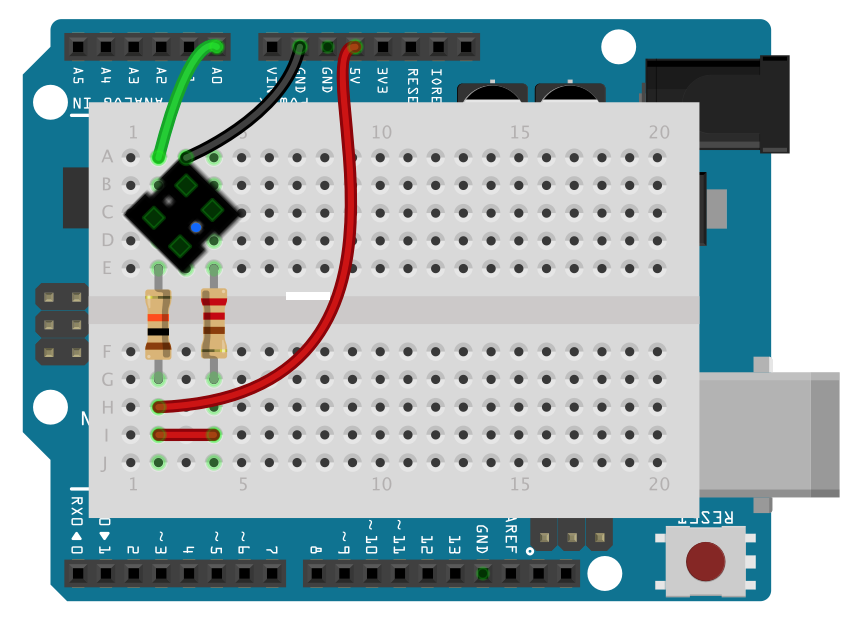
\includegraphics[width=0.45\textwidth]{Kapitel2/Bilder/cny70bb}
\caption{Aufbau der Schaltung}
\label{fig:cny70breadboard}
\end{center}
\end{figure}



\subsection{Aufgaben}
\subsubsection{Aufgabe 1}
In Abb. \ref{fig:cny70breadboard} ist eine funktionierende Schaltung abgebildet. Baue diese Schaltung nach, überprüfe zunächst die Funktion der IR-LED mit Hilfe einer Digitalkamera (z.B. deiner Smartphone-Camera\footnote{Neuere Smartphones funktionieren nicht, da oft die Camera einen guten IR-Filter besitzt}).  Wenn dieser Teil der Schaltung  funktioniert, dann kann die restliche Schaltung aufbauen werden. Achte besonders darauf keinen Kurzschluss zu verursachen und die richtigen Widerstände zu benutzen.

Lade anschließend den Sketch \ref{lst:tcny70} auf den Arduino und überprüfe mit Hilfe der seriellen Schnittstelle die Funktion deiner Schaltung.

\subsubsection{Aufgabe 2}
Um den Sketch voll zu nutzen müsst du deine Schaltung so umbauen, dass die IR-LED über den digitalen PIN 05 mit Spannung versorgt werden kann. 

Untersucht nun den Einfluss des Umgebungslichtes auf deine Messergebnisse. Wie kannst du den Einfluss reduzieren. (Physikalische aber auch programmtechnische Lösungen sind möglich)

\subsubsection{Aufgabe 3}
Versucht mit Hilfe deiner Schaltung eine schwarze Linie zu erkennen, indem du deine Schaltung über das Papier bewegt und die entsprechenden Werte für weißes Papier bzw. schwarze Linie notierst. Wenn du nun mit dem Reflexoptokoppler über eine schwarze Linie fährst, soll eine grüne LED aufleuchten. 


\clearpage


%%%%%%%%%%%%%%%%%%%%%%%%%%%%
%%%  Ultraschall       %%%%%
%%%%%%%%%%%%%%%%%%%%%%%%%%%%
\section{Digitaler Sensor: Der Ultraschallsensor}
\label{sec:ultra}
Ein Ultraschallsensor, wie der ''Seeed Ultrasonic Sensor'' von Seeed oder ''Ping))) Ultrasonic Range Sensorist'' von Parallax soll unser erstes Beispiel für einen digitaler Sensor sein. Wenn du die Rückseite des Sensors anschaust, dann siehst du sehr viel Elektronik und man ahnt schon, dass dieser Sensor wohl anderst funktioniert als z.B. ein Photowiderstand. 
\marginimage{Kapitel2/Bilder/Ping))}

\subsection{Funktionsweise des Ultraschallsensors}

\margininfo{Die Steuerung des Sensors und das Empfangen von Daten über digitale Pins wird auch Protokoll genannt! Im Falle des Ultraschallsensors ist das verwendete Protokoll aber sehr einfach. Das Protokoll, das wahrscheinlich am öftesten verwendet wird ist ``IPv4''. ``IPv4'' regelt LAN oder W-LAN Verbindung zwischen elektronischen Geräten.}

\begin{figure}[h]
\begin{center}
  \begin{tikzpicture}[remember picture]
    % Image 
    \node[anchor=south west,inner sep=0] (image) at (0,0) {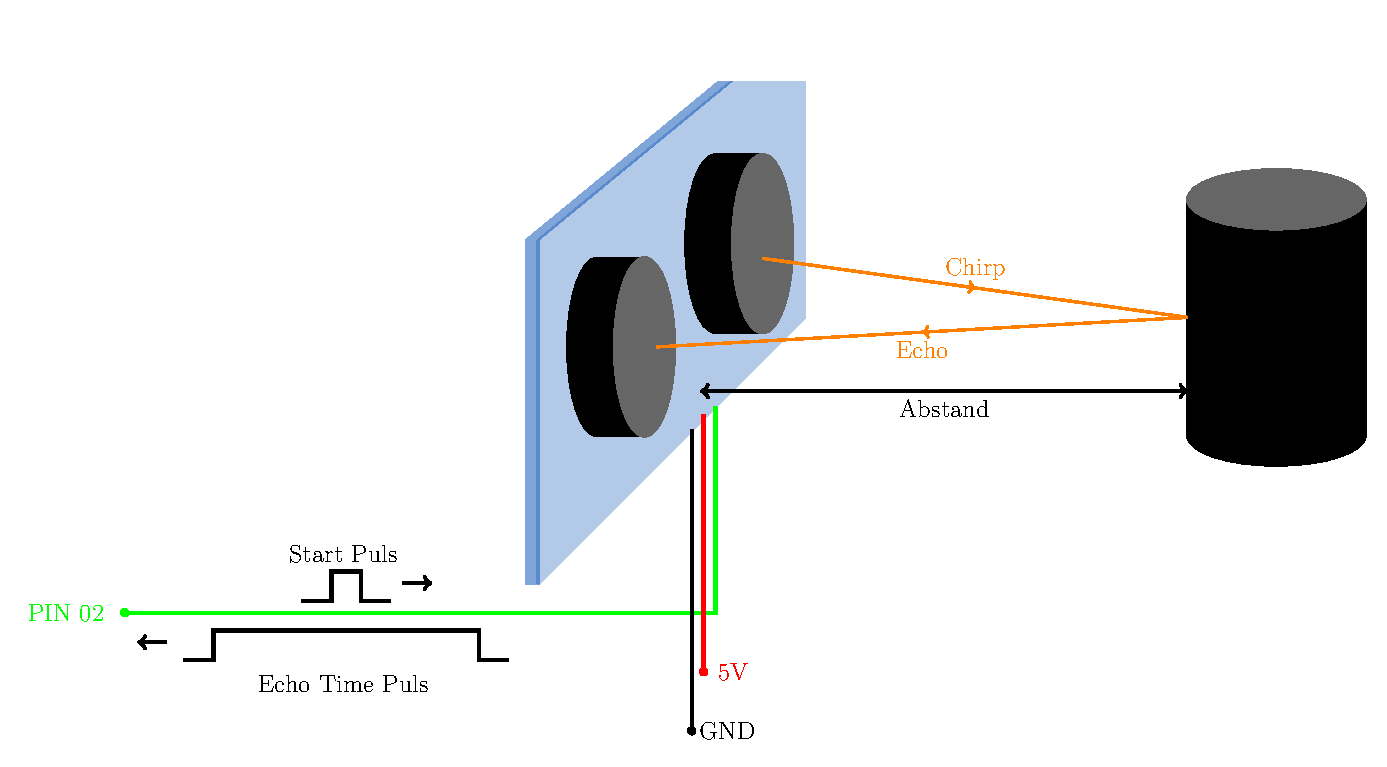
\includegraphics[width=0.9\textwidth]{Kapitel2/Bilder/funktPing}};
    
    % Marks 
    \node (start) at (4.5,3) {};
    \node (sender) at (9.5,6.5) {};
    \node (object) at (15,5.5) {};
    \node (collector) at (8,5) {};
    \node (signal) at (4,0.75) {};
    % comment
    \node[draw=red, fill=red!20, rounded corners,minimum width=0.2\textwidth, minimum height=1.4\baselineskip, anchor=west,align=center,text width=0.3\textwidth] (item1) at (0,4) {Messung wird durch den Startpuls begonnen};
    \node[draw=red, fill=red!20, rounded corners,minimum width=0.2\textwidth, minimum height=1.4\baselineskip, anchor=west,align=center,text width=0.3\textwidth] (item2) at (10,8){Sender: ein kurzer Ultraschall Plus wird ausgesendet};
    \node[draw=red, fill=red!20, rounded corners,minimum width=0.2\textwidth, minimum height=1.4\baselineskip, anchor=west,align=center,text width=0.2\textwidth] (item3) at (14,2.5){Gegenstand: Ultraschallpuls wird reflektiert};
    \node[draw=red, fill=red!20, rounded corners,minimum width=0.2\textwidth, minimum height=1.4\baselineskip, anchor=west,align=center,text width=0.2\textwidth] (item4) at (9.5,1.5){Empfänger: Reflektierter Ultraschallpuls wird erkannt};
    \node[draw=red, fill=red!20, rounded corners,minimum width=0.2\textwidth, minimum height=1.4\baselineskip, anchor=west,align=center,text width=0.4\textwidth] (item5) at (0,-0.5){Signal: Dauer des Antwortpulses entspricht der Flugzeit des Ultraschall Pulses};
    
    \path[red, thick,-] (start.south) edge [out=90 , in=-90] (item1);
    \path[red, thick,-] (sender.east) edge [out=0 , in=-90] (item2);
    \path[red, thick,-] (object.north) edge [out=-10 , in=90] (item3);
    \path[red, thick,-] (collector.north) edge [out=-20 , in=90] (item4);
    \path[red, thick,-] (signal.north) edge [out=-90 , in=90] (item5);
    
    
    \path[red, very thick,-latex'] (item1.north) edge [out=90, in=180](item2.west);
    \path[red, very thick,-latex'] (item2.east) edge [out=0 , in=30] (item3.east);
    \path[red, very thick,-latex']  (item3.south) edge [out=-90, in=0] (item4.east);
    \path[red, very thick,-latex']  (item4.south) edge [out=-90, in=0](item5.east);
    % grid 
    %\draw[color=red,help lines,xstep=1,ystep=1] (0,0) grid (18,8);
    %\draw[help lines,thin,xstep=.5,ystep=.5] (0,0) grid (18,8);
    %\foreach \x in {0,1,...,18} { \node [anchor=north] at (\x,0) {\x}; }
    % \foreach \y in {0,1,...,8} { \node [anchor=east] at (0,\y) {\y}; }  
  \end{tikzpicture}
  \end{center}
  \caption{Funktionsweise eines Untraschallsensors}
  \label{fig:funktPing}
\end{figure}

%Der Ultraschallsensor strahlt zyklisch einen kurzen, hochfrequenten Schallimpuls aus. Dieser pflanzt sich mit Schallgeschwindigkeit in der Luft fort. Trifft er auf ein Objekt, wird er dort reflektiert und gelangt als Echo zurück zum Ultraschallsensor. Aus der Zeitspanne zwischen dem Aussenden des Schallimpulses und dem Empfang des Echosignals berechnet der Ultraschallsensor intern die Entfernung zum Objekt. Da die Entfernung zum Objekt über eine Schall-Laufzeitmessung und nicht über eine Intensitätsmessung bestimmt wird, haben Ultraschallsensoren eine ausgezeichnete Hintergrundausblendung. Ultraschallsensoren erlauben Entfernungsmessungen von 20 mm bis 10 m und können dank der Laufzeitmessung den Messwert mit millimetergenauer Auflösung erfassen. 




\subsection{Beispiel Sketch}

\marginfigure{Kapitel2/Bilder/ping}{Ultraschall Sensor Ping)))}{fig:ping}

\begin{multicols}{2}
\begin{arduinoCode}{Testsketch für einen UltraschallSensor}{lst:ultra}
int pingPin = 2; (*@ \tikzmark{senPin} @*)

void setup() {
  Serial.begin(9600); 
}

void loop() {
  pinMode(pingPin, OUTPUT);  (*@ \tikzmark{output} @*)
  digitalWrite(pingPin, LOW);
  delayMicroseconds(2);
  digitalWrite(pingPin, HIGH); (*@ \tikzmark{startPuls} @*)
  delayMicroseconds(15);
  digitalWrite(pingPin, LOW);
  delayMicroseconds(20);
  
  
  pinMode(pingPin, INPUT);  (*@ \tikzmark{input} @*)
  long cm = pulseIn(pingPin, HIGH)/29/2; (*@ \tikzmark{echoPuls} @*)

  Serial.print(cm);
  Serial.println(" cm");
  
  delay(100);
}
\end{arduinoCode}
\vfill\null 
\columnbreak
\null\vfill 
\begin{itemize}
  \itemsep15pt
  \item[] \tikzmarkcomment{item1}{Digitaler PIN02 ist der Signal-Pin}
  \itemsep50pt
  \item[] \tikzmarkcomment{item2}{PIN02 wird auf ``OUTPUT'' gesetzt}
  \itemsep15pt
  \item[] \tikzmarkcomment{item3}{Start Puls wird gesendet}
  \itemsep25pt
  \item[] \tikzmarkcomment{item4}{PIN02 wird auf ``INPUT'' gesetzt}
  \itemsep35pt
  \item[] \tikzmarkcomment{item5}{Die Pulsdauer wird mit Hilfe der Funktion ``pulsIn()'' gemessen und mit Hilfe der Schallgeschwindigkeit in cm umgerechnet}
  \itemsep15pt
\end{itemize}
\vfill \null

\begin{tikzpicture}[remember picture,overlay]
  \path[red, thick,-] (senPin.east) edge [out=0 , in=180] (item1);
  \path[red, thick,-] (output.east) edge [out=0 , in=180] (item2);
  \path[red, thick,-] (startPuls.east) edge [out=0 , in=180] (item3);
  \path[red, thick,-] (input.east) edge [out=0 , in=180] (item4);
  \path[red, thick,-] (echoPuls.east) edge [out=-20 , in=180] (item5);
\end{tikzpicture}

\end{multicols}

\subsection{Aufgaben}

\margininfo{Um das Datenblatt im Internet zu finden, verwendest du die Suchwörter ``Datasheet'' und die Bezeichnung des Sensors}

Es gibt auch Ultraschallsensoren mit vier Beinchen. Dabei wird ein Pin zum senden des Start Pulses verwendet und der andere zum empfangen des Echo Pulses. Schreibe deinen Sketch so um, dass du den HC-SR04 Sensor verwenden kannst. Diese Sensoren sind um den Faktor fünf billiger als die mit drei Beinchen.
Finde anhand des Datenblattes zu deinem Ultraschallsensor den Messbereich und die Genauigkeit des Ultraschallsensors heraus. Baue dann die Schaltung entsprechend Abb. \ref{fig:ping} oder \ref{fig:hc-sr04} auf. Du muss unbedingt die Bezeichnung der Pins auf dem Sensor beachten, alle  Pins müssen richtig verbunden sein, ansonsten kann der Sensor zerstört werden (und die sind leider teuer).

\subsubsection{Aufgabe 1}
Lade den Sketch aus Listing \ref{lst:ultra} auf deinen Arduino und ändere ihn gegebenenfalls ab. Mach dich mit der Funktion vertraut und überprüfe den Messbereich und die Genauigkeit des Sensors. 

\marginfigure{Kapitel2/Bilder/ping-hc-sr04}{Ultraschall Sensor HC-SR04}{fig:hc-sr04}

                          
\subsubsection{Aufgabe 2}
Bau einen Ultraschallsensor und drei farbige LEDs (grün, gelb und rot) auf dein BreadBoard. Schreibe einen Sketch der einen optischen Abstandsmelder realisiert.

\begin{multicols}{2}
\begin{arduinoCode}{Testsketch "hc-sr04Test.ino" für den HC-SR04}{lst:hc-sr04}
int trigPin = 3; (*@ \tikzmark{trigPin} @*)
int echoPin = 2; (*@ \tikzmark{echoPin} @*)

void setup() { 
  Serial.begin(9600);
  pinMode(trigPin, OUTPUT); 
  pinMode(echoPin, INPUT); 
}

void loop() {
  digitalWrite(trigPin, HIGH); 
  delay(1000);                   (*@ \tikzmark{startPuls} @*)
  digitalWrite(trigPin, LOW);

  long cm = pulseIn(echoPin, HIGH)/29.1/2;(*@ \tikzmark{echoPuls} @*)
}
\end{arduinoCode}
\vfill\null 
\columnbreak
\null\vfill 
\begin{itemize}
  \itemsep15pt
  \item[] \tikzmarkcomment{item1}{Digitaler PIN02 ist der Trigger-Pin}
  \item[] \tikzmarkcomment{item2}{Digitaler PIN02 ist der Echo-Pin}
  \itemsep45pt
  \item[] \tikzmarkcomment{item3}{PIN02 wird auf auf HIGH gesetzt um den Start Puls zu senden}
  \itemsep35pt
  \item[] \tikzmarkcomment{item4}{Die Pulsdauer wird mit Hilfe der Funktion ``pulsIn()'' gemessen und mit Hilfe der Schallgeschwindigkeit in cm umgerechnet}
  \itemsep15pt
\end{itemize}
\vfill \null

\begin{tikzpicture}[remember picture,overlay]
  \path[red, thick,-] (trigPin.east) edge [out=0 , in=180] (item1);
  \path[red, thick,-] (echoPin.east) edge [out=0 , in=180] (item2);
  \path[red, thick,-] (startPuls.east) edge [out=0 , in=180] (item3);
  \path[red, thick,-] (echoPuls.east) edge [out=-20 , in=180] (item4);
\end{tikzpicture}

\end{multicols}

\clearpage

\section{Umwelt Sensoren}
\label{sec:UmweltSensoren}

Es gibt Sensoren, die so komplex sind, dass sie durch ein spezielles Protokoll gesteuert werden müssen. Für diese Sensoren ist dieses Protokoll in einer sogenannten Bibliothek (eng. Library) schon programmiert. Um den Snesor zu Benutzen wird am Anfang des Sketches diese mit Hilfe des Befehls ``\#include "libName.h";'' eingebunden. Dadurch wird der Befehlssatz des Arduino erweitert. Der Kombi-Sensor DH11 ist so ein Sensor. Er verbindet die Temperatur-Messung mit einer Feuchtigkeits-Messung der Luft. Mit Hilfe dieses Sensors kann der Taupunkt indirekt gemessen werden und so z.B. eine intelligente Raumlüftung realisiert werden, die effektive das kondensieren von Wasser an Wänden verhindert und so der Schimmelbindung aktiv entgegenwirkt. 



\marginfigure{Kapitel2/Bilder/dh11test}{Temperatur- und Feuchtigkeits-Sensor DH11}{fig:dh11test}

\subsection{Beispiel Sketch}

\begin{multicols}{2}
\begin{arduinoCode}{Test-Sketch für den DHT 11 Sensor}{lst:dht}
#include "DHT.h" (*@ \tikzmark{loadLib} @*)
          
DHT dht(6, DHT11); (*@ \tikzmark{object} @*)

void setup() {
  Serial.begin(9600); 
  dht.begin(); (*@ \tikzmark{begin} @*)
}

void loop() {
  delay(2000);

  float h = dht.readHumidity(); (*@ \tikzmark{readHumi} @*)
  float t = dht.readTemperature(); (*@ \tikzmark{readTemp} @*)
  
  if (isnan(h) || isnan(t)) { (*@ \tikzmark{check} @*)
    Serial.println("Failed to read!");
  } else {
    Serial.print("H= " + h + " % "); 
    Serial.print("T= " + t + " *C ");
  }  
}
\end{arduinoCode}
\vfill\null 
\columnbreak
\null\vfill 
\begin{itemize}
  \itemsep20pt
  \item[] \tikzmarkcomment{item1}{Zunächst wird die Bibliothek für den Seondor eingebunden}
  \itemsep25pt
  \item[] \tikzmarkcomment{item3}{Ein Sensor ``Objekt'' wird erzeugt}
  \item[] \tikzmarkcomment{item4}{Der Sensor wird gestartet, das dauert bis zu 2 Sekunden}
  \itemsep15pt
  \item[] \tikzmarkcomment{item5}{Das Auslesen der Luftfeuchtigkeit und Temperatur dauert jeweils 0,25 Sekunden! }
  \item[] \tikzmarkcomment{item6}{Ausgabe erfolgt nur, wenn das Lesen geklappt hat}
\end{itemize}
\vfill \null

\begin{tikzpicture}[remember picture,overlay]
  \path[red, thick,-] (loadLib.east) edge [out=0 , in=180] (item1);
  \path[red, thick,-] (object.east) edge [out=0 , in=180] (item3);
  \path[red, thick,-] (begin.east) edge [out=0 , in=180] (item4);
  \path[red, thick,-] (readHumi.east) edge [out=0 , in=180] (item5);
  \path[red, thick,-] (check.east) edge [out=0 , in=180] (item6);
  
\end{tikzpicture}

\end{multicols}

\subsection{Aufgaben}

Baue den DHT11 Sensor auf dem BreadBoard auf und teste deine Schlatung mit Hilfe des Beispielsketches.

\subsubsection{Aufgabe 1}
Schreibe ein Funktion vom Typ float, die als Parameter die Temperatur t und Luftfeuchtigkeit h besitzt und die Taupunkttemperatur $T_p$ berechnet.

\begin{equation}
  T_p = \left(\frac{h}{100}\right)^\frac{1}{8,02}(109,8+t)-109,8
\end{equation}

\begin{arduinoCode}{Taupunkttemperatur ``ttp''}{lst:ttp}
ttp = pow(H/100,1.0/8.02)*(109.8+t)+109.8;
\end{arduinoCode}

Erweitere deinen Sketch, so dass die Taupunkttemperatur berechnet wird und wenn die aktuellen Temperatur kleiner als die Taupunkttemperatur wird eine Warnung über die serielle Schnittstelle versendet wird.
 
\sectionExkurs{Daten Speichern und Auslesen}

\subsection{Die verschiedenen Speicher}
Auf dem Arduino Uno der ATmega328 Microcontroller verbaut. Er besitzt drei Arten von Steuer:
\begin{itemize}
  \item Flash ist der Speicher, in dem der Sketch gespeichert und ausgeführt wird. 
  \item SRAM ist der Speicher, in dem Variablen gespeichert und manipuliert werden können.
  \item EEPROM ist der Speicher, der von Programmen genutzt werden kann um Daten dauerhaft zu speichern.
\end{itemize}


Flash Speicher und  EEPROM Speicher sind nicht flüchtig, das heißt die Daten sind auch nach Stromunterbrechung noch vorhanden. SRAM Speicher ist flüchtig, das heißt die gespeicherten Daten sind nach einer Stromunterbrechung nicht mehr vorhanden. Der ATmega328 IC besitzt folgende Speichergrößen:

\begin{figure}[h]
  \begin{center}
  \tikzset{ 
      table/.style={
          matrix of nodes,
          row sep=-\pgflinewidth,
          column sep=-\pgflinewidth,
          nodes={
              rectangle,
              draw=black,
              align=center
          },
          minimum height=1.5em,
          text depth=0.5ex,
          text height=2ex,
          nodes in empty cells,
  %%
          every even row/.style={
              nodes={fill=gray!20}
          },
          column 1/.style={
              nodes={text width=0.1\textwidth}
          },
          column 2/.style={
              nodes={text width=0.1\textwidth}
          },
          column 3/.style={
              nodes={text width=0.4\textwidth}
          },
          row 1/.style={
              nodes={
                  fill=black!80,
                  text=white,
                  font=\bfseries
              }
          }
      }
  }
  \begin{tikzpicture}
  \matrix (first) [table,text width=6em]
  {   
   Speicher & Größe & Bemerkung \\
   Flash  & 32kB & 0.5kB enthält den Bootloader \\
   SRAM   & 2kB & Speicherbereich für Varaiablen\\
   EEPROM & 1kB & Langzeit Speicher\\
  };
  \end{tikzpicture}
  \caption{Speichergrößen des Arduino Uno}
  \label{tab:speicher}
  \end{center}
\end{figure}
\margininfo{1kB = 1024 Byte \\ B steht für Byte \\ ein Byte besteht aus 8 Bit \\ 1 Bit ist die kleinste Speichergröße}
Es gibt nicht wirklich viel SRAM auf dem Arduino Uno! Bei größeren Datenmengen kann es passieren, dass er vollständig gefüllt wird. Zum Beispiel
\begin{arduinoCode}{}{}
char message[] = "I support the Cape Wind project.";
\end{arduinoCode}
belegt 33 Bytes im SRAM, jedes Zeichen und das Endzeichen '\textbackslash 0' ein Byte.
Dies scheint nicht viel zusein, aber es braucht nicht viel um 2048 Bytes zu füllen. Wenn du den ganzen SRAM aufgebracht hast, kann es zu komischen Fehlern kommen.

Du kannst so eine Sketch oft ohne Fehler auf den Arduino laden, da der SRAM während der Laufzeit gefüllt wird. Wenn der Sketch dann ausgeführt werden soll funktioniert er nicht richtig. Es kommt du komischen Fehlern, die nur sehr schwer zu verstehen sind.

\subsection{EEPROM Speicher benutzen}

\begin{multicols}{2}
\begin{arduinoCode}{EEPROM mit Daten füllen}{lst:eeprom-write}
#include <EEPROM.h> (*@ \tikzmark{lib} @*) 

void setup()
{   (*@ \tikzmark{for} @*) 
  for (int i = 0; i < 255; i++)
    EEPROM.write(i, i); (*@ \tikzmark{write} @*) 
}

void loop()
{
}
\end{arduinoCode}

\vfill
\columnbreak

\null\vfill
\begin{itemize}
  \itemsep15pt
  \item[] \tikzmarkcomment{item1}{EEPROM Library einbinden}
  \item[] \tikzmarkcomment{item2}{for-Schleife}
  \item[] \tikzmarkcomment{item3}{Daten schreiben}
\end{itemize}
\vfill \null

\begin{tikzpicture}[remember picture,overlay]
  \path[red, thick,-] (lib.east) edge [out=0 , in=180] (item1);
  \path[red, thick,-] (for.east) edge [out=5 , in=180] (item2);
  \path[red, thick,-] (write.east) edge [out=0 , in=180] (item3);
\end{tikzpicture}

\end{multicols}


\begin{multicols}{2}
\begin{arduinoCode}{EEPROM mit Daten füllen}{lst:eeprom-write}
#include <EEPROM.h> (*@ \tikzmark{lib} @*) 

int a = 0;
int value;

void setup() {
  Serial.begin(9600);
}

void loop() {
  value = EEPROM.read(a); (*@ \tikzmark{read} @*) 

  Serial.print(a); (*@ \tikzmark{ser} @*) 
  Serial.print(" = ");
  Serial.println(value);
  
  a = a + 1; (*@ \tikzmark{ort} @*) 
  if (a == 256) {
    a = 0;
  }
  delay(500);
}
\end{arduinoCode}

\vfill
\columnbreak

\null\vfill
\begin{itemize}
  \itemsep15pt
  \item[] \tikzmarkcomment{item1}{EEPROM Library einbinden}
  \item[] \tikzmarkcomment{item2}{Daten aus EEPROM lesen}
  \item[] \tikzmarkcomment{item3}{Daten über serielle Schnittstelle an PC übertragen}
  \item[] \tikzmarkcomment{item4}{Leseort um eine Einheit erhöhen}
\end{itemize}
\vfill \null

\begin{tikzpicture}[remember picture,overlay]
  \path[red, thick,-] (lib.east) edge [out=0 , in=180] (item1);
  \path[red, thick,-] (read.east) edge [out=5 , in=180] (item2);
  \path[red, thick,-] (ser.east) edge [out=0 , in=180] (item3);
  \path[red, thick,-] (ort.east) edge [out=0 , in=180] (item4);
\end{tikzpicture}

\end{multicols}


%%%%%%%%%%%%%%%%%%%%%%%%%%%%%%%%%%%%%%%%%%%%%%%%%%%%%%%
%%%  Schleifen %%%%%%%%%%%%%%%%%%%%%%%%%%%%%%%%%%%%%%%%
%%%%%%%%%%%%%%%%%%%%%%%%%%%%%%%%%%%%%%%%%%%%%%%%%%%%%%%
\sectionInformatik{C Sprachstruktur: Schleifen}
Eine Schleife ist eine weitere Kontrollstruktur. Sie dient zur Wiederholung eines Anweisungsblock, den sogenannten Schleifenrumpf oder Schleifenkörper. Dieser wird solange die Schleifenbedingung als Laufbedingung gültig bleibt bzw. die Abbruchbedingung nicht eintritt wiederholt. Schleifen, die keine Schleifenbedingung haben, sind Endlosschleifen. Im Arduino-Sketch stellt die Loop-Methode eine solche Endlosschleife dar.

Prinzipiell können verschiedene Schleifentypen  unterschieden werden:
\begin{itemize}
  \item Die vorprüfende oder kopfgesteuerte Schleife. \\
    Bei dieser Schleife wird eine Bedingung geprüft, mit der vorher entschieden wird, ob der Schleifenkörper ausgeführt wird, diese wird meist als  while-Schleife bezeichnet.
  \item Die nachprüfende oder fußgesteuerte Schleife. \\
    Bei dieser Schleife wird nach dem Durchlauf des Schleifenkörpfers eine Bedingung überprüft, ob der Schleifenrumpf nochmal ausgeführt wird (meist als DO...WHILE = „ausführen...solange“ oder REPEAT...UNTIL = „wiederholen...bis“ Konstrukt).

  \item Die Zählschleife, eine Sonderform der vorprüfenden Schleife (meist als FOR = für -Schleife implementiert). \\
  \item Die Mengenschleife, eine Sonderform der Zählschleife (meist als FOREACH = „für jedes Element der Menge“ implementiert).
  \item Schleife mit Laufbedingung: Wertet die Bedingung zu „wahr“ aus, wird die Schleife fortgesetzt.
    Schleife mit Abbruchbedingung: Wertet die Bedingung zu „wahr“ aus, so wird die Schleife abgebrochen.
\end{itemize}

\marginfigure{Kapitel2/Tikz/out/for.pdf}{for-Loop}{fig:for-loop}

\subsection{for-Schleife: die zählende Wiederholung}

Eine for-Schleife ist eine Kontrollstruktur, mit der man eine Gruppe von Anweisungen, den Schleifenkörper mit einer bestimmten Anzahl von Wiederholungen ausführen kann.
Die Anzahl der Wiederholungen steht schon beim Eintritt in die Schleife fest. Es gibt eine Schleifenvariable, die am Anfang auf den Startwert gesetzt wird und dann jeweils um die Schrittweite verändert wird, bis der Zielwert erreicht ist. Die Schleifenvariable, der Startwert, die Schrittweite und der Endwert müssen numerisch sein. 

\begin{multicols}{2}
\begin{arduinoCode}{Die for-Schleife}{lst:forloop}

        (*@ \tikzmark{ini} @*)               (*@ \tikzmark{test} @*)
for (Initialisieren; Testen; Zaehlen) {
                              (*@ \tikzmark{inc} @*)

 // Anweisungen; (*@ \tikzmark{anw} @*)


}
\end{arduinoCode}

\vfill
\columnbreak

\begin{itemize}
  \itemsep15pt
  \item[] \tikzmarkcomment{item1}{Initialisieren der Schleifenvariablen}
  \item[] \tikzmarkcomment{item2}{Bedingung für die Schleifenvariablen überprüfen.}
  \item[] \tikzmarkcomment{item3}{Schleifenvariablen erhöhen}
  \item[] \tikzmarkcomment{item4}{Anweisungen, die wiederholt ausgeführt werden.}
\end{itemize}


\begin{tikzpicture}[remember picture,overlay]
  \path[red, thick,-] (ini.east) edge [out=35 , in=180] (item1);
  \path[red, thick,-] (test.east) edge [out=20 , in=180] (item2);
  \path[red, thick,-] (inc.east) edge [out=-5 , in=180] (item3);
  \path[red, thick,-] (anw.east) edge [out=-5 , in=180] (item4);
\end{tikzpicture}
\vfill 
\end{multicols}


In C ist die for-Schleife viel flexibler als for-Schleifen in vielen anderen Programmiersprachen, einschließlich BASIC. So kann auf alle der drei Kopfelemente verzichtet werden, nur die Strichpunkte sind nötig. 

 

\clearpage
\subsubsection{Sensorwert in Array speichern und Mittelwert berechnen}

\begin{multicols}{2}
\begin{arduinoCode}{Mittelwert berechnen}{lst:calcMean}
const int senPin = A0;
const int numberOfValues = 10; (*@ \tikzmark{number} @*)
float senValues[numberOfValues]; (*@ \tikzmark{sensorValues} @*) 
float meanValue = 0.0; (*@ \tikzmark{meanValue} @*)

void setup() {
  Serial.begin(9600);
  
}

void loop() {
  for (int i=0;i<numberOfValues;i++) { (*@ \tikzmark{measureLoop} @*)
    senValues[i] = analogRead(senPin);
    delay(20);
  }
  for (int i=0;i<numberOfValues;i++) { (*@ \tikzmark{meanLoop} @*)
     meanValue += senValues[i];
  }
  
  meanValue /= numberOfValues; (*@ \tikzmark{calcMean} @*)
  Serial.println(meanValue);
  delay(200);  
}
\end{arduinoCode}
\vfill
\columnbreak
\null\vfill
\begin{itemize}
  \itemsep25pt
  \item[] \tikzmarkcomment{item1}{Anzahl der Einzelmessungen}
  \item[] \tikzmarkcomment{item2}{Array zur Speicherung der Einzelmessungen}
  \item[] \tikzmarkcomment{item3}{Speicherplatz für gemittelten Sensorwert.}
  \item[] \tikzmarkcomment{item4}{Loop für die Einzelmessungen}
  \item[] \tikzmarkcomment{item5}{Loop für die Mittelwertbildung}
  \item[] \tikzmarkcomment{item6}{Mittelwert berechnen und an PC senden}
\end{itemize}
\vfill \null
\begin{tikzpicture}[remember picture,overlay]
  \path[red, thick,-] (number.east) edge [out=0 , in=180] (item1);
  \path[red, thick,-] (sensorValues.east) edge [out=0 , in=180] (item2);
  \path[red, thick,-] (meanValue.east) edge [out=0 , in=180] (item3);
  \path[red, thick,-] (measureLoop.east) edge [out=0 , in=180] (item4);
  \path[red, thick,-] (meanLoop.east) edge [out=0 , in=180] (item5);  
  \path[red, thick,-] (calcMean.east) edge [out=0 , in=180] (item6);  
\end{tikzpicture}
\end{multicols}

\subsection{Aufgaben}

\subsubsection{Aufgabe 1} 
Schreibe einen Sketch, der die Summe der ganzen Zahlen von 1 bis 10 berechnet. Gib dein Ergebnis über die serielle Schnittstelle aus.


\clearpage 
\subsection{while-Schleife: die bedingte Wiederholung}



\marginfigure{Kapitel2/Tikz/out/while.pdf}{while-Loop}{fig:while-loop}
\begin{multicols}{2}
\begin{arduinoCode}{Die for-Schleife}{lst:forloop}

           (*@ \tikzmark{test} @*)
 while (bedingung) {
   
 // Anweisungen; (*@ \tikzmark{anw} @*)

}
\end{arduinoCode}

\vfill
\columnbreak

\begin{itemize}
  \itemsep15pt
  \item[] \tikzmarkcomment{item1}{Bedingung auf Wahrheit  überprüfen.}
  
  \item[] \tikzmarkcomment{item2}{Anweisungen, die wiederholt ausgeführt werden.}
\end{itemize}


\begin{tikzpicture}[remember picture,overlay]
  \path[red, thick,-] (test.east) edge [out=20 , in=180] (item1);
  \path[red, thick,-] (anw.east) edge [out=-5 , in=180] (item2);
\end{tikzpicture}
\vfill 
\end{multicols}


\subsection{Sprungbefehle}

Möchte man innerhalb einer Schleife (for, do oder while) auf ein Ereignis reagieren, indem die Schleife nicht weiter ausgeführt wird, steht der Befehl break zur Verfügung. Sprungbefehle sollte aber nur dann benutzt werden, wenn es keine andere Lösung gibt (, was praktisch nie der Fall ist).



\begin{multicols}{2}
\begin{arduinoCode}{MVerwendung von break}{lst:break}
for (x = 0; x < 255; x ++)
{
    analogWrite(pwmPin, x);
    sens = analogRead(sensorPin);  
    if (sens > threshold){ 
       x = 0;
       break;  (*@ \tikzmark{break} @*)
    }  
    delay(50);
}
(*@ \tikzmark{cont} @*)

\end{arduinoCode}
\vfill
\columnbreak
\null\vfill
\begin{itemize}
  \itemsep35pt
  \item[] \tikzmarkcomment{item1}{Wenn ein bestimmter Sensorwert überschritten ist, dann wird mit Hilfe des Befehls Break das weiter abarbeiten der for-Schleife unterrochen}
  \item[] \tikzmarkcomment{item2}{und der Sketch nach dem Ende des Schleifenkörpers sortgesetzt}
\end{itemize}
\vfill \null
\begin{tikzpicture}[remember picture,overlay]
  \path[red, thick,-] (break.east) edge [out=0 , in=180] (item1);
  \path[red, thick,-] (cont.east) edge [out=0 , in=180] (item2);  
\end{tikzpicture}
\end{multicols}












% Kapitel 3 %
\chapter{Actoren}

\epigraph{Die Maschine kann nur tun, was wir ihr zu befehlen wissen.}{Ada Lovelace (1815-1852) eigentlich Augusta Ada King Byron, Countess of Lovelace,
britische Mathematikerin }
\minitoc% Creating an actual minitoc
%!TEX root = ../Arduino.tex
%Kapitel 3%
\section{RGB-LEDs}
RGB-LED bestehen aus 3 farbigen (rot, grün und blau) LEDs. Die eine gemeinsame Kathode (Minuspol) besitzen. Sie eignen sich dazu Mischfarben, die aus den drei Grundfarben aufgebaut sind darzustellen. Mit zwei Potentiometer und einem weißen Tischtennisball können schöne Farbeffekte erzeugt werden.      

\marginfigure{Kapitel3/Bilder/rgb-led}{RGB-LED}{fig:rgb-led}

\subsection{Farben mit Potentiometer mischen}

An vielen elektronischen Geräten findet man Regler, an denen man drehen oder schieben kann. Dahinter stecken meistens Potentiometer, kurz „Poti“ genannt. Sie sind regelbare Widerstände und haben meistens drei Anschlüsse. Üblicherweise ist der linke Anschluss an einem Ende einer Kohleschicht befestigt, der rechte Anschluss am anderen Ende. Der mittlere Anschluss, genannt Mittelabgriff, ist mit einem Kontakt verbunden, der auf der Kohleschicht schleift und beim Drehen oder Schieben verschoben wird. Da die Kohlebahn relativ schlecht leitet, fließt ein Strom leichter durch ein kurzes dünnes Stück Kohlespur als durch ein langes ebenso dünnes Stück Kohle. Beim Drehen des Potentiometers wird also der elektrische Widerstand zwischen dem Mittelabgriff und jedem der anderen Anschlüsse verändert. Wenn man Potentiometer kauft, ist meistens der Maximalwiderstand angegeben. Der minimale Widerstand beträgt nahezu $0\Ohm$.

\subsection{Aufbau der Schaltung}
RGB-LEDs sind empfindlich und relativ teuer, das heißt sie dürfen nur mit Vorwiderstand betrieben werden. Wenn du die Schaltung ohne die $220\Ohm$-Widerstände aufbaust bist du schnell um ca. 1 Euro ärmer, aber um eine Kaputte RGB-LED reicher! Ansonsten erfolgt der Aufbau genau wie mit normalen LEDs. Der längste Anschluss ist die gemeinsame Kathode (Minus-Pol) und wird mit GND verbunden. Die anderen Pins werden mit PWM-Ports verbunden.   
\margininfo{Es gibt auch Anoden RGB-LEDs, der gemeinsamme Pin ist dann die Anode (plus Pol).}

\subsection{Aufgaben}

\subsubsection{Aufgabe 1}
Baue zuerst die Schaltung entsprechend Abb. \ref{fig:rgb-led} auf. Öffne den Beispiel-Sketch Beispiele/01Basic/Fade und ändere den Sketch so ab, dass die rote LED über den digitalen PIN 11, die blaue auf dem digitalen PIN 12 und die grüne LED auf dem digitalen PIN 13 angesteuert werden können. 

Ändere für die verschieden Ports den brightness-Wert und versuche so verschiedene Farben zu erzeugen. 

\subsubsection{Aufgabe 2}
Für dieses Aufgabe benötigst du ein größeres Bread-Board. Bau dann die Schaltung entsprechend der Abb. \ref{fig:rgb-mischer} auf. Lade anschließend den Beispiel-Sketch Beispiele/10StarterKit/p04\_ColorMixingLamp. Anstelle der Photo-Widerstände werden bei dieser Aufgabe die Potis verwendet. Mache dich mit der Funktionsweise dieses Sketches vertraut.  

\marginfigure{Kapitel3/Bilder/rgb-mischer}{RGB Mischer}{fig:rgb-mischer} 

\subsubsection{Aufgabe 3 Projekt}
Wenn du die Aufgabe 1 und 2 gut verstanden hast, dann solltest du jetzt in der Lage sein RGB-LED in verschiedenen Projekten zu verwenden. Vielleicht wäre es eine gute Übung für dich dein optisches Thermometer anstatt mit 3 LEDs (rot, gelb und grün) mit einer RGB-LED neu aufzubauen. Eine weitere Idee wäre es eine optische Abstandswarnung zu bauen. Im Abschnitt \ref{sec:farbenraum} ist noch Hintergrundwissen zur Farberzeugung mit Hilfe einer RGB-LED zu finden.     

\subsection{Der Farbenraum}\label{sec:farbenraum}
Ein RGB-Farbraum ist ein additiver Farbraum, der Farbwahrnehmungen durch das additive Mischen dreier Grundfarben (Rot, Grün und Blau) nachbildet. Das Farbsehen des Menschen ist von drei Zapfentypen geprägt. 

Dieser Farbraum wird für selbstleuchtende (farbdarstellende) Systeme benutzt, die dem Prinzip der Additiven Farbmischung unterliegen, daher auch als Lichtmischung bezeichnet. Nach Graßmanns Gesetzen lassen sich Farben durch drei Angaben definieren, im RGB-Farbraum sind dies der Rot-, der Grün- und der Blauanteil. Die konkrete Form des Farbraums hängt vom jeweils konkreten technischen System ab, für das der jeweilige Farbraum bestimmt wurde.


\marginfigure{Kapitel3/Bilder/rgb-color-space}{RGB Farbenraum}{fig:rgb-color-space}



\sectionInformatik{C Sprachelemente: millis() versus delay()}
\label{sec:millis}
Bisher hast du eine LED mit Hilfe der delay()-Funktion ein und ausgeschaltet. Das ist in Ordnung,  solange das Arduino Board nur eine Aufgabe hat. Aber wie sollte mit dem delay()-Befehl folgende Aufgabe löst werden?

\subsubsection{Aufgabe 1}

Baue die Schaltung aus Abbildung \ref{fig:delay-millis} auf. Die rote LED soll blinken (eine Sekunde an, eine Sekunde aus). Die grüne LED leuchten, wenn der Push-Buttom gedrückt ist und nicht leuchten wenn der Push-Buttom losgelassen wird.

\marginfigure{Kapitel3/Bilder/delay_mills.png}{}{fig:delay-millis}

\subsubsection{Lösungs Hinweis}
Um diese Aufgabe zu lösen, muss man das an- und ausschalten der roten LED so steuern, dass der Arduino nicht blockiert wird. Ein mögliche Lösung bietet der millis()-Befehl. Wenn millis() aufgerufen wird, dann gibt er die Zeit in Millisekunden zurück, seit der Arduino das aktuelle Programm ausführt. 

\begin{multicols}{2}
\begin{arduinoCode}{Aufbau einer C-Funktion}{lst:millis}
const int blinkLed = 13;
long time = 0;  (*@ \tikzmark{time} @*)
boolean stateLed = false; (*@\tikzmark{stateLed} @*)

void setup() {                
  pinMode(blinkLed, OUTPUT);
  time = millis();  
}

void loop() {
  if (millis()-time > 1000){ 
    stateLed = !stateLed; (*@\tikzmark{statechange} @*)
    time = millis();
    digitalWrite(blinkLed, stateLed); (*@\tikzmark{statewrite} @*)
  } 
}
\end{arduinoCode}
\columnbreak
\vfill\null 
\begin{itemize}
  \itemsep20pt
    \item[] \tikzmarkcomment{item1}{Aktuelle Ausführzeit des Sketches wird gespichert}
    \item[] \tikzmarkcomment{item2}{Aktueller Zustand der blickLed wird gespeichert}
    \item[] \tikzmarkcomment{item3}{Zustand der blickLed wird nach einer Sekunde geändert}
    \item[] \tikzmarkcomment{item4}{Zustand der blickLed wird übertragen}
 \end{itemize}
\vfill \null

\begin{tikzpicture}[remember picture,overlay]
  \path[red, thick,-] (time.east) edge [out=0 , in=180] (item1);
  \path[red, thick,-] (stateLed.east) edge [out=0 , in=180] (item2);
  \path[red, thick,-] (statechange.east) edge [out=0 , in=180] (item3);
  \path[red, thick,-] (statewrite.east) edge [out=0 , in=180] (item4);
\end{tikzpicture}
\end{multicols}
\margininfo{! ist der Negations-Operator}
Mit Hilfe des Listings \ref{lst:millis} sollte es dir möglich sein Aufgabe 1 zu lösen.

%\subsection{Call Backs}



%%%%%%%%%%%%%%%%%%%%%%%%%%%%%%%%%%%%%%%
%% Lautsprecher %%%%%%%%%%%%%%%%%%%%%%%
%%%%%%%%%%%%%%%%%%%%%%%%%%%%%%%%%%%%%%%
\section{Lautsprecher}

In Kapitel \ref{chapter:1} haben wir zur Visualisierung des digitalen Ausgänge LED`s benutzt.
Statt optischer Ausgaben über LEDs können aber auch akustische Ausgaben erzeugt werden. 
Dazu wird ein Lautsprecher an einen Ausgang des Mikrokontrollers angehängt und schnell ein und 
ausgeschaltet. Dies erzeugt Kräfte in der Spule des Lautsprechers. Diese Kräfte lassen die Membran
im Lautsprecher hin und her schwingen und wir hören die entsprechende Frequenz der 
Membranschwingung als Ton.

\subsection{Lautstärkeregelung mit einem Potentiometer}

Ihr sollt hier ein Potentiometer verwenden, um die Lautstärke des ohnehin recht leisen Tons noch leiser einstellen, bis der Ton schließlich unhörbar leise wird. Dazu muss die Stromstärke im Lautsprecher verringert werden - der zusätzliche veränderbare Widerstand muss also zwischen den Port und den Lautsprecher oder - das ist genau so gut - zwischen den Lautsprecher und den $5\V$ des digitalen Ports geschaltet werden. 

\marginfigure{Kapitel3/Bilder/ton}{Arduino mit Piezolautsprecher}{fig:ton}

\subsection{Aufgaben}

Baue die Schaltung mit dem Lautsprechen entsprechend Abb. \ref{fig:ton} auf. 

\subsubsection{Aufgabe 1}
Für deine ersten Töne genügt es den „Blink“ Sketch entsprechend anpassen. Dazu muss du den Befehl Delay (Millisekunden) durch ein DelayMicroseconds (Microsekunden) ersetzen und auf den Arduino laden. Wenn dein Lautsprechen mit dem richtigen Port verbunden ist solltest du einen konstanten Ton hören.



\subsubsection{Aufgabe 2}
Für die folgende Aufgabe solltest du auf deine Mitschüler Rücksicht nehmen, indem du ein Potentiometer zur Lautstärke-Regelung einbaust. Bau dazu deine Schaltung entsprechend der Abb. \ref{fig:ton-poti} um. 
\marginfigure{Kapitel3/Bilder/ton-poti}{Lautsprecher mit Poti}{fig:ton-poti}   
In der Tabelle \ref{tab:Tonleiter} sind die Frequenzen der Töne einer C-Dur Tonleiter aufgeführt.
\begin{table}[h]

\begin{center}

\tikzset{ 
    table/.style={
        matrix of nodes,
        row sep=-\pgflinewidth,
        column sep=-\pgflinewidth,
        nodes={
            rectangle,
            draw=black,
            align=center
        },
        minimum height=1.5em,
        text depth=0.5ex,
        text height=2ex,
        nodes in empty cells,
%%
        every even row/.style={
            nodes={fill=gray!20}
        },
        column 1/.style={
            nodes={text width=0.5\textwidth}
        },
        row 1/.style={
            nodes={
                fill=black!90,
                text=white,
                font=\bfseries
            }
        }
    }
}

\begin{tikzpicture}
\matrix (first) [table,text width=6em]
{   
  Ton & c & d  & f & g & a \\
  Frequenz ($\Hz$)& 294 & 329 & 349 & 392 & 440 \\
};
 \end{tikzpicture}
\end{center}
\caption{C-Dur Tonleiter mit Frequenzen }
\label{tab:Tonleiter}
\end{table}%
\begin{itemize}
  \item[a)] Berechnen anhand der Werte aus der Tabelle die Perionendauer für die verschiedenen Töne. Um einen Ton jetzt zu erzeugen, muss der digitale Pin jeweils für die Hälfte der Periodendauer 'HIGH' bwz. 'LOW' sein. 
  \item[b)] Schreibe einen Sketch, der das Lied Alle meine Endchen spielt. 
  \item[c)] Schreibe eine C Funktion: \\
  void playTone(int tone, int duration) \\
  Die einen gegebenen Ton 'tone' für eine bestimmte Zeit 'duration' abspielt. Schreibe den Sketch aus Teil b) entsprechend um, dass jetzt diese Funktion verwendet wird. 
\end{itemize}

\subsubsection{Aufgabe 3 Projekt}
 Der Beispiel-Sketch „Examples/Digital/Melody“ macht das ganze etwas eleganter. Lade den Sketch auf dein Board. Wenn das Abspielen klappt, kannst du versuchen die Melodie zu ändern. Dazu muss du allerdings verstanden haben, wie das Beispiel genau funktioniert. 

Wichtig: Du kannst nur die Töne verwenden, die in der Datei pitches.h definiert sind.

\subsection{Zum weiterlese:}
\begin{itemize}
\item \url{http://arduino.cc/en/Tutorial/Tone}
\end{itemize}

\section{Der Transistor als Schalter oder zur  Verstärkung}
\marginfigure{Kapitel3/Bilder/ndet}{Nachbau des ersten Transistors (CC Attribution-Share Alike 3.0 Unported by \href{https://upload.wikimedia.org/wikipedia/commons/6/62/Nachbau_des_ersten_Transistors.jpg}{commons.wikimedia.org})}{}
Ein Transistor ist ein elektronisches Bauelement zum Schalten und Verstärken von elektrischen Signalen, ohne dabei mechanische Bewegungen auszuführen. Transistoren sind die weitaus wichtigsten „aktiven“ Bestandteile elektronischer Schaltungen, welche beispielsweise in der Nachrichtentechnik, der Leistungselektronik und in Computersystemen eingesetzt werden. Besondere Bedeutung haben Transistoren in integrierten Schaltkreisen, was die derzeit weit verbreitete Mikroelektronik ermöglicht.

Es gibt zwei wichtige Gruppen von Transistoren, nämlich Bipolartransistoren und Feldeffekttransistoren (FET).

Der Metall-Oxid-Halbleiter-Feldeffekttransistor (englisch metal-oxide-semiconductor field-effect transistor, MOSFET auch MOS-FET, selten MOST) gehört zu den Feldeffekttransistoren mit isoliertem Gate. Er ist den Metall-Isolator-Halbleiter-Feldeffekttransistoren (MISFET) zuzurechnen. Obwohl heute dotiertes Polysilizium als Gate-Material vorherrscht, wurde die Bezeichnung MOSFET beibehalten. 

\begin{figure}[h]
  \begin{center}
  \subfigure[PinOut: MOSFET und bipolarer Transistor]{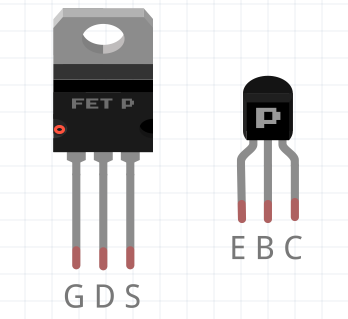
\includegraphics[width=0.3\textwidth]{Kapitel3/Bilder/transistor_pinout}}\qquad\qquad
  \subfigure[Schaltzeichen: MOSFET und bipolarer Transistor]{\begin{circuitikz} %
  \draw (1,3) node[nigfete ](nigfete) {} 
  (nigfete.G)node[anchor=east] {G}
  (nigfete.S)node[anchor=north] {S}
  (nigfete.D)node[anchor=south] {D};
  \draw ($(nigfete)-(0.18,0)$) circle [radius=18pt];
  \draw (4,3) node[npn] (npn) {}
  (npn.base)node[anchor=east] {B}
  (npn.collector)node[anchor=south] {C}
  (npn.emitter)node[anchor=north] {E};
  \draw ($(npn)-(0.18,0)$) circle [radius=18pt]; 
  \draw (0,0) circle; 
  \end{circuitikz}}
  \label{fig:pinout}
  \caption{MOSFET (n-Kanal) und bipolaren Transistor (npn)}
  \end{center}
\end{figure}


\subsection{Einsatzmöglichkeiten für einen bipolaren Transistor}
Grundsätzlich gibt es  zwei verschiedene Möglichkeiten einen bipolaren Transistor zu betreiben:
\begin{itemize}
\item Proportionalbetrieb: Der Kollektor- bzw. Emitterstrom ist proportional zum Basisstrom. Je größer der Basisstrom desto größer der Kollektorstrom. Den Verstärkungsfaktor selbst kannst du im Datenblatt nachlesen. Da die Spannung $U_{CE}$ recht groß ist erwärmt sich der Transistor (Verlustleistung!).
\item Schaltbetrieb: Der Transistor leitet entweder voll oder sperrt komplett. Der Basistrom muss groß genug sein, um den Kollektor- bzw. Emitterstrom nicht zu begrenzen. Ein Basiswiderstand ist für den Schutz des digitalen Ports nötig, nicht für den Betrieb des Transistors. Ohne Basiswiderstand würde der Ausgang des Arduino fast kurzgeschlossen, denn die Vorwärtsspannung U$_{BE}$ ist in der Regel etwa 0,7 V (Achtung: für jeden Transistor muss dieser Wert aus dem Datenblatt entnommen werden). Du benötigst deshalb einen Vorwiderstand von etwa 100$\Ohm$, der den Strom durch den digitalen Port auf maximal $40\mA$ begrenzt.
\end{itemize}

Um die Musik in vernünftiger Lautstärke über einen Lautsprecher auszugeben reicht die maximale zulässige Stromstärke der digitalenPots nicht aus.

\margininfo{Möchte man einen Transistor nur als Schalter verwenden, so ist ein MOSFET einem bipolarem Transistor vorzuziehen, da ein MOSFET praktisch keine Verlustleistung hat.}
\subsection{Aufbau der Schaltung}

Beachte, dass du je nach Transistor im Datenblatt nachsehen musst, wo sich die Basis, der Collector und der Emitter befinden.

\begin{figure}[h]
\begin{center}
\begin{circuitikz}
  \draw (-2,0) node[anchor=east]{GND}
  (4,0) to[short, -o] (-2,0)
  (1,1) node[npn](s2) {} 
  (s2.base) to[R,l=$R_{B}$, -o] ($(s2.base)-(2,0)$)
  ($(s2.base)-(2,0)$) node[anchor=east] {Pin}
  (1,0) to[short, *-]  (s2.south east)
  (1,2) to[short]  (s2.north east)
  (1,2) to[R, l=$R_{Last}$] (1,4)
  (1,4) to[short] (4,4)
  (4,0) to[battery, l=$9V$] (4,4);
  \draw ($(s2)-(0.18,0)$) circle [radius=18pt];\end{circuitikz}
  \caption{Grundschaltung bipolarer Transistor (npn)}
  \label{fig:brueckenschaltung}
\end{center}
\end{figure}

\subsection{Aufgaben}
Baue die Schaltung nach Abb. \ref{fig:ton-npn}. Beachte, dass du für den verwendeten Transistor im Datenblatt nachsehen musst, wo sich die Basis, der Collector und der Emitter befinden.
\marginfigure{Kapitel3/Bilder/ton-npn}{npn-Transistor}{fig:ton-npn}

\subsubsection{Aufgabe 1}
Wenn du dich überzeugt hast, dass die Schaltung richtig aufgebaut ist. Kannst du die Wirkung des bipolaren Transistor und des Potis mit Hilfe deines Melodie-Sketch testen.

\clearpage
\subsection{MOSFET als Schalter}

Auch mit einem MOSFET ist es möglich den Lautsprecher lauter zu bekommen. MOSFET werden dann bevorzugt eingesetzt, wenn die Verlustleistung entscheidend wird.
Da es keine Collector-Source-Strom gibt, ist die Verlustleistung Praktisch Null. Der zweite Einsatz ist wenn sehr große Lasten geschalter werden, so steuert man ein Relais üblicherweise mit einem MOSFET an.

\margininfo{Natürlich kann eine MOSFET auch als Verstärker geschaltet werden. Da es bei ihm keinen Gate-Source-Strom gibt, wird mit Hilfe der Gate-Source-Spannung der Collector-Source-Strom geschaltet. Da aber ohne Spannungsteiler immer $0V$ oder $5V$ Potentialunterschied anliegen, schaltet der MOSFET eben nur.}

\subsection{Aufbau der Schaltung}

\begin{figure}[h]
\begin{center}
\subfigure[Direkte Methode: N-Kanal MOSFET (NFET)\label{fig:nfet}]{ 
 \begin{circuitikz} \draw
(0,0) node[anchor=east]{GND}
  (3,0) to[short, -o] (0,0)
  (1,1) node[nigfete ](s2) {} 
  (s2.G) to[short, o-] (s2.G)
  (s2.G) node[anchor=east] {Pin}
  (1,0) to[short, *-]  (s2.south east)
  (1,2) to[short]  (s2.north east)
  (1,2) to[R, l=$R_{Last}$] (1,4)
  (1,4) to[short] (3,4)
  (3,0) to[battery, l=$9V$] (3,4);
  \draw ($(s2)-(0.18,0)$) circle [radius=18pt];\end{circuitikz}}\qquad 
\subfigure[Direkte Methode: P-Kanal MOSFETs (PFET)\label{fig:pfet}]{ 
 \begin{circuitikz} 
  \draw
  (0,0) node[anchor=east]{GND}
  (3,0) to[short, -o] (0,0)
  (1,1) node[pigfete ](s2) {} 
  (s2.G) to[short, o-] (s2.G)
  (s2.G) node[anchor=east] {Pin}
  (1,0) to[short, *-]  (s2.south east)
  (1,2) to[short]  (s2.north east)
  (1,2) to[R, l=$R_{Last}$] (1,4)
  (1,4) to[short] (3,4)
  (3,0) to[battery, l=$9V$] (3,4);
  \draw ($(s2)-(0.18,0)$) circle [radius=18pt];\end{circuitikz}}
  \caption{Grundschaltung MOSFET}
  \label{fig:brueckenschaltung}
\end{center}
\end{figure}


Zu beachten ist, dass zwischen Gate und Source und zwischen Gate und Drain eine Kapazität existiert, welche bei jedem Umschalt-Vorgang umgeladen werden muss. Besonders bei höheren Frequenzen (größer $ 10\kHz$) ist zur Strombegrenzung zwischen Gate und dem digitalen Port des Arduinos ein Widerstand sinnvoll. Übliche Werte dafür sind $50 - 100\Ohm$. 

\subsection{Aufgaben}
Baue die Schaltung mit dem Lautsprecher und n-MOSFET Transistor entsprechend Abb. \ref{fig:ton-nfet} auf.
\marginfigure{Kapitel3/Bilder/ton-nfet.png}{n-MOSFET Verstärker}{fig:ton-nfet} Anstatt der Batterie wird hier die $5\V$ des Arduino Uno verwendet.   
 
\subsubsection{Aufgabe 1}
Wenn du dich überzeugt hast, dass die Schaltung richtig aufgebaut ist. Kannst du die Wirkung des MOSFETs mit Hilfe deines Melodie-Sketch testen.

\clearpage
\section{Peltier-Element}

Das Peltier- oder thermoelektrische Element, ist  ein Bauteil, das Wärme (Entropie) von einer Seite auf eine andere übertragen kann, wenn ein Strom angelegt wird. Es kann zum heizen oder  kühlen verwenden werden, dazu muss die Stromrichtung umgepolt werden. Das Peltier-Element kann mit zu einer Spannung von $15,4\V$ und einem maximalen Strom von $7A$ versorgt werden.


\subsection{Ausbau der Schaltung}

Du benötigst ein Peltier-Element, einen N-Mosfet,
einen $1000\Ohm$ Widerstand und einen Batteriehalter mit zwei Akkus. Die Abb. \ref{fig:peltier} zeigt den Aufbau der Schaltung.   
\marginfigure{Kapitel3/Bilder/peltier}{Peltier-Element}{fig:peltier}

\subsection{Der Beispiel-Sketch}


\begin{multicols}{2}
\begin{arduinoCode}{Peltier Kühlung}{lst:peltier}
int peltierPin = 3; 
int power = 0; 
int peltLevel = 0; (*@ \tikzmark{init} @*) 

void setup(){
  Serial.begin(9600);
  pinMode(peltierPin, OUTPUT);
}

void loop(){
  if(Serial.available() > 0) {
    int deltaPower = Serial.read();
    power += deltaPower
    peltLevel = map(power, 0, 99, 0, 255);
  }
  Serial.print("Power= ");
  Serial.print(power);
  analogWrite(peltierPin, peltLevel); (*@ \tikzmark{write} @*)
}
\end{arduinoCode}
\columnbreak
\vfill\null 
\begin{itemize}
  \itemsep20pt
    \item[] \tikzmarkcomment{item1}{This is a value from 0 to 255 that actually controls the MOSFET}
    \item[] \tikzmarkcomment{item2}{Write this new value out to the port
}
 \end{itemize}
\vfill \null

\begin{tikzpicture}[remember picture,overlay]
  \path[red, thick,-] (init.east) edge [out=0 , in=180] (item1);
  \path[red, thick,-] (write.east) edge [out=0 , in=180] (item2);
\end{tikzpicture}
\end{multicols}



Das besondere am Sketch aus Listing \ref{lst:peltier} ist, dass das Verhalten des Arduinos über die serielle Schnittstelle gesteuert wird. Man sollte die Schaltung nicht zu lange betreiben, das durch den MOSFET schon einiges an Energie fließt und sich dieser durch die Verlustleistung stark aufheizen kann.


\subsection{Aufgaben}

Bau die Schaltung entsprechend Abb. \ref{fig:peltier} auf. Achte darauf, dass der N-Mosfet richtig eingebaut ist. 
\margininfo{Achtung: Der Mosfet kann bei lagen Betrieb heiß werden!} 

\subsubsection{Aufgabe 1}

Lade den Beispiel-Sketch \ref{lst:peltier} auf deinen Arduino und öffne anschließend das serielle Terminal. Mache dich mit der Funktionsweise des Sketch vertraut und dokumentier alle noch nicht dokumentierten Befehle.

\subsubsection{Aufgabe 2}
Erweitere deine Schaltung und deinen Sketch um einen Temperatur-Sensoren. Messe die Temperatur auf beiden Seiten des Peltier-Elements und gibt die gemessene Temperatur ebenfalls über die serielle Schnittstelle aus.
  
\subsubsection{Aufgabe 3 Projekt}
Erweitere deine Schaltung um ein zweites Peltier-Element das das Heizung geschaltet ist. Erweitere deinen Sketch, so dass eine vorgegebenen Temperatur in einem abgeschlossenen Behälter gehalten werden kann.    


\section{Servomotor}
Soll ein Arduino etwas bewegen, dann gibt es mehrere Möglichkeiten dies zu tun. Es können normale 
Elektromotoren, Schrittmotoren oder Modellbauservos benutzt werden. Modellbauservos haben den 
Vorteil, dass sie leicht anzusteuern sind, und die notwendige Leistungselektronik bereits im Servo 
eingebaut ist. Auch benötigt man keine aufwändigen Rückmeldungen von der Mechanik um eine 
bestimmte Position anzufahren oder um die Schrittverluste eines Schrittmotors auszugleichen. 
Ein Servo findet ganz von alleine nach dem Einschalten seine Neutralposition. 

Servos gibt es in allen möglichen Preiskategorien, wobei die Unterschiede in dem Drehmoment des Motors bzw. in der Qualität des integrierten Getriebes liegen. 

Ein Servo besteht aus mehreren logischen Komponenten

\begin{itemize}
\item Elektronik für die Pulsauswertung
\item Elektronik für eine Regelschleife
\item Leistungselektronik zur Ansteuerung eines Motors
\item der Motor samt Getriebe
\item Positionsauswertung
\end{itemize}
Aus diesen Komponenten wird eine Regelschleife gebildet, so dass der Motor einem 
Positionssignal nachgeführt wird. Am Motor ist ein Getriebe angeflanscht, welches wiederum 
die Abtriebsscheibe bewegt, an der die Bewegung mechanisch abgegriffen werden kann.

\begin{figure}[h]

\centering
\begin{tikzpicture}
[node distance = 1cm, auto,font=\footnotesize,
% STYLES
every node/.style={node distance=3cm, rounded corners},
% The comment style is used to describe the characteristics of each force
comment/.style={rectangle, inner sep= 5pt, text width=4cm, node distance=0.25cm, font=\scriptsize\sffamily},
% The force style is used to draw the forces' name
force/.style={rectangle, draw, fill=black!10, inner sep=5pt, text width=4cm, text badly centered, minimum height=1.2cm, font=\bfseries\footnotesize\sffamily}] 
% arduino
% Draw forces

\node [force, fill=red!20] (arduino) {\large Arduino};


\node [force, right=1cm of arduino] (regelelektronik) {\large Regelelektronik};
\node [force, right=1cm of regelelektronik] (motor) {\large Motor mit Getriebe};
\node [force, fill=blue!20, above=1cm of motor] (rad) {\large Drehung};
\node [force, below of=motor] (position) {\large Positionsbestimmung};

\node[inner sep=0,above=1cm of regelelektronik,text width=3.3cm] (servo) {
   \Large  Servo };
   
\draw [black, fill=gray!50, fill opacity=0.3, dashed]($(regelelektronik.north west)+(-10pt,15pt)$)  -- ($(motor.north east)+(10pt,15pt)$) -- ($(motor.south east)+(10pt,-95pt)$) -- ($(regelelektronik.south west)+ (-10pt,-95pt)$) -- cycle;


%%%%%%%%%%%%%%%
% Change data from here

% ARDUINO
\node [comment, below=0.15cm of arduino] {Versorgung (5Volt und GND) \\ 
Steuerung (digitalPin07)};

%%%%%%%%%%%%%%%%
% Draw the links between forces
\path[->,thick] 
(arduino) edge (regelelektronik)
(regelelektronik) edge (motor)
(motor) edge (position)
(motor) edge  (rad)
(position.west)  edge  [bend left=45] (regelelektronik.south);

\end{tikzpicture} 
\caption{Blockdiagramm eines Servos, der von digitalen Pin07 gesteuert wird}
\label{fig:6forces}
\end{figure}


Der Positionsencoder, im Regelfall ein mechanisch mit dem Getriebe gekoppeltes Potentiometer, 
stellt die Positionsinformation wieder der Regelelektronik zur Verfügung, die bei Abweichungen
entsprechende Motorbewegungen veranlasst. Man gibt also einem Servo nicht eine Bewegung 
vor, sondern eine Position die es ansteuern soll. Die Regelelektronik fährt dann diese Position 
an und hält sie in weiterer Folge.

\subsection{Plusweitenmodulation PWM}

Ein Servo wird mit einem Pulsweiten modulierten Signal (PWM-Signal) angesteuert. Die Information 
über den Winkel ist in der Länge der Pulse enthalten. Der zeitliche Abstand zwischen zwei positiven
Pulsflanken bleibt dabei unverändert. In der Abbildung \ref{fig:pwm} sieht man, wie die Pulsweite 
den Winkel beeinflusst.
\begin{figure}[htbp]
\begin{center}
\subfigure[PWM Signal]{
  \begin{tikzpicture}
    \draw[->] (-0.4,0) -- (6.2,0) node[right] {t in ms};
    \draw[->] (-0.2,-0.2) -- (-0.2,2.6) node[above] {PWM};   
    \draw[] (-.4,2) -- (0,2) node[pos=-0.1, left] {HIGH};
    \draw[] (-.4,0) -- (0,0) node[pos=-0.1, left] {LOW};
     
    \draw[color=red,very thick] plot coordinates {(-0.2,0) (0,0) (0,2)(.2,2) (.2,0) (1,0) (1,2) (1.2,2) (1.2,0) (2,0) (2,2) (2.2,2)(2.2,0) (3,0) (3,2) (3.2,2)(3.2,0) (4,0) (4,2) (4.2,2)(4.2,0) (5,0) (5,2) (5.2,2)(5.2,0) (6,0)};
    
    \draw[|-|,very thick] (1,1) -- (2,1 )
        node[pos=0.7,below]{$t_{pwm}$}; 
    \draw[|-|,very thick] (3,1.1) -- (3.2,1.1 )
        node[pos=2.7,below]{$t_{on}$};     
  \end{tikzpicture}
}

\subfigure[Mittelstellung und maximale Drehung nach links und rechts]{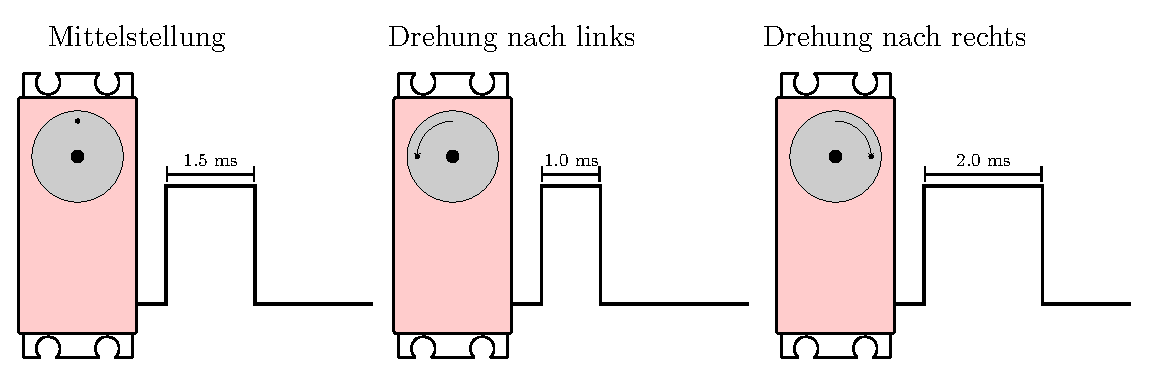
\includegraphics[width=0.9\textwidth]{Kapitel3/Tikz/servoPWM}}

\caption{Der Zusammenhang zwischen Pluslänge des PWM Signals und Drehwinkel des Servus}
\label{fig:pwm}
\end{center}
\end{figure}

Die Zeiten `t periode'' und ``t on'' bestimmen den Servowinkel. In der  Tabelle 
\ref{tab:servopwmtime} stehen die Parameter die von einem Standard-Servo verarbeitet werden. 
Mit diesen Parametern ist ein Servo aber noch nicht vollständig ausgesteuert. Generiert man 
die Signale selber kann man noch mehr Drehwinkel aus dem Servo herausholen. Die maximalen 
Werte müssen für jeden Servotyp experimentell bestimmt werden. Man tut dies, indem man ein 
PWM-Signal generiert das den Servo knapp an den mechanischen Endanschlag stossen lässt. 

\begin{table}[h]

\begin{center}

\tikzset{ 
    table/.style={
        matrix of nodes,
        row sep=-\pgflinewidth,
        column sep=-\pgflinewidth,
        nodes={
            rectangle,
            draw=black,
            align=center
        },
        minimum height=1.5em,
        text depth=0.5ex,
        text height=2ex,
        nodes in empty cells,
%%
        every even row/.style={
            nodes={fill=gray!20}
        },
        column 1/.style={
            nodes={text width=0.5\textwidth}
        },
        row 1/.style={
            nodes={
                fill=black!90,
                text=white,
                font=\bfseries
            }
        }
    }
}
\begin{tikzpicture}
\matrix (first) [table,text width=6em]
{
   Servo Type                             & t periode & t on min & t on max \\
   Standard-Servo                      & 20ms       & 1ms       & 2ms  \\
   Servo Futaba S3003             & 20ms & 0,58ms & 2,4ms \\
   Modellcraft VSD-5E-HS   (digital)    & 10ms &  0,5ms   & 2,3ms \\
};
 \end{tikzpicture}
\end{center}
\caption{Parameter für verschiedene Servos }
\label{tab:servopwmtime}
\end{table}%


\subsection{Aufbau der Schaltung}

Gab es früher je nach Herstellerfirma unterschiedliche Stecksysteme, so hat sich im Laufe der Zeit der
 sog. Uni-Anschluss durchgesetzt. Elektrisch ist der Uni-Stecker so aufgebaut, dass er das in der 
 Elektronik übliche 2.54mm Rastermaß benutzt. Er passt also problemlos auf unser Breadboard.

Dieser Stecker ist mit einem 3-poligen Flachband-Kabel mit der eigentlichen Servoelektronik verbunden.
Gebräuchlich sind einige verschiedene Farbschemen bei diesen Kabeln:

\begin{itemize}
\item schwarz - rot - weiß
\item schwarz - rot - gelb
\item braun - rot - orange
\item schwarz - rot - blau
\end{itemize}

Das schwarz Kabel ist meistens GND und das rot Kabel  die Spannungsversorgung (5Volt). Die dritte Leitung (weiß, gelb, orange, blau, ...) ist die Signalleitung, über die das Servo mit Pulsen versorgt wird, welche ihm die anzufahrende Position mitteilen. Wenigstens in einem Punkt sind sich aber alle Hersteller einig: Die Versorgungsspannung wird immer über die mittlere der 3 Adern des Flachbandkabels geführt, die auch immer rot ausgeführt wird.
\marginfigure{Kapitel3/Bilder/ServoSchaltung_breadboard}{Servomotor}{fig:ServoSchaltung_breadboard}


\subsection{Der Beispielsketch}

Mit dem folgenden Sketch (siehe Listing \ref{lst:servo_simple}) kann ein Servo betrieben werden ohne Hinzunahme von Bibliotheken. Dies kann von Vorteil sein, wenn man Platz auf dem Controller sparen möchte. Es ist hier darauf zu achten, das im folgenden Sketch der digitale Pin07 als Signal Pin für den Servo verwendet wird. Der Servo sollte in diesem Fall also auch entsprechend  angeschlossen sein.

Beim Ausführen des Sketchs bewegt sich der Servo einmal bis zum Anschlag (180 Grad) und dreht wieder zum entgegengesetzten Anschlag zurück. Das Ganze wiederholt sich anschließend.

In der Zeile \ref{lis:servo_postotime} wird die aktuelle Position von Grad in Millisekunden umgerechnet. Dabei entspricht ein Winkel von $0^\circ$ einer PWM-Plusweite von $200\text{ms}$.Ein Winkel von $180^\circ$ einer PWM-Pulsweite von $20\text{ms}$.

\begin{multicols}{2}
\begin{arduinoCode}{PWM Singnal wird erzeugt}{lst:servo_simple}
int servoPin = 3; /
int pwm;  (*@ \tikzmark{pwm} @*) 
int pos; 

void setup() {
   pinMode(servo, OUTPUT);
}

void loop() {
  for(pos=0; pos<180; pos++) {
    servoMove(servoPin, pos); (*@ \tikzmark{servoMove} @*) 
  }
}

void servoMove(int servo, int pos){
  // Winkel in Mikrosekunden umrechnen
  pwm = (pos * 11) + 200; (*@ \label{lis:servo_postotime} @*)  
  digitalWrite(servo, HIGH); (*@ \tikzmark{pwmHigh} @*)
  delayMicroseconds(pwm); // Dauer des PWM-Pluses
  digitalWrite(servo, LOW); // Servo Pin auf LOW Ende des PWM-Pluses
  delay(20); // 20 ms warten
}
\end{arduinoCode}
\columnbreak
\vfill\null 
\begin{itemize}
  \itemsep40pt
    \item[] \tikzmarkcomment{item1}{Mit dem Wert 0 bis 255 wird der Servowinkel gesteuert}
    \item[] \tikzmarkcomment{item2}{Die Funktion servoMove() berechnet aus der Winkelangabe (pos) die Dauer des PWM-Signal  in Millisekunden und erzeugt anschliessend das PWM-Signal. }
    \item[] \tikzmarkcomment{item3}{Servo Pin auf HIGH Beginn des PWM-Pluses}    
 \end{itemize}
\vfill \null

\begin{tikzpicture}[remember picture,overlay]
  \path[red, thick,-] (pwm.east) edge [out=0 , in=180] (item1);
  \path[red, thick,-] (servoMove.east) edge [out=0 , in=180] (item2);
  \path[red, thick,-] (pwmHigh.east) edge [out=0 , in=180] (item3);
\end{tikzpicture}
\end{multicols}

\subsection{Aufgaben}

\subsubsection{Aufgabe 1}
Baue die Schaltung in Abb. \ref{fig:ServoSchaltung_breadboard} nach und teste dann die zwei verschieden Arten (Listing \ref{lst:servo_simple} und \ref{lst:servo2}) einen Servo zu steuern. 
\subsubsection{Aufgabe 2}

Eine etwas einfachere Lösung zeigt Listing \ref{lst:servo2}. Hier wird auf die in der Arduino IDE
 enthaltene Servo Library zurückgegriffen.
 
\subsection{Die Servo Library} %TODO Servo Library fertig schreiben
 Das Beispiel findet sich auch in der IDE unter 
 File $->$ Examples $-> $ Servo.  Achtung: bei Listing \ref{lst:servo2} wird der digitale Pin09 verwendet.

\begin{arduinoCode}{Testsketch für die Servo-Library}{lst:servo2}
#include <Servo.h> 
 
Servo myservo;  // create servo object to control a servo 
                // a maximum of eight servo objects can be created 
 
int pos = 0;    // variable to store the servo position 
 
void setup() 
{ 
  myservo.attach(9);  // attaches the servo on pin 9 to the servo object 
} 
 
 
void loop() 
{ 
  for(pos = 0; pos < 180; pos += 1)  // goes from 0 degrees to 180 degrees 
  {                                  // in steps of 1 degree 
    myservo.write(pos);              // tell servo to go to position in variable 'pos' 
    delay(15);                       // waits 15ms for the servo to reach the position 
  } 
  for(pos = 180; pos>=1; pos-=1)     // goes from 180 degrees to 0 degrees 
  {                                
    myservo.write(pos);              // tell servo to go to position in variable 'pos' 
    delay(15);                       // waits 15ms for the servo to reach the position 
  } 
} 
\end{arduinoCode}

\subsection{Aufgaben}

\subsubsection{Aufgabe 1}


\subsubsection{Aufgabe 2}
Verändere beide Beispiel-Sketche so, dass sich der Servo um $90^\circ$ dreht. Verändere in Listing
\ref{lst:servo_simple} die Zeile \ref{lis:servo_postotime} entsprechend. 

\clearpage
\sectionInformatik{C Sprachstruktur: Library}
%TODO Sprachstruktur Library fertig schreiben

\clearpage
\section{DC-Motoren und externe Spannungsquelle}

DC-Motoren bestehen auf Dauermagneten und Spulen. In der Spule wird beim durchfließen des elektrischen Stromes ein Magnetfeld induziert (erzeugt). Dieses induzierte Magnetfeld und das Magnetfeld des Dauermagneten stoßen einander ab. Durch Schreifkontakte wird der Stromfluss durch die Spule an- bzw. aufgeschaltet. Dadurch entsteht  die Drehung des DC-Motors. Je stärker der Stromfluss ist, desto schneller dreht sich der DC-Motor. Ein normaler DC-Motor benötigt mehr als $100\mA$. Deshalb reicht die max. mögliche Strom der ein digitaler Port ($40mA$) nicht aus um einen DC-Motoren zu betreiben. Mit zwei Motoren kommt man auch schnell an die Grenzen des gesamten Arduino-Boards. Das Arduino-Board (Steuer-Stromkreis) wird deshalb nur als Schalter für einen Externen Stromkreis (Arbeit-Stromkreis) benutzt. Die Steuerung erfolgt mit Hilfe eines n-FET Transistors.   
\marginfigure{Kapitel3/Bilder/dcmotor-nfet}{DC-Motor mit externer Spannungsquelle}{fig:dcmotor-nfet}

\clearpage
\section{Integrierte Schaltkreise, IC}
Viele Schaltungen oder Schaltungsteile kommen in der praktischen Elektronik immer wieder vor. Um 
diese, teilweise komplexen, Schaltungen nicht immer wieder neu aufbauen oder erfinden zu müssen, 
werden sie in integrierte Schaltungen (IS = Integrierter Schaltkreis) zusammengefasst und in einem 
Gehäuse vergossen.

Integrierter Schaltungen sind preisgünstig, da als Massenprodukt gefertigt werden. Durch ihren
kompakten  Aufbau sind die zudem platzsparend und betriebssicher.
 
Vor der Entwicklung integrierter Schaltungen Ende der 1950er wurden elektrische Schaltungen mit 
diskreten Bauteilen aufgebaut, d. h. mit einzelnen Transistoren, Dioden, etc., welche auf einer 
Leiterplatte zu einer Schaltung zusammengefügt wurden. Dies war in Größe und Lebensdauer 
bereits ein wesentlicher Durchbruch gegenüber den damals konkurrierenden Elektronenröhren. 
Die Vorteile durch den Einsatz von Transistoren und Leiterplatten (Platinen), wie Verkleinerung 
und geringere Leistungsaufnahme, verdrängten die Systeme aus Elektronenröhren zunehmend. 
Dieser Trend verstärkte sich mit der Entwicklung und dem massiven Einsatz von integrierten 
Schaltungen ab den 1960ern.

Der erste integrierte Schaltkreis (ein Flipflop) wurde im September 1958 von Jack Kilby entwickelt.
Er bestand aus zwei Bipolartransistoren, welche auf einem Germanium-Substrat befestigt und durch 
Golddrähte verbunden wurden. Dieser Hybrid-Schaltkreis ist somit ein erstes Beispiel der Umsetzung 
der schon bekannten Transistor-Transistor-Logik (TTL) auf einen Schaltkreis. Sie war eine Vorstufe 
zur Weiterentwicklung der TTL-Schaltungen hin zu kleineren Bauformen. Schaltkreise aufgebaut aus 
solchen einfachen integrierten Schaltkreisen steuerten die Apollo Raumschiffe (siehe Abb.\ref{fig:ics3}).

Der erste „monolithische“, d. h. aus bzw. in einem einzigen einkristallinen Substrat gefertigt, 
integrierte Schaltkreis wurde von Robert Noyce im Juli 1959 zum Patent angemeldet. Das 
Entscheidende an Kilbys Erfindung war die komplette Fertigung der Bauelemente und 
Verdrahtung auf einem Substrat. Für die Herstellung wurden bereits fotolithografische 
Verfahren und Diffusionsprozesse genutzt. 

Die ersten integrierten Schaltkreise in Serienproduktion entstanden bereits Anfang der 1960er  
und bestanden lediglich aus bis zu wenigen Dutzend Transistoren (siehe Abb. \ref{fig:ics2}). Mit den Jahren wurden die
Bauelemente jedoch immer weiter verkleinert und auch passive Bauelemente wie Widerstände 
integriert sowie die Komplexität der integrierten Schaltkreise weiter erhöht. Damit erhöhte sich 
auch die Anzahl der Transistoren pro Chip beziehungsweise pro Chip-Fläche, dabei war die 
Anzahl der Transistoren die wichtigste Kenngröße von ICs.

\begin{figure}[htbp]
\begin{center}
\subfigure[IC in DIL/DIP \footnotemark]{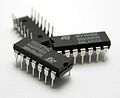
\includegraphics[width=0.3\textwidth]{Kapitel3/Bilder/ic_three}}
\subfigure[TI SN5451, der erste kommerzielle IC \label{fig:ics2}]{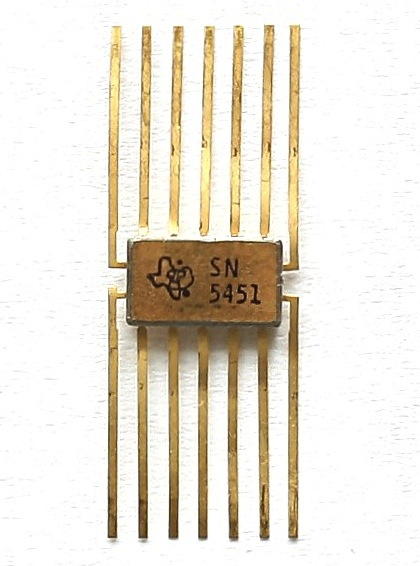
\includegraphics[height=0.3\textwidth, angle=90]{Kapitel3/Bilder/KL_TI_SN5451_Logic_IC}}
\subfigure[Logisches NOR: IC aus dem PC, der das Apollo Raumschiff steuerte \label{fig:ics3}\footnotemark]{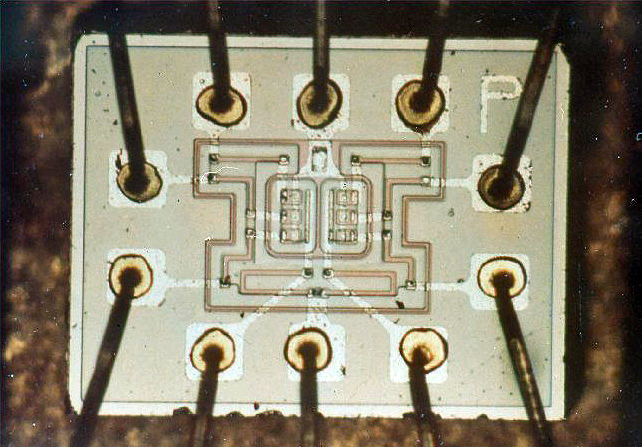
\includegraphics[width=0.28\textwidth]{Kapitel3/Bilder/Agc_nor2}}
\caption{IC im Gehäuse, der erste kommerzielle IC und der erste funktionsfähige IC}
\label{fig:ics}
\end{center}
\end{figure}
\addtocounter{footnote}{-1}\footnotetext{Dual In-Line (DIL), Gehäuse mit Anschlüssen an zwei Seiten, meist im Raster 2,54 mm (=100 mil), die „Urform“ der Chipgehäuse}
\addtocounter{footnote}{1}\footnotetext{Quelle: \url{http://www.ti.com/corp/docs/kilbyctr/downloadphotos.shtml}}

%\section{Shift Register und Ringzähler}
%
%\subsection{Shift Register}
%
%
%\subsection{Ringzähler}
%Der IC 4014 ist ein sogenannter Ringzähler. Er hat 10 Ausgänge. Bei jedem neuen Takt-Impuls am Clock-Eingang wird der nächste Ausgang auf HIGH gesetzt. 
%
%\marginfigure{Kapitel3/Bilder/shift-register}{Shift Register}{fig:shift-register}
%
%
%Die Beschaltung des ICs ist etwas verwirrend, aber man kann die Details ja im Datenblatt (erhältlich z.B. bei Conrad) nachlesen. Der Schalt-Impuls wird vom Arduino auf dem Digitalen Port 2 ausgegeben, indem dieser kurzzeitig auf HIGH und dann wieder auf LOW geschaltet wird. Der Arduino bezieht seinen Strom aus dem angeschlossenem USB-Kabel. Die Schaltung wird mit GND und 5V vom Arduino versorgt. An die Ausgänge des ICs werden 180 Ohm Widerstände und daran LEDs angeschlossen.
%
%\subsection{Der Arduino Sketch}
%
%
%
%
%\subsection{Aufgaben}
%
%\subsubsection{Aufgabe 1}
%Baue die Schaltung für das Shift-Register nach Abb. \ref{fig:shift-register} auf. 
%
%\subsubsection{Aufgabe 2}


\section{Der IC L293D zur Motorsteuerung}
\marginfigure{Kapitel3/Bilder/IC_L293D}{IC L293D}{fig:l293d}

\subsection{Die Brückenschaltung}

Wenn bei einem  DC-Motor die Laufrichtung umgekehrt werden soll, so muss die Richtung des 
elektrischen Stroms der den Motor durchfließt umgekehrt werden. Der einfachste Weg dies zu 
erreichen ist eine sogenannte H-Brückenschaltung. In der Abb. \ref{fig:brueckenschaltung} ist 
schematisch eine H-Brückenschaltung mit vier Schaltern dargestellt. 

\begin{figure}[h]
\begin{center}
\subfigure[Brückenschaltung]{ 
 \begin{circuitikz}
 
 \draw (1,-3) node[anchor=east]{GND} to[short, o-*] (2,-3) ;
 \draw (2,-3) to [-] (6,-3);
 
 \draw (2,-3) to[switch, l=$s_2$] (2,-1);
\draw (2,-1) to[switch, l=$s_1$] (2,1);

\draw (2,-1) to [R, l=$M$, *-*]   (6,-1);

 \draw (6,-3) to[switch, l=$s_4$] (6,-1);
\draw (6,-1) to[switch, l=$s_3$] (6,1);

 \draw (1,1) node[anchor=east]{$V_{dd}$} to[short, o-*] (2,1);
 \draw (2,1) to [-] (6,1);
 
\end{circuitikz}
}
\subfigure[vereinfachte Brückenschaltung mit FETs\label{fig:brueckenschaltung_d}]{ 
 \begin{circuitikz}
 
 \draw (1,-3) node[anchor=east]{GND} to[short, o-*] (2,-3) ;
 \draw (2,-3) to [-] (6,-3);
 
 \draw (2,-2) node[nmos](s2) {}
 	(s2.G)node[anchor=east] {pin02};
\path[-,thick]  (2,-3) edge  (s2.south east);
\draw (2,0) node[nmos](s1) {}
	(s1.G)node[anchor=east] {pin01};
\path[-,thick]  (s1.south east) edge  (s2.north east);
\path[-,thick]  (s1.north east) edge  (2,1);
\draw (2,-1) to [R, l=$M$, *-*]   (6,-1);


 \draw (6,-2) node[nmos](s4) {}
 	(s4.G)node[anchor=east] {pin04};
\path[-,thick]  (6,-3) edge  (s4.south east);	
\draw (6,0) node[nmos](s3) {}
	(s3.G)node[anchor=east] {pin03};
\path[-,thick]  (s3.south east) edge  (s4.north east);
\path[-,thick]  (s3.north east) edge  (6,1);

 \draw (1,1) node[anchor=east]{$V_{dd}$} to[short, o-*] (2,1);
 \draw (2,1) to [-] (6,1);
 
\end{circuitikz}
}
\subfigure[Moter dreht sich rechts herum]{ 
 \begin{circuitikz}
 
 \draw[color=red] (1,-3) node[anchor=east]{GND} to[short, o-*, i_<=$I$] (2,-3) ;
 \draw (2,-3) to [short] (6,-3);
 
 \draw[color=red] (2,-3) to [short, l=$s_2$, i_<=$I$,color=red]  (2,-1);
\draw (2,-1) to[switch, l=$s_1$] (2,1);

\draw[color=red] (2,-1) to [R, l=$M$,i<=$I$,*-*]   (6,-1);

 \draw (6,-3) to[switch, l=$s_4$] (6,-1);
\draw[color=red] (6,-1) to [short, l=$s_3$, i_<=$I$] (6,1);

 \draw[color=red] (1,1) node[anchor=east]{$V_{dd}$} to[short, o-*, i_>=$I$] (2,1);
 \draw[color=red] (2,1) to [short,  i_>=$I$] (6,1);
 
\end{circuitikz}
}
\subfigure[Moter dreht sich rechts herum]{ 
 \begin{circuitikz}
 
 \draw[color=red] (1,-3) node[anchor=east]{GND} to[short, o-*, i_<=$I$] (2,-3) ;
 \draw[color=red] (2,-3) to [short,  i_<=$I$] (6,-3);
 
 \draw(2,-3) to [switch, l=$s_2$] (2,-1);
\draw[color=red]  (2,-1) to [short, l=$s_1$, i_<=$I$,color=red]  (2,1);

\draw[color=red] (2,-1) to [R, l=$M$,i>=$I$,*-*]   (6,-1);

 \draw[color=red]  (6,-3) to [short, l=$s_4$, i_<=$I$]  (6,-1);
\draw (6,-1) to [switch, l=$s_3$] (6,1);

 \draw[color=red] (1,1) node[anchor=east]{$V_{dd}$} to[short, o-*, i_>=$I$] (2,1);
 \draw (2,1) to [short] (6,1);
 
\end{circuitikz}
}


  \caption{Brückenschaltung mit vier Schalter bzw. vier FET-Transistoren}
\label{fig:brueckenschaltung}
\end{center}
\end{figure}

\begin{table}[h]
\begin{center}
\tikzset{ 
    table/.style={
        matrix of nodes,
        row sep=-\pgflinewidth,
        column sep=-\pgflinewidth,
        nodes={
            rectangle,
            draw=black,
            align=center
        },
        minimum height=1.5em,
        text depth=0.5ex,
        text height=2ex,
        nodes in empty cells,
%%
        every even row/.style={
            nodes={fill=gray!20}
        },
        %column 1/.style={
          %  nodes={text width=2em,font=\bfseries}
        %},
        row 1/.style={
            nodes={
                fill=black!90,
                text=white,
                font=\bfseries
            }
        }
    }
}
\begin{tikzpicture}
\matrix (first) [table,text width=6em]
{
	$s_1$ & $s_2$ & $s_3$ & $s_4$ & Verhalten \\
	auf & auf & auf & auf & stop  \\
	auf & zu  & zu  & auf & links  \\
	zu  & auf & auf & zu  & rechts  \\
	zu  & zu  & auf & auf & Kurzschluss  \\
	auf & auf & zu  & zu  & Kurzschluss  \\
};
\end{tikzpicture}
\end{center}
\caption{Mögliche Schaltereinstellungen bei der Brückenschaltung }
\label{tab:brueckenschaltung}
\end{table}%
In der Tabelle \ref{tab:brueckenschaltung} sind die möglichen Schalterstellungen und das 
entsprechende Verhalten des Motors aufgelistet. Wenn nun diese vier Schalter durch 
FET-Transistoren ersetzt werden, ist den möglich mit Hilfe von vier digitalen Pins, die 
jeweils über einen Spannungsteiler mit dem Gate-Eingang der FETs verbunden werden 
eine H-Brückenschaltung zu realisieren, bei der mit Hilfe der digitalen Pins mit Motordrehrichtung 
gesteuert werden kann (vergleiche Abb. \ref{fig:brueckenschaltung_d}).     


\clearpage
\subsection{Pinbelegung des IC L293D}

Zum Glück müssen wir eine Brückenschaltung wie sie Abb. \ref{fig:brueckenschaltung_d}
ohne Spannungsteiler für jeden digitalen Pin zeigt nicht selber aufbauen. Diese Schaltung 
werden in ICs realisiert. Es gibt viele verschiedene Modelle und Marken von H-Bridge-ICs. 
Wir verwenden den IC L293D. Der L293D ist relative billig und ist ohne zusätzliche Kurzschluss-Dioden verwendbar. Deshalb ist er sehr einfach zu benutzen. In der Abb. \ref{fig:l293d1}
ist die Pinbelegung dargestellt. 

\marginfigure{Kapitel3/Bilder/L293D}{Pin Belegung}{fig:l293d1}
\marginfigure{Kapitel3/Bilder/IC_L293D}{IC L293D}{fig:l293d1-bauteil}
 
%\begin{figure}[h]
%\begin{center}
%\subfigure[Pin Belegung\label{fig:l293d1} ]{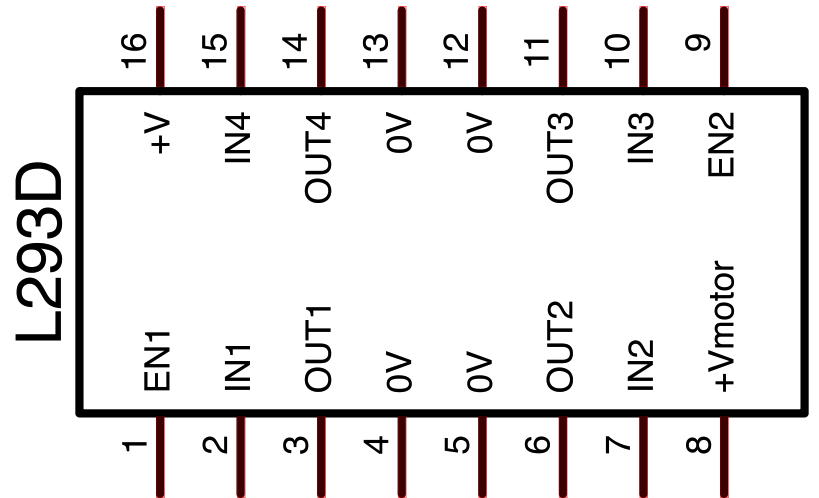
\includegraphics[width=0.45\textwidth]{Kapitel3/Bilder/L293D}}
%\subfigure[Bauteil]{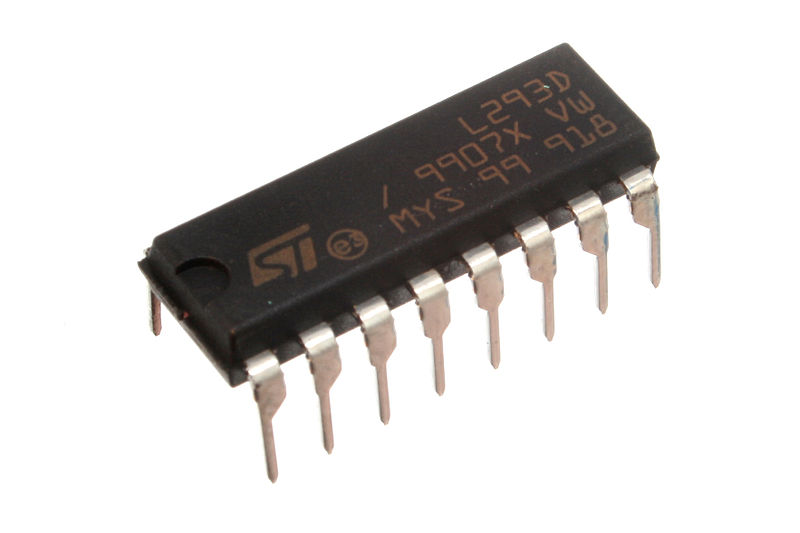
\includegraphics[width=0.45\textwidth]{Kapitel3/Bilder/IC_L293D}}
%\caption{Die Pin Belegung und Aussehen des IC L293D}
%\label{fig:l293d}
%\end{center}
%\end{figure}


\begin{table}
\begin{center}
\tikzset{ 
    table/.style={
        matrix of nodes,
        row sep=-\pgflinewidth,
        column sep=-\pgflinewidth,
        nodes={
            rectangle,
            draw=black,
            align=center
        },
        minimum height=1.5em,
        text depth=0.5ex,
        text height=2ex,
        nodes in empty cells,
%%
        every even row/.style={
            nodes={fill=gray!20}
        },
        column 1/.style={
            nodes={text width=2.2em}
        },
       column 2/.style={
            nodes={text width=2.2em}
        },
       column 3/.style={
            nodes={text width=4em}
        },	
        column 6/.style={
            nodes={text width=0.4\textwidth}
        },
        row 1/.style={
            nodes={
                fill=black!90,
                text=white,
                font=\bfseries
            }
        },
        row 6/.style={
            nodes={text depth=3.5ex}
        }
  }
}
\begin{tikzpicture}
\matrix (first) [table,text width=6em]
{

``IN1'' & ``IN2''	& ``EN1'' & ``OUT1'' & ``OUT2'' & entspricht \\
0V &	 0V	&  5V &   - &  - & Motor kurzschließen (Bremsen)\\
0V &	 5V	& 5V	 &  -  & + & Motor dreht vorwärts\\
5V &	 0V	& 5V	 & +	& -  & Motor dreht rückwärts\\
5V &	 5V	& 5V	 & +  & + &Motor kurzschließen (Bremsen)\\
egal	& egal & 0V & hochohmig & hochohmig & Motor aus (Verbindung trennen, nicht kurzschließen)\\
};
\end{tikzpicture}
\end{center}
\caption{Übersicht der Pinbelegung für einen Motor (1,2) analog für Motor (3,4).}
\label{tab:brueckenschaltung}
\end{table}%

\clearpage
\subsection{Die Schaltung auf dem BreadBoard}
Das schwierige bei der Schaltung für den IC L293D ist, dass sie übersichtlich aufgebaut 
werden muss. In der Abb. \ref{fig:l293d} ist ein mögliche Aufbau dieser für zwei Motoren 
abgebildet. 

\marginfigure{Kapitel3/Bilder/L293D_breadboard}{L293D als Treiber für zwei DC-Motoren}{fig:l293d}


\subsection{Der Beispielsketch}
\begin{multicols}{2}
\begin{arduinoCode}{Testsketch für einen DC-Motor}{lst:dc-motor}
  const int motorPin1 = 5;  // IN1 (*@\tikzmark{inPin} @*)
  const int motorPin2 = 6;  // IN2
    
  void setup() {
    pinMode(motorPin1, OUTPUT); 
    pinMode(motorPin2, OUTPUT); 
  }

  void loop() {
    digitalWrite(motorPin1, HIGH); (*@\tikzmark{rueckwaerts} @*)
    digitalWrite(motorPin2, LOW);  
    delay(3000);
    
    digitalWrite(motorPin1, LOW);  (*@\tikzmark{stopp1} @*)
    digitalWrite(motorPin2, HIGH);
    delay(3000);
    
    digitalWrite(motorPin1, HIGH);  (*@\tikzmark{vorwaerts} @*)
    digitalWrite(motorPin2, LOW);  
    delay(3000);
    
    digitalWrite(motorPin1, LOW);  (*@\tikzmark{stopp2} @*)
    digitalWrite(motorPin2, LOW);
   }
\end{arduinoCode}

\columnbreak
\vfill\null 
\begin{itemize}
  \itemsep20pt
    \item[] \tikzmarkcomment{item1}{Die Motor PINs, wichtig ist, dass PWM-fähige PINs verwendet werden.}
    \item[] \tikzmarkcomment{item2}{Motor dreht sich rückwärts}
    \item[] \tikzmarkcomment{item3}{Motor stoppt}
    \item[] \tikzmarkcomment{item4}{Motor dreht sich vorwärts}
    \item[] \tikzmarkcomment{item5}{Motor stoppt}
 \end{itemize}
\vfill \null

\begin{tikzpicture}[remember picture,overlay]
  \path[red, thick,-] (inPin.east) edge [out=0 , in=180] (item1);
  \path[red, thick,-] (rueckwaerts.east) edge [out=0 , in=180] (item2);
  \path[red, thick,-] (stopp1.east) edge [out=0 , in=180] (item3);
  \path[red, thick,-] (vorwaerts.east) edge [out=0 , in=180] (item4);
  \path[red, thick,-] (stopp2.east) edge [out=0 , in=180] (item5);
\end{tikzpicture}
\end{multicols}

\subsection{Aufgaben}
Bau die Schaltung entsprechend Abb. \ref{fig:l293d} auf. Lade anschließend den Beispiel-Sketch \ref{lst:dc-motor} auf deinen Arduino.

\subsubsection{Aufgabe 1}
Verringere nun die Drehzahl deines Motors mit Hilfe eines PWM-Signals. Dazu musst du die digitalWrite-Befehle durch analogWrite ersetzen.
\margininfo{\textbf{Syntax:}\\
analogWrite(pin, value) \\
\textbf{Parameters:}\\
pin: the pin to write to.\\
value: the duty cycle: between 0 (always off) and 255 (always on). }

\subsubsection{Aufgabe 2}
Entwickle für die die drei verschiedene Zustände des Motor Routinen motorBackward, motorStop und motorForward. Übergabe Parameter sollen die PINs mit denen der Motor verbunden ist und ein PWM-Signal sein. 
\begin{arduinoCode}{}{}
void motorBackward(pin1,pin2,pwm) {
  // Code
}
\end{arduinoCode}

\subsubsection{Aufgabe 3 (Projekt)}
Im Beispiel-Sketch habe dich den Befehl delay() benutzt um den Motor eine definierte Zeit zu bewegen. Bau auf deinem Breadboard noch einen Push-Button hinzu und verwende die Methode aus Kapitel \ref{sec:millis}. Wenn der Push-Button gedrückt wird, soll der Motor stoppen. 


%\clearpage
%\section{Projekt: Deine eigene Motor Library}
%
%\subsection{Funktionsumfang der Library}
%
%\begin{multicols}{2}
%
%\begin{arduinoCode}{Testsketch für einen DC-Motor}{lst:motorlib1}
%
%// Use this code to test your motor with the Arduino board:
%
%// if you need PWM, just use the PWM outputs on the Arduino
%// and instead of digitalWrite, you should use the analogWrite command
%
%//  Motors
%int motor_left[] = {2, 3};
%int motor_right[] = {7, 8};
%
%//  Setup
%void setup() {
%  Serial.begin(9600);
%
%  // Setup motors
%  int i;
%  for(i = 0; i < 2; i++){
%    pinMode(motor_left[i], OUTPUT);
%    pinMode(motor_right[i], OUTPUT);
%  }
%}
%\end{arduinoCode}
%
%\begin{arduinoCode}{Testsketch für einen DC-Motor}{lst:motorlib2}
%//  Loop
%void loop() { 
%
%  drive_forward();
%  delay(1000);
%  motor_stop();
%  Serial.println("1");
%
%  drive_backward();
%  delay(1000);
%  motor_stop();
%  Serial.println("2");
%
%  turn_left();
%  delay(1000);
%  motor_stop();
%  Serial.println("3");
%
%  turn_right();
%  delay(1000);
%  motor_stop();
%  Serial.println("4"); 
%
%  motor_stop();
%  delay(1000);
%  motor_stop();
%  Serial.println("5");
%}
%
%\end{arduinoCode}
%
%
%\begin{arduinoCode}{Testsketch für einen DC-Motor}{lst:motorlib3}
%//  Drive
%
%void motor_stop(){
%  digitalWrite(motor_left[0], LOW); 
%  digitalWrite(motor_left[1], LOW); 
%
%  digitalWrite(motor_right[0], LOW); 
%  digitalWrite(motor_right[1], LOW);
%  delay(25);
%}
%
%void drive_forward(){
%  digitalWrite(motor_left[0], HIGH); 
%  digitalWrite(motor_left[1], LOW); 
%
%  digitalWrite(motor_right[0], HIGH); 
%  digitalWrite(motor_right[1], LOW); 
%}
%
%void drive_backward(){
%  digitalWrite(motor_left[0], LOW); 
%  digitalWrite(motor_left[1], HIGH); 
%
%  digitalWrite(motor_right[0], LOW); 
%  digitalWrite(motor_right[1], HIGH); 
%}
%  
%void turn_left(){
%  digitalWrite(motor_left[0], LOW); 
%  digitalWrite(motor_left[1], HIGH); 
%
%  digitalWrite(motor_right[0], HIGH); 
%  digitalWrite(motor_right[1], LOW);
%}
%
%void turn_right(){
%  digitalWrite(motor_left[0], HIGH); 
%  digitalWrite(motor_left[1], LOW); 
%
%  digitalWrite(motor_right[0], LOW); 
%  digitalWrite(motor_right[1], HIGH); 
%}
%\end{arduinoCode}
%\end{multicols}
%\clearpage

%%%%%%%%%%%%%%%%%%%%%%%%%%%%%%%%%%%%%
%%% Schrittmotoren %%%%%%%%%%%%%%%%%%
%%%%%%%%%%%%%%%%%%%%%%%%%%%%%%%%%%%%%
\section{Schrittmotoren} 
%TODO Schrittmotoren Schaltbild und Schaltung 


Bisher haben wir sog. Gleichstrom-Motoren verwendet. Wird  ein Gleichstrom-Motor mit einer passenden Betriebsspannung versorgt, so fängt er sich sofort an zu drehen. Die Drehzahl hängt dabei von der Leistung der Spannungsversorgung ab. Wenn ein Batterie zum Betrieb verwendet wird dreht sich der Motor langsamer, wenn die Batterie langsam leer wird. Bei spielen Einsatzbereichen ist aber eine genaue Kontrolle der Bewegung nötig.     


Um einen Schrittmotor zu steuern benötigst du ebenfalls  ein Treiber-Chip. Hier kann auch der L293D verwendet werden.

\subsection{Funktionsweise eines Schrittmotors}


\subsubsection{Beispiel-Sketch}
\begin{multicols}{2}
\null\vfill 
\begin{arduinoCode}{Testsketch für einen DC-Motor}{lst:dc-motor}

#include <Stepper.h> (*@\tikzmark{stepperLib}@*)
 
#define STEPS 100 (*@\tikzmark{steps}@*)
 
Stepper stepper(STEPS, 8, 9, 10, 11); (*@\tikzmark{stepperPins}@*)
 
int previous = 0;
 
void setup(){
  stepper.setSpeed(30);  (*@\tikzmark{speed}@*)
}
 
void loop(){
  int val = analogRead(0); (*@\tikzmark{sensor}@*)
  stepper.step(val - previous); (*@\tikzmark{move}@*)
  previous = val;
}
\end{arduinoCode}
  \vfill\null 
  \columnbreak
  \vfill\null 
  \begin{itemize}
    \itemsep15pt
    \item[] \tikzmarkcomment{item1}{Die Stepper Bibliothek wird eingebunden}
    \item[] \tikzmarkcomment{item2}{Anzahl der Schritte pro Umdrehung wird definiert}
    \itemsep25pt
    \item[] \tikzmarkcomment{item3}{Ein Objekt  Stepper wird erzeugt und mit den PINs verbunden}
    \item[] \tikzmarkcomment{item4}{Setzt die Rotationsgeschwindigkeit auf Umdrehungen pro Minute}
    \item[] \tikzmarkcomment{item5}{Sensorwert zur Drehung des Motor wird gemessen (Potentiometer)}
    \item[] \tikzmarkcomment{item6}{Der Stepper wird je nach Messwertwert gedreht.}
 \end{itemize}
\vfill \null

\begin{tikzpicture}[remember picture,overlay]
  \path[red, thick,-] (stepperLib.east) edge [out=0 , in=180] (item1);
  \path[red, thick,-] (steps.east) edge [out=0 , in=180] (item2);
  \path[red, thick,-] (stepperPins.east) edge [out=0 , in=180] (item3);
  \path[red, thick,-] (speed.east) edge [out=0 , in=180] (item4);
  
  \path[red, thick,-] (sensor.east) edge [out=0 , in=180] (item5);
  \path[red, thick,-] (move.east) edge [out=0 , in=180] (item6);
\end{tikzpicture}
\end{multicols}


\subsection{Schrittmotor mit dem Motortreiber A4988}

Wesentlich Komfortabler geht es mit Hilfe des Schrittmotor Treibers A4988 und der zugehörigen Library.  





\marginfigure{Kapitel3/Bilder/nema17A4988.png}{nema 17}{fig:nema17A4988}



%%%%%%%%%%%%%%%%%%%%%%%%%%%%%%%%%%%%%
%%% LCD-Displays %%%%%%%%%%%%%%%%%%%%
%%%%%%%%%%%%%%%%%%%%%%%%%%%%%%%%%%%%%
\section{Display}
%TODO Besser digitales Display  


\marginfigure{Kapitel3/Bilder/LCD.png}{LCD}{fig:lcd}


\subsection{Der Beispiel-Sketch}
\begin{multicols}{2}
\null \vfill
\begin{arduinoCode}{LCD-Display}{lst:lcd}
#include <LiquidCrystal.h> (*@\tikzmark{liqLib}@*)

LiquidCrystal lcd(12, 11, 5, 4, 3, 2); (*@\tikzmark{pins}@*)

void setup() {
  lcd.begin(16, 2); (*@\tikzmark{setCols}@*)
  // 
  lcd.print("hello, world!");(*@\tikzmark{hello}@*)
}

void loop() {
  lcd.setCursor(0, 1); (*@\tikzmark{setPos}@*)
  // :
  lcd.print(millis()/1000); (*@\tikzmark{printMes}@*)
}
\end{arduinoCode}
\vfill\null 
\columnbreak

\begin{itemize}
  \itemsep15pt
    \item[] \tikzmarkcomment{item1}{Die LiquidCrystal Bibliothek wird eingebunden}
    \item[] \tikzmarkcomment{item2}{PINs für das LCD-Displayplay}
    \item[] \tikzmarkcomment{item3}{Setup des LCD's  mit Anzahl der Spalten und Zeilen.}
    \itemsep20pt
    \item[] \tikzmarkcomment{item4}{Schreibt eine Nachricht auf das LCD.}
    \itemsep25pt
    \item[] \tikzmarkcomment{item5}{Setzt den Cursor auf die 0. Spalten in der 1. Zeile. (Beachte: Zeilen und Spalten werden von 0 an gezählt).}
    \itemsep35pt
    \item[] \tikzmarkcomment{item6}{Schreibt die Anzahl der Sekunden seit dem letzten 'reset' auf das Display.}
 \end{itemize}
\vfill \null

\begin{tikzpicture}[remember picture,overlay]
  \path[red, thick,-] (liqLib.east) edge [out=0 , in=180] (item1);
  \path[red, thick,-] (pins.east) edge [out=0 , in=180] (item2);
  \path[red, thick,-] (setCols.east) edge [out=0 , in=180] (item3);
  \path[red, thick,-] (hello.east) edge [out=0 , in=180] (item4);
  
  \path[red, thick,-] (setPos.east) edge [out=0 , in=180] (item5);
  \path[red, thick,-] (printMes.east) edge [out=0 , in=180] (item6);
\end{tikzpicture}
\end{multicols}







% Kapitel 4 %
\chapter{Projekte mit dem Arduino}

\epigraph{Design is not just what it looks like and feels like. Design is how it works}{Steven „Steve“ Paul Jobs (24. Februar 1955 - 5. Oktober 2011), US-amerikanischer Unternehmer}
\epigraph{Don't undertake a project unless it is manifestly important and nearly impossible}{Edwin Herbert Land, (May 7, 1909 – March 1, 1991), American scientist and inventor}
% !TEX TS-program = pdflatex
% !TEX encoding = UTF-8 Unicode

\section{Projektmanagement}



\section{Das optische Tee-Tassen-Thermometer ($oT^3$)}

\subsection{Anforderungen}

\begin{table}[h]

\begin{center}
\tikzset{ 
    table/.style={
        matrix of nodes,
        row sep=-\pgflinewidth,
        column sep=-\pgflinewidth,
        nodes={
            rectangle,
            draw=black,
            align=center
        },
        minimum height=1.5em,
        text depth=0.5ex,
        text height=2ex,
        nodes in empty cells,
%%
        every even row/.style={
            nodes={fill=gray!20}
        },
        column 1/.style={
            nodes={text width=0.5\textwidth}
        },
        row 1/.style={
            nodes={
                fill=black!90,
                text=white,
                font=\bfseries
            }
        }
    }
}

\begin{tikzpicture}
\matrix (first) [table,text width=6em]
{
   Anforderungen   & leicht & mittel & schwer \\
   Schaltung           &       &        &   \\
   Programm          &       &        &   \\
   Aufbau                &       &       &    \\
};
 \end{tikzpicture}
\end{center}
\caption{}
\label{tab:}
\end{table}%



\section{Das eigene Motor Arduino Shield}

\subsection{Anforderungen}
\begin{table}[h]

\begin{center}

\tikzset{ 
    table/.style={
        matrix of nodes,
        row sep=-\pgflinewidth,
        column sep=-\pgflinewidth,
        nodes={
            rectangle,
            draw=black,
            align=center
        },
        minimum height=1.5em,
        text depth=0.5ex,
        text height=2ex,
        nodes in empty cells,
%%
        every even row/.style={
            nodes={fill=gray!20}
        },
        column 1/.style={
            nodes={text width=0.5\textwidth}
        },
        row 1/.style={
            nodes={
                fill=black!90,
                text=white,
                font=\bfseries
            }
        }
    }
}

\begin{tikzpicture}
\matrix (first) [table,text width=6em]
{
   Anforderungen   & leicht & mittel & schwer \\
   Schaltung           &       &        &   \\
   Programm          &       &        &   \\
   Aufbau                &       &       &    \\
};
 \end{tikzpicture}
\end{center}
\caption{}
\label{tab:}
\end{table}%

\subsection{Projektbeschreibung}

\section{SchulBot ein autonomes Fahrzeug}

\subsection{Anforderungen}
\begin{table}[h]
 \begin{center}
  \tikzset{ 
    table/.style={
        matrix of nodes,
        row sep=-\pgflinewidth,
        column sep=-\pgflinewidth,
        nodes={
            rectangle,
            draw=black,
            align=center
        },
        minimum height=1.5em,
        text depth=0.5ex,
        text height=2ex,
        nodes in empty cells,
%%
        every even row/.style={
            nodes={fill=gray!20}
        },
        column 1/.style={
            nodes={text width=0.5\textwidth}
        },
        row 1/.style={
            nodes={
                fill=black!90,
                text=white,
                font=\bfseries
            }
        }
    }
}

  \begin{tikzpicture}
\matrix (first) [table,text width=6em]
{
   Anforderungen   & leicht & mittel & schwer \\
   Schaltung           &       &        &   \\
   Programm          &       &        &   \\
   Aufbau                &       &       &    \\
};
 \end{tikzpicture}
\end{center}
\caption{}
\label{tab:}
\end{table}%

\subsection{Projektbeschreibung}
Teilautonom oder autonom gesteuerte Fahrzeug spielen eine immer größer werdende Rolle in unsere modernen Gesellschaft. In moderne Autos steuern Mikrocontroller Fahrerassistenzsysteme wie z.B. ABS. Diese Technik wird zur Zeit weiterentwickelt. Im Mai 2012 erhielt Google die erste Zulassung eines autonomen Fahrzeugs in den USA. So erlaubte der US-Bundesstaat Nevada den Test des selbstfahrenden Autos auf öffentlichen Straßen. Bedingung ist jedoch, dass sich eine Person hinter dem Steuer befindet, die notfalls eingreifen kann.
\marginfigure{Kapitel4/Bilder/Google_driverless_car}{Google autonomous car}{fig:google_driverless_car}

Im Bereich der Transportfahrzeuge gibt es schon seit längerem automatisierte fahrerlose Fahrzeuge. Fahrerlose Transportsysteme (FTS) sind innerbetriebliche, flurgebundene Fördersysteme mit automatisch gesteuerten Fahrzeugen, deren primäre Aufgabe der Materialtransport, nicht aber der Personentransport ist. Sie werden innerhalb und außerhalb von Gebäuden eingesetzt und bestehen im Wesentlichen aus folgenden Komponenten: 
\begin{itemize}
\item einem oder mehreren Fahrerlosen Transportfahrzeugen
\item einer Leitsteuerung
\item Einrichtungen zur Standortbestimmung und Lageerfassung
\item Einrichtungen zur Datenübertragung
\item Infrastruktur und peripheren Einrichtungen.
\end{itemize}
\marginfigure{Kapitel4/Bilder/Unterfahrschlepper-FTF}{Fahrerlose Transportsystem als Unterfahrschlepper}{fig:ftf}


\subsection{Aufgabenstellung}

Ihr sollte ein autonomes Roboterfahrzeug planen, bauen und programmieren. 
Das Fahrzeug soll folgende Aufgaben lösen.  

\subsubsection{Aufgabe 1}
Das Fahrzeug soll mindestens 10 Meter gerade aus fahren und dabei maximal 1 Meter nach links 
oder rechts abweichen.

\subsubsection{Aufgabe 2}
Euer Fahrzeug soll mit Hilfe zweier Schalter Wände erkennen und dieses Ausweichen. 

\subsubsection{Aufgabe 3}
Euer Fahrzeug soll mit Hilfe eines Optokopplers eine schwarze Linie erkennen und dieser folgen. 


\subsection{Material}

Vorgefertigter Bauplan, zwei Getriebemotoren, Arduino Uno mit ProjektShield, Batteriehalter, 
Grundplatte  

\subsubsection{Fertigungstechniken}
CNC Fräsen, Löte, 


\subsection{Erstellung des Bauplans}

Mit Hilfe der CAD/CAM Software nccad plant und entwerft ihr auf Grundlage der Vorlage 
mcgbot.cad die Bodenplatte eures Fahrzeuges. 

\begin{figure}[htbp]
\begin{center}
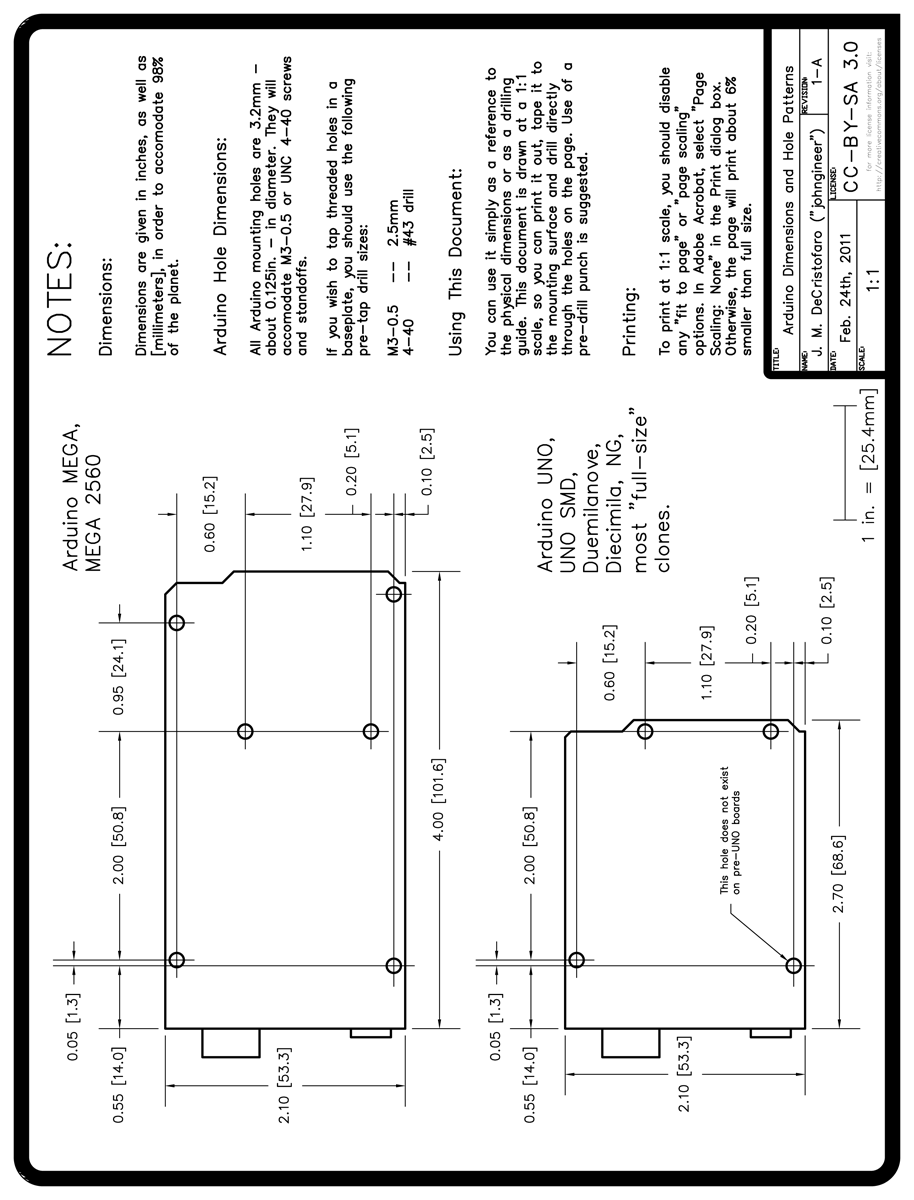
\includegraphics[width=0.7\textwidth,angle=-90]{Kapitel4/Bilder/arduino_dimension}
\caption{default}
\label{default}
\end{center}
\end{figure}


\section{Paperduino-UNO, das selbstgebaute Arduino-Board}

\subsection{Anforderungnen}

\begin{table}[h]

\begin{center}
\tikzset{ 
    table/.style={
        matrix of nodes,
        row sep=-\pgflinewidth,
        column sep=-\pgflinewidth,
        nodes={
            rectangle,
            draw=black,
            align=center
        },
        minimum height=1.5em,
        text depth=0.5ex,
        text height=2ex,
        nodes in empty cells,
%%
        every even row/.style={
            nodes={fill=gray!20}
        },
        column 1/.style={
            nodes={text width=0.5\textwidth}
        },
        row 1/.style={
            nodes={
                fill=black!90,
                text=white,
                font=\bfseries
            }
        }
    }
}

\begin{tikzpicture}
\matrix (first) [table,text width=6em]
{
   Anforderungen   & leicht & mittel & schwer \\
   Schaltung           &       &        &   \\
   Programm          &       &        &   \\
   Aufbau                &       &       &    \\
};
 \end{tikzpicture}
\end{center}
\caption{}
\label{tab:}
\end{table}%

\subsection{Projektbeschreibung}

\begin{figure}[htbp]
\begin{center}
\subfigure[Schaltplan]{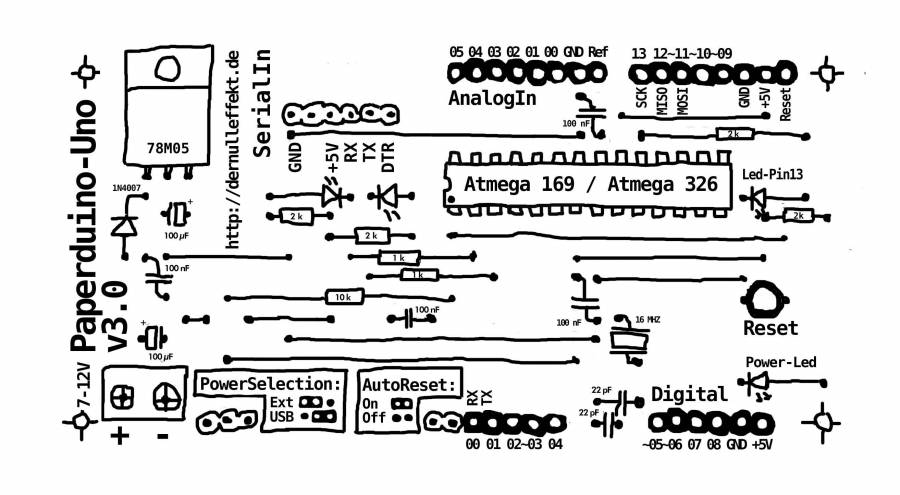
\includegraphics[width=0.4\textwidth]{Kapitel4/Bilder/Paperduino-Uno_30}}
\subfigure[Fertige Platine]{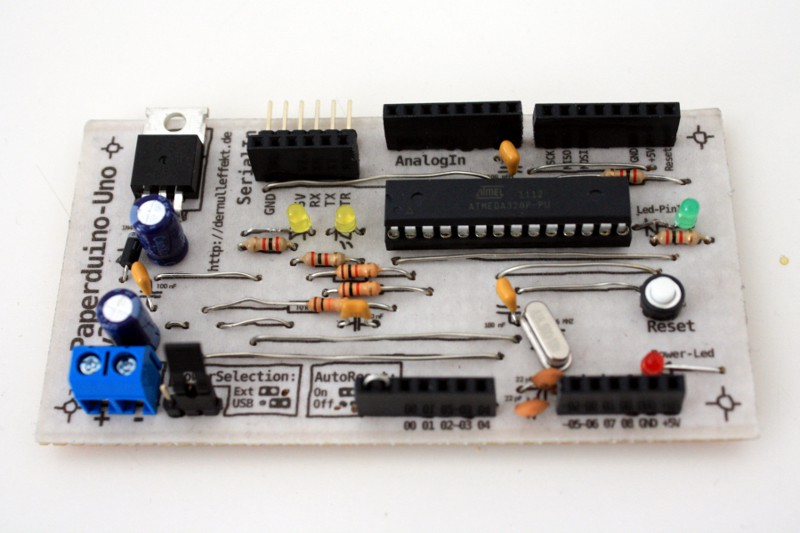
\includegraphics[width=0.4\textwidth]{Kapitel4/Bilder/paperduino-uno-30}}
\caption{default}
\label{default}
\end{center}
\end{figure}


\section{Roboter Arm}

\subsection{Anforderungnen}

\begin{table}[h]

\begin{center}
\tikzset{ 
    table/.style={
        matrix of nodes,
        row sep=-\pgflinewidth,
        column sep=-\pgflinewidth,
        nodes={
            rectangle,
            draw=black,
            align=center
        },
        minimum height=1.5em,
        text depth=0.5ex,
        text height=2ex,
        nodes in empty cells,
%%
        every even row/.style={
            nodes={fill=gray!20}
        },
        column 1/.style={
            nodes={text width=0.5\textwidth}
        },
        row 1/.style={
            nodes={
                fill=black!90,
                text=white,
                font=\bfseries
            }
        }
    }
}

\begin{tikzpicture}
\matrix (first) [table,text width=6em]
{
   Anforderungen   & leicht & mittel & schwer \\
   Schaltung           &       &        &   \\
   Programm          &       &        &   \\
   Aufbau                &       &       &    \\
};
 \end{tikzpicture}
\end{center}
\caption{}
\label{tab:}
\end{table}%

\subsection{Projektbeschreibung}

% Kapitel 5 % 
\chapter{Die Stationskarten}

\epigraph{.}{.}

\minitoc% Creating an actual minitoc

\section*{Stationskarte: \ref{sec:kommunikation} \nameref{sec:kommunikation}}

\margininfo{}
\begin{multicols}{2}
\subsection*{Material-Liste}
\begin{itemize}
  \item Arduino Uno mit Breadboard
  \item Pushbottum
  \item Widerstand (10k$\Ohm$)
\end{itemize}


\vfill\null 
\columnbreak

\subsection*{Versuchsaufbau}

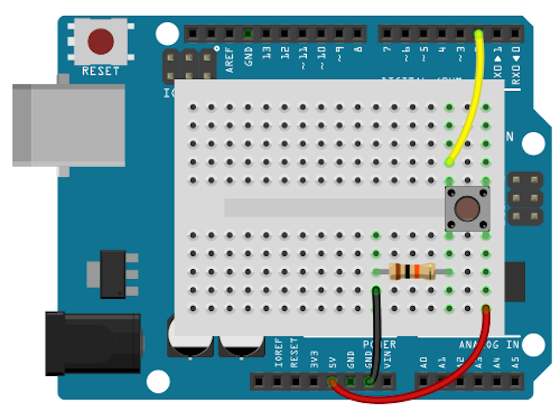
\includegraphics[width=0.5\textwidth]{Kapitel1/Bilder/digitalreadserial2}
\end{multicols}




\section*{Stationskarte: \ref{sec:lm35} \nameref{sec:lm35}}

\margininfo{Achte darauf, dass du den LM35 richtig einbaust. Sollte er sich erwärmen, musst du die Stromversorgung zum Arduino sofort unterbrechen, und den Aufbau deiner Schaltung überprüfen!}
\begin{multicols}{2}
\subsection*{Material-Liste}
\begin{itemize}
  \item Arduino Uno mit Breadboard
  \item Temperatur Sensor LM35
  \item 3 Projekt-Kabel
\end{itemize}


\vfill\null 
\columnbreak

\subsection*{Versuchsaufbau}

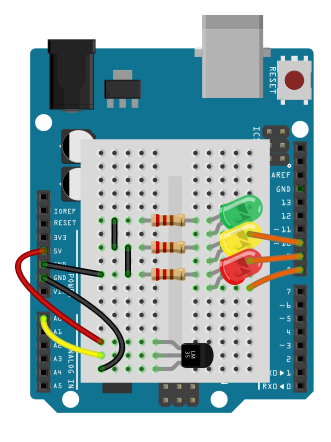
\includegraphics[width=0.5\textwidth]{Kapitel2/Bilder/temperatursensor}
\end{multicols}


\section*{Stationskarte: \ref{sec:lichtsensoren} \nameref{sec:lichtsensoren}}

\margininfo{}
\begin{multicols}{2}
\subsection*{Material-Liste}
\begin{itemize}
  \item Arduino Uno mit Breadboard
  \item LDR (Photozelle)
  \item Widerstand (muss bestimmt werden)
  \item Multimeter
  \item 3 Projekt-Kabel
\end{itemize}

\subsection*{Übersicht Material}

\vfill\null 
\columnbreak

\subsection*{Versuchsaufbau}

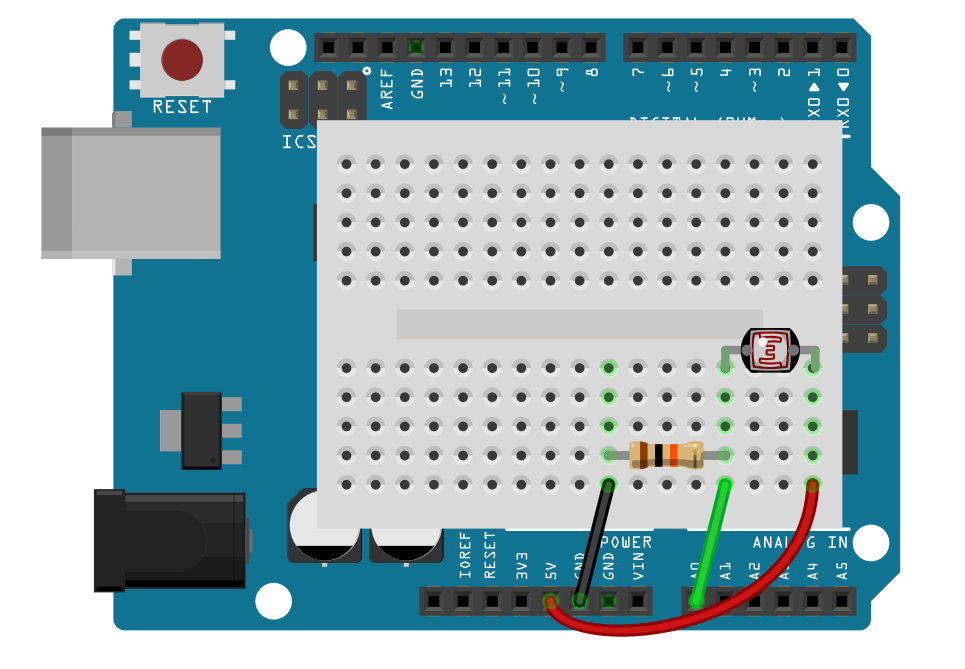
\includegraphics[width=0.5\textwidth]{Kapitel2/Bilder/LDR_bb}
\end{multicols}

\section*{Stationskarte: \ref{sec:reflex} \nameref{sec:reflex}}

\margininfo{}
\begin{multicols}{2}
\subsection*{Material-Liste}
\begin{itemize}
  \item Arduino Uno mit Breadboard
  \item cny70 (Reflexoptokoppler)
  \item Widerstände ($220\Ohm$ und $10k\Ohm$)
  \item 3 Projekt-Kabel
\end{itemize}

\subsection*{Übersicht Material}

\vfill\null 
\columnbreak

\subsection*{Versuchsaufbau}

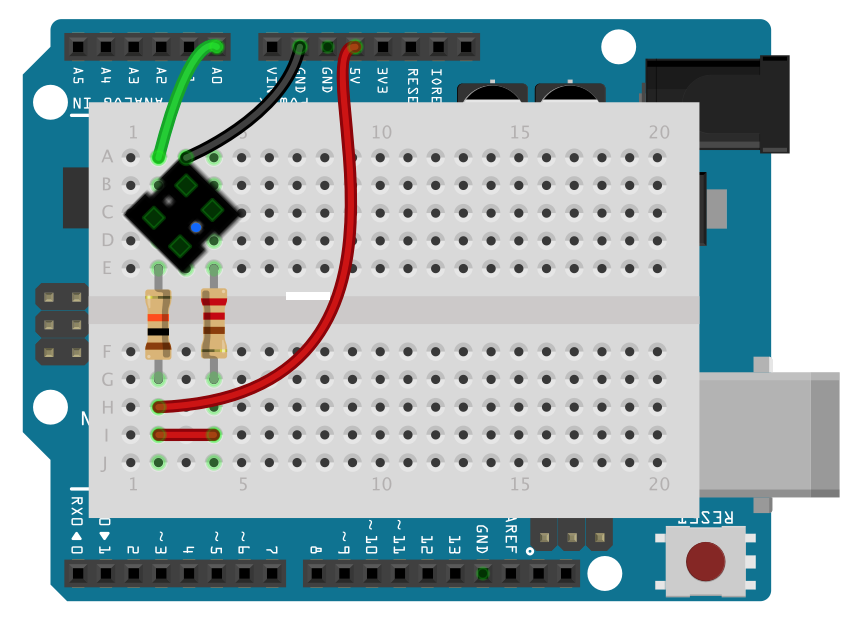
\includegraphics[width=0.5\textwidth]{Kapitel2/Bilder/cny70bb}
\end{multicols}


\section*{Stationskarte: \ref{sec:ultra} \nameref{sec:ultra}}

\margininfo{}
\begin{multicols}{2}
\subsection*{Material-Liste}
\begin{itemize}
  \item Arduino Uno mit Breadboard
  \item Untraschall Sensor
  \item 3 Projekt-Kabel
\end{itemize}

\subsection*{Übersicht Material}

\vfill\null 
\columnbreak

\subsection*{Versuchsaufbau}

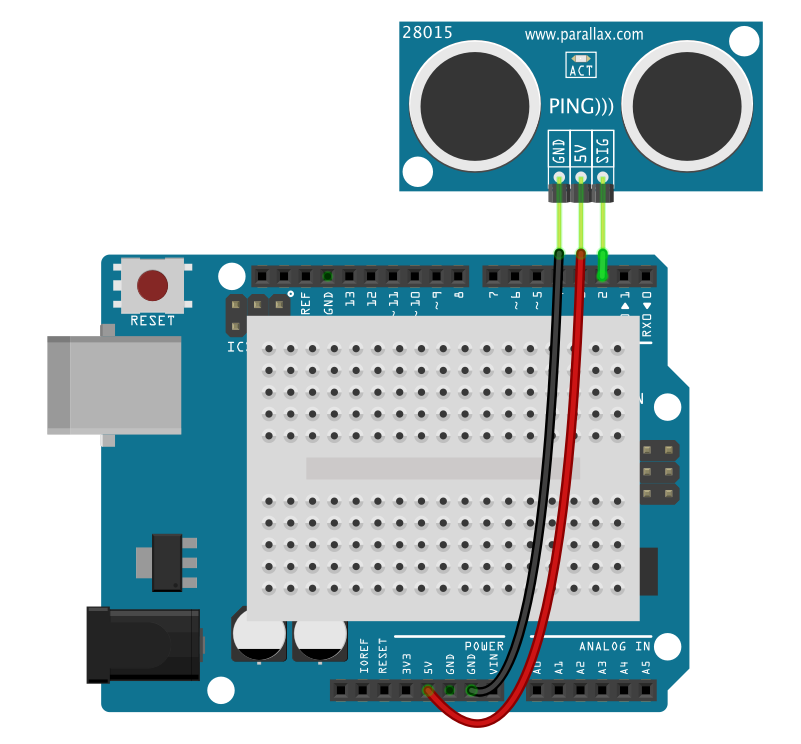
\includegraphics[width=0.5\textwidth]{Kapitel2/Bilder/ping}
\end{multicols}

\section*{Stationskarte: \ref{sec:UmweltSensoren} \nameref{sec:UmweltSensoren}}

\margininfo{}
\begin{multicols}{2}
\subsection*{Material-Liste}
\begin{itemize}
  \item Arduino Uno mit Breadboard
  \item DH11 (Temperatur und Feuchtigkeit)
  \item Widerstand ($10k\Ohm$)
  \item 4 Projekt-Kabel
\end{itemize}

\subsection*{Übersicht Material}

\vfill\null 
\columnbreak

\subsection*{Versuchsaufbau}

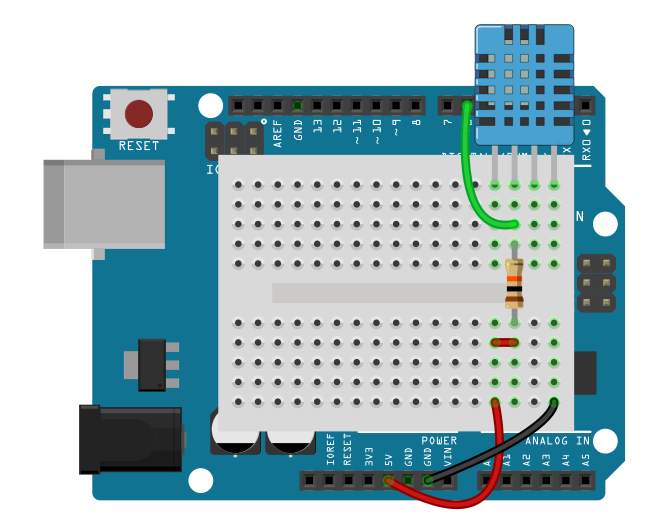
\includegraphics[width=0.5\textwidth]{Kapitel2/Bilder/dh11test}
\end{multicols}




\clearpage 
    \addappheadtotoc
    \appendixpage
    \appendix
    
% Anhang %
\chapter{Hintergrundwissen Arduino}


%%%%%%%%%%%%%%%%%%%%%%%%%%%%%%%%%%%%%%%%%%%%%%%%%%
%% Fehlersuche  %%%%%%%%%%%%%%%%%%%%%%%%%%%%%%%%%%
%%%%%%%%%%%%%%%%%%%%%%%%%%%%%%%%%%%%%%%%%%%%%%%%%%
\section{Fehlersuche}


%%%%%%%%%%%%%%%%%%%%%%%%%%%%%%%%%%%%%%%%%%%%%%%%%%
%% Analoge und digitale Signale %%%%%%%%%%%%%%%%%%
%%%%%%%%%%%%%%%%%%%%%%%%%%%%%%%%%%%%%%%%%%%%%%%%%%
\section{Analoge und digitale Signale}

Ein Analogsignal ist im Rahmen der Signaltheorie eine Form eines Signals mit stufenlosem und unterbrechungsfreiem Verlauf. Ein Analogsignal wird als glatte Funktion beschrieben und es lässt sich damit beispielsweise der zeitlich kontinuierliche Verlauf einer physikalischen Größe wie der Schalldruck in Form eines analogen Audiosignals beschreiben. Der Wertebereich eines Analogsignals wird als Dynamikumfang bezeichnet.

\margininfo{digital von lat. digitus = Finger; mit Fingern wird gezählt}

Ein Digitalsignal  ist eine spezielle Form eines Signals, welches einerseits einen abgegrenzten und gestuften Wertvorrat und zudem in der zeitlichen Abfolge nur zu bestimmten periodischen Zeitpunkten definiert ist bzw. eine Veränderung im Signalwert aufweist. Es kann aus einem Analogsignal, welches den zeitlich kontinuierlichen Verlauf einer physikalischen Größe beschreibt, durch die Quantisierung und eine Abtastung, welche zu definierten Zeitpunkten erfolgt, gebildet werden. Die digitalen Werte sind üblicherweise als Binärzahlen kodiert, so dass ihre Quantisierung in Bits angegeben wird.
\subsection{Digital Analog Wandler}


\subsubsection{Aufbau der Schaltung}

Der Aufbau der Schaltung ist in Abb. und Abb. \ref{fig:8bitDAC} zu sehen. 

In der Abb. \ref{fig:8bitDAC} sind neben dem eigentliche DAC-Wander bestehend aus den neuen $20k\Ohm$ und  sieben $10k\Ohm$ Widerständen ein Potentiometer, das  zur Verändern der Frequenz dient und ein Summer, dessen Aufgabe es ist das Signal akustischen darzustellen.   
  
\marginfigure{Anhang/Bilder/8bitDAC}{8 BIT Analog Digital Wander}{fig:8bitDAC}

\clearpage
\subsubsection{Beispiel-Sketch zum erzeugen eines sinusförmigen Spannungsverlaufes}

\begin{multicols}{2}
\begin{arduinoCode}{Beispielsketch für eine sinusförmigen Spannungsverlauf}{lst:8bitDAC}
int mPoti;

void setup()
{
  for (int i=0;i<8;i++) {
    pinMode(i, OUTPUT); (*@ \tikzmark{pinMode} @*)
  }
}

void loop() {
    mPoti = analogRead(A0);
    
    for (int i=0; i<8;i++) {
      digitalWrite(i, HIGH); 
      delayMicroseconds(mPoti);
      digitalWrite(i, LOW);
    }
 
    for (int i=6;i>0;i--) {
      digitalWrite(i, HIGH);
      delayMicroseconds(mPoti);
      digitalWrite(i, LOW);
    }  
}\end{arduinoCode}

\vfill
\columnbreak

\begin{itemize}
  \itemsep15pt
  \item[] \tikzmarkcomment{item1}{Digital PINs 0 bis 7 werden auf OUTPUT gesetzt}
\end{itemize}


\begin{tikzpicture}[remember picture,overlay]
  \path[red, thick,-] (pinMode.east) edge [out=0 , in=180] (item1);
 \end{tikzpicture}
\vfill 
\end{multicols}


%%%%%%%%%%%%%%%%%%%%%%%%%%%%%%%%%%%%%%%%%%%%%%%%
%% Arduinos Verbindung zur Aussenwelt: PINs %%%%
%%%%%%%%%%%%%%%%%%%%%%%%%%%%%%%%%%%%%%%%%%%%%%%%
\sectionExkurs{Arduino's Verbindung zur Aussenwelt: PINs}

Wie du schon weisst gibt es (neben anderen Anschlüssen) 14 digitale und 6 analoge PINs. In diesem Abschnitt erfährst du wichtiges Hintergrundwissen. Es ist wichtig, dass du diesen Abschnitt aufmerksam liest, da der Inhalt sehr wichtig für dein Verständnis für die Funktionsweise des Arduino-Boards ist. Wenn du mit dem Inhalt noch überfordert bis, kannst du auch zuerst mit Kapitel 2 anfangen, aber du solltest diesen Abschnitt unbedingt lesen und durcharbeiten. Ich habe versucht den Inhalt anhand von Beispielen und Aufgaben aufzulockern. Die Aufgaben sind der Schlüsel zum Verständnis.     

\subsection{Digitale Ein- und Ausgänge} 

Die digitalen PINs des Arduino's können entweder als Ein- oder Ausgänge konfiguriert werden. Du hast beide Arten schon kennengelernt. Im Abschnitt \ref{sec:blink} hast du den digitalen PIN 13 als OUTPUT-PIN  und im Abschnitt \ref{sec:kommunikation} den PIN 02 als INPUT-PIN benutzt.

\subsection{Der INPUT-Mode} 

Die digitalen PINs des Arduino's sind standardmäßig als Eingänge definiert. Es ist also nicht unbedingt nötig (aber trotzdem sinnvoll) sie als Eingänge mit dem Befehl \arduinocode{pinMode(pinNummer,INPUT);} zu definieren. Sinnvoll deswegen, damit deinen Sketch verständlicher wird. Die digitalen PINs haben einen sehr hohe Impedanz.
\margininfo{Impedanz: Die Fähigkeit einen elektrische Ladung lange zu speichern} Dies bedeutet, dass ein kleiner elektrischer Strom ausreicht, damit der PIN seinen Zustand wechselt. Dies kann zum Beispiel für einen kapazitiven Touch-Sensor benutzt werden.

Wenn ein PIN im INPUT-Mode nicht mit einem Sensor verbunden ist, wirkt sich die Hohe Impedanz negativ aus. Wenn du diesen PIN ausliest stellen sich zufällige Ergebnisse für den Zustand an diesem PIN ein! Es findet ein Kopplung mit der in seiner Umgebung vorhandenen Elektrizität statt. Das kann dein Pulli sein, der sich elektrostatisch aufgeladen hat, oder das Laptop. In diesem Fall spricht man davon, dass der Zustand des PINs nicht definiert ist.  

\subsubsection{Aufgabe 1: Ein Touch-Sensor}

Für diese Schaltung benötigt du einen großen Widerstand $(100k\Omega-1M\Omega)$, ein Krokodilklemmen-Kabel und ein Stück Metallfolie. Baue die Schaltung nach Abb. \ref{fig:CapSensor} auf und lade den Beispiel-Sketch aus Listing \ref{lst:CapSensor} auf deinen Arduino. Da die auf dem Arduino-Board am PIN 13 eingebaute LED von dem Projekt-Shield verdeckt wird, kannst du am PIN 13 und GND eine LED einstecken. Wenn du die Schaltung richtig aufgebaut hast, dann sollte die LED an PIN 13 leuchten. Berühre kurz die Metallfolie, dann erlischt die LED für eine Sekunde.   
\marginfigure{Kapitel1/Bilder/CapSensor}{Touchsensor}{fig:CapSensor}


\begin{multicols}{2}
\margininfo{Sollte der Touch-Senor nicht funktionieren, dann könnte es sein, dass du durch den Boden im Schulhaus elektrostatisch aufgeladen bist. Berühre einfach mit der anderen Hand das Gehäuse es USB-Anschlusses, dann sollte der Sensor funktionieren.}

\begin{arduinoCode}{Beispiel-Sketch für einen Touch-Senor}{lst:CapSensor}
const int capPin1 = 7;    (*@ \tikzmark{capPINs} @*) 
const int capPin2 = 8;    
const int ledPin =  13;   
int capState = 0;   (*@ \tikzmark{capState} @*)

void setup() {
  pinMode(ledPin, OUTPUT);  (*@ \tikzmark{pinModes} @*)
  pinMode(capPin1, INPUT);
  pinMode(capPin2, OUTPUT);
}

void loop() {
  capState = digitalRead(capPin1);(*@ \tikzmark{digitalRead} @*)
  digitalWrite(capPin2,HIGH);
  if (capState == HIGH) { (*@ \tikzmark{ifelse} @*)
    digitalWrite(ledPin, HIGH);
  }
  else {
    digitalWrite(ledPin, LOW);
    delay(1000);
  } 
}
\end{arduinoCode}
\vfill
\columnbreak

\null\vfill
\begin{itemize}
  \itemsep15pt
  \item[] \tikzmarkcomment{item1}{Definition der Sensor PINs}
  \item[] \tikzmarkcomment{item2}{Hier soll später der aktuelle Zustand von PIN 7  gespeichert werden.}
  \item[] \tikzmarkcomment{item3}{Deklaration der PINs}
  \item[] \tikzmarkcomment{item4}{Auslesen und speichern des Zustands am PIN 7.}
  \item[] \tikzmarkcomment{item5}{Reaktion auf den gespreicherten Zustand.}
\end{itemize}
\vfill \null

\begin{tikzpicture}[remember picture,overlay]
  \path[red, thick,-] (capPINs.east) edge [out=0 , in=180] (item1);
  \path[red, thick,-] (capState.east) edge [out=0 , in=180] (item2);
  \path[red, thick,-] (pinModes.east) edge [out=0 , in=180] (item3);
  \path[red, thick,-] (digitalRead.east) edge [out=0 , in=180] (item4);
  \path[red, thick,-] (ifelse.east) edge [out=0 , in=180] (item5);
\end{tikzpicture}

\end{multicols}



\subsection{INPUT-Mode und Pullup-Widerstände } 

Im Atmega-Chip sind $20 k\Omega$ Pullup-Widerstände eingebaut, auf die mit Hilfe von Software zugegriffen werden kann. Diese integrierten Pullup-Widerstände werden durch den Arduino-Befehl \arduinocode{pinMode(pinNummer,INPUT)} aktiviert. 

Durch die internen Pullup-Widerstände liegt an einem INPUT-PIN der HIGH-Zustand an. 



Wenn nun ein Sensor mit dem auf INPUT gesetzten digitalen PIN verbunden wird, sollte der andere Ausgang des Sensors mit GND verbunden werden. Im Fall eines einfachen Schalters bewirkt dies, dass wenn der Schalter geschlossen ist der Wert LOW und wenn er geöffnet ist der Wert HIGH am digitalen PIN anliegt.



Oft ist es nützlich, einen digitalen Eingang in einen bekannten Zustand zu steuern, wenn keine Eingabe vorhanden ist. Dies kann mit Hilfe eines Pullup-Widerstand ($+5\V$) oder eines Pulldown-Widerstand (GND) erreicht werden. Pull-Widerstand sollte um die $10k\Ohm$ groß sein. 

\subsubsection{Aufgabe 2}

Ziel dieser Aufgabe ist es das Verhalten eines Pullup- und Pulldown-Widerstandes zu testen. Baue die Schaltung aus Abb. \ref{fig:pull-resistors} auf. Der digitale PIN 03 wird mit einem  $10k\Ohm$-Widerstand mit $+5\V$ verbunden. Der digitale PIN 05 wird mit einem  $10k\Ohm$-Widerstand mit GND verbunden. Mit Hilfe des Sketches \ref{lst:pull-resistors} kannst du den jeweiligen Zustand auslesen. 

\begin{multicols}{2}
\begin{arduinoCode}{Pullup- und Pulldown-Widerstände}{lst:pull-resistors}
int pullDown = 3; (*@ \tikzmark{pullPINs} @*)
int pullUp = 5;

int valuePullDown = 0; (*@ \tikzmark{pinState} @*)
int valuePullUp = 0;

void setup() {
  
  Serial.begin(9600); (*@ \tikzmark{serial} @*)
  
  pinMode(pullDown, OUTPUT); (*@ \tikzmark{pinModes} @*)
  pinMode(pullUp, OUTPUT);
}

void loop() {
  
  valuePullDown = digitalRead(pullDown); (*@ \tikzmark{digitalRead} @*)
  valuePullUp = digitalRead(pullUp);
  
  Serial.print("Wert am PIN 3: ");
  Serial.println(valuePullDown);
  Serial.print("Wert am PIN 5: "); (*@ \tikzmark{printSerial} @*)
  Serial.println(valuePullUp);
  
  delay(200);     
}
\end{arduinoCode}
\vfill
\columnbreak

\null\vfill
\begin{itemize}
  \itemsep15pt
  \item[] \tikzmarkcomment{item1}{Definition der Pull-PINs}
  \item[] \tikzmarkcomment{item2}{Speichern der aktuellen Werte}

  \item[] \tikzmarkcomment{item3}{Starten der seriellen Verbindung}
  \itemsep25pt
  \item[] \tikzmarkcomment{item4}{Deklaration der PINs als OUTPUT, so dass der interne Pulldown-Widerstand nicht verbunden ist.}
  \item[] \tikzmarkcomment{item5}{Auslesen und speichern der Zustände am PIN 3 und 5.}
  \itemsep15pt
  \item[] \tikzmarkcomment{item6}{Ergebnis an PC übertragen.}
\end{itemize}
\vfill \null

\begin{tikzpicture}[remember picture,overlay]
  \path[red, thick,-] (pullPINs.east) edge [out=0 , in=180] (item1);
  \path[red, thick,-] (pinState.east) edge [out=0 , in=180] (item2);
  \path[red, thick,-] (serial.east) edge [out=0 , in=180] (item3);
  \path[red, thick,-] (pinModes.east) edge [out=0 , in=180] (item4);
  \path[red, thick,-] (digitalRead.east) edge [out=0 , in=180] (item5);
  \path[red, thick,-] (printSerial.east) edge [out=0 , in=180] (item6);
\end{tikzpicture}

\end{multicols}
\marginfigure{Kapitel1/Bilder/pull-resistors}{Pullup- und Pulldown-Widerstände}{fig:pull-resistors}

\subsection{PIN 13}

Der digitale PIN 13 ist etwas besonders, da er mit eine LED mit Vorwiderstand verbunden ist. Wenn du diesen PIN auf INPUT setzt, d.h. seinen internen $20k\Ohm$ Pull-up-Widerstand aktivierst, wird das Potenzial bei etwa $1,7\V$ anstatt der erwarteten $5\V$ liegen. Schuld an diesem Umstand ist die LED mit ihrem Vorwiderstand, die die Spannung nach unten ziehen. Das bedeutet, dass dieser PIN immer im Zustand LOW ist! Wenn du den PIN 13 als Eingang verwenden möchtest, musst du den PIN auf INPUT setzen und einen externen Pullup-Widerstand verwenden.



\subsubsection{Aufgabe 3} 
Für diese Aufgabe benötigst du nur das Arduino-Board. Verbinde den analogen PIN A0 mit dem digitalen PIN 13  (siehe Abb. \ref{fig:pin13}). Mit Hilfe des Sketches \ref{lst:pull-resistors} kannst du das Potenzial am PIN 13 messen. 

\marginfigure{Kapitel1/Bilder/pin13}{Potenzial am PIN 13 messen}{fig:pin13}

\begin{multicols}{2}
\begin{arduinoCode}{Verhalten des PINs 13}{lst:pull-resistors}
int pin13 = 13; (*@ \tikzmark{PIN} @*)

int pinPot = 0; (*@ \tikzmark{pinPot} @*)

void setup() {
  
  Serial.begin(9600); (*@ \tikzmark{serial} @*)
  
  pinMode(pin13, INPUT); (*@ \tikzmark{pinModes} @*)
  
}

void loop() {
  
  pinPot = anaolgRead(A0); (*@ \tikzmark{digitalRead} @*)
  
  Serial.print("Potenzial am PIN 13: ");
  Serial.println(pinPot/256); (*@ \tikzmark{printSerial} @*)
  
  delay(200);     
}
\end{arduinoCode}
\vfill
\columnbreak

\null\vfill
\begin{itemize}
  \itemsep15pt
  \item[] \tikzmarkcomment{item1}{Definition der Pull-PINs}
  \item[] \tikzmarkcomment{item2}{Speichern der aktuellen Werte}

  \item[] \tikzmarkcomment{item3}{Starten der seriellen Verbindung}
  \item[] \tikzmarkcomment{item4}{Deklaration der PINs}
  \item[] \tikzmarkcomment{item5}{Auslesen und speichern der Zustände am PIN 3 und 5.}
  \item[] \tikzmarkcomment{item6}{Ergebnis an PC übertragen.}
\end{itemize}
\vfill \null

\begin{tikzpicture}[remember picture,overlay]
  \path[red, thick,-] (PIN.east) edge [out=0 , in=180] (item1);
  \path[red, thick,-] (pinPot.east) edge [out=0 , in=180] (item2);
  \path[red, thick,-] (serial.east) edge [out=0 , in=180] (item3);
  \path[red, thick,-] (pinModes.east) edge [out=0 , in=180] (item4);
  \path[red, thick,-] (digitalRead.east) edge [out=0 , in=180] (item5);
  \path[red, thick,-] (printSerial.east) edge [out=0 , in=180] (item6);
\end{tikzpicture}

\end{multicols}


\subsection{Digitale PINs im OUTPUT Mode} 
Wenn ein digitaler PIN in den Modus OUTPUT gesetzt wird,
ist er in einem niederohmigen Zustand. Dies bedeutet, dass der Arduino sehr leicht kurzgeschlossen werden kann, indem man den PIN direkt mit GND verbindet. Ein digitaler PIN kann maximal bis zu $40\mA$ an Strom für  angeschlossene Geräte liefern. Die maximale Leistung ist groß genug um eine LED die meisten Sensoren zu versorgen, aber nicht groß genug um die Relais, Motoren, Magnetspulen zu betreiben. Diese Bauteile müssen dann mit Hilfe eines Transistor betrieben werden. 

Die digitalen PINs sind sehr empfindlich. Es ist immer eine gute Idee, PINs im OUTPUT Modus mit einem Wiederstand von mind. $220\Ohm$  mit GND zu verbinden.
Gerade bei LEDs sinkt der Widerstand, wenn sie leiten extrem ab. Bei langem Betrieb kann sowohl die LED als auch der digitale PIN verstört werden. 
 
\subsubsection{Aufgabe 4}

Digitale PINs im INPUT Mode liefern sehr wenig Strom, so dass eine LED nur schwach leuchtet. Sollte eine LED nur sehr schwach leuchten dann ist es wahrscheinlich, dass der Mode des PINs falsch gesetzt ist.

Versuche es selbst: Setzte dazu eine rote LED in PIN 13 und GND (schnelle Methode \ref{fig:arduino_blink_schaltung_schnell}) und lade den Sketch aus Listing \ref{lst:inoutled} auf deinen Arduino.  
\begin{multicols}{2}
\begin{arduinoCode}{PIN in input und output Mode}{lst:inoutled}
int ledPin = 13; (*@ \tikzmark{ledPIN} @*)
void setup() {  
}

void loop() {
  pinMode(ledPin, INPUT);
  digitalWrite(ledPin,HIGH); (*@ \tikzmark{input} @*)
  delay(2000);
  
  pinMode(ledPin, OUTPUT);
  digitalWrite(ledPin,HIGH); (*@ \tikzmark{output} @*)
  delay(2000);   
}
\end{arduinoCode}
\vfill
\columnbreak

\null\vfill
\begin{itemize}
  \itemsep15pt
  \item[] \tikzmarkcomment{item1}{Definition des LED-PINs}
  \item[] \tikzmarkcomment{item2}{INPUT-Mode}

  \item[] \tikzmarkcomment{item3}{OUTPUT-Mode}
\end{itemize}
\vfill \null

\begin{tikzpicture}[remember picture,overlay]
  \path[red, thick,-] (ledPIN.east) edge [out=0 , in=180] (item1);
  \path[red, thick,-] (input.east) edge [out=0 , in=180] (item2);
  \path[red, thick,-] (output.east) edge [out=0 , in=180] (item3);
\end{tikzpicture}

\end{multicols}

\subsection{Analoge Input PINs} 

Das Arduino Uno Board hat 6 analoge PINs die mit A0 bis A5 bezeichnet sind. Die Hauptfunktion der analogen PINs ist natürlich das Auslesen von analogen Sensoren. Zusätzlich haben die analogen PINs alle Funktionen der so genannten GPIO-PINs (General Purpose Input/Output), das heißt sie können als zusätzliche digitale PINs verwendet werden.

\subsubsection{Funktionsweise der analogen PINs: A/D-Wandler} 

Der ATmega-IC besitzt einen so genannten integrierte 6-Kanal-Analog-Digital-Wandler (kurz A/D-Wandler). Der A/D-Wandler hat einen Spannungsbereich von $0V$ bis $5\V$, dieser $5\V$ Potenzialunterschied wird in 1024 Teile aufgeteilt was einer Auflösung von 10-Bit ($2^{10} = 1024$) entspricht. 


\begin{table}[h]

\begin{center}

\tikzset{ 
    table/.style={
        matrix of nodes,
        row sep=-\pgflinewidth,
        column sep=-\pgflinewidth,
        nodes={
            rectangle,
            draw=black,
            align=center
        },
        minimum height=1.5em,
        text depth=0.5ex,
        text height=2ex,
        nodes in empty cells,
%%
        every even row/.style={
            nodes={fill=gray!20}
        },
        column 1/.style={
            nodes={text width=0.5\textwidth}
        },
        row 1/.style={
            nodes={
                fill=black!90,
                text=white,
                font=\bfseries
            }
        }
    }
}

\begin{tikzpicture}
\matrix (first) [table,text width=5em]
{   
  $U_{in}$ & 0 & 0.005  & 0.010 & \dots & 4.995 & 5.000 \\
  10-Bit Wert & 0 & 1 & 2 & \dots & 1022 & 1023 \\
};
 \end{tikzpicture}
\end{center}
\caption{Spannung und 10-Bit Wert }
\label{tab:spannung-10-bit}
\end{table}%

Um den Wert der gemessene Spannung auszugeben, muss der gemessene 10-Bit-Wert durch 256 geteilt werden. Dies kann mit Hilfe des Arduino-Befehles map() geschehen:

\subsubsection{Aufgabe 5}
Widerstandsmessung eines unbekannten Widerstandes. Mit Hilfe eines $1k\Ohm$-Widerstandes soll der Wert eines unbekannten Widerstandes bestimmt werden. Dazu müssen die Widerstände in Reihe geschaltet werden. Der unbekannte Widerstand kann dann mit Hilfe der Formel
\begin{eqnarray*}
  R_2 = \frac{U_2}{U_g-U_2}\,R_1
\end{eqnarray*}
berechnet werden. Mit $R_1=1k\Ohm$ und $U_g=5\V$ folgt:
\begin{eqnarray*}
  R_2 = \frac{U_2}{5\V-U_2}\cdot 1k\Ohm
\end{eqnarray*}
 

\marginfigure{Kapitel1/Bilder/widerstandMessung}{Widerstandsmessung}{fig:widerstandMessung}

\begin{multicols}{2}
\null\vfill
\begin{arduinoCode}{Messen eines unbekannten Widerstandes}{lst:widerstandMessung}
float senU = 0.0; (*@ \tikzmark{senU} @*)
float gemR = 0.0;

void setup() {  
  Serial.begin(9600); (*@ \tikzmark{serial} @*)
}

void loop() {
  senU = map(anaolgRead(A0),0,1024,0,5); (*@ \tikzmark{digitalRead} @*)
  
  gemR = senU/(5-senU)*1000;(*@ \tikzmark{rechnung} @*)
    
  Serial.print("R gemessen: ");
  Serial.println(gemR); (*@ \tikzmark{printSerial} @*)
  
  delay(200);     
}
\end{arduinoCode}
\vfill\null 
\columnbreak

\null\vfill
\begin{itemize}
  \itemsep15pt
  \item[] \tikzmarkcomment{item1}{Speichern der aktuellen Werte}

  \item[] \tikzmarkcomment{item2}{Starten der seriellen Verbindung}
  \item[] \tikzmarkcomment{item3}{Messen und umrechnen auf Spannungswert.}
  \item[] \tikzmarkcomment{item4}{Widerstand berechnen}
  \item[] \tikzmarkcomment{item5}{Ergebnis an den PC senden}
\end{itemize}
\vfill \null

\begin{tikzpicture}[remember picture,overlay]
  \path[red, thick,-] (senU.east) edge [out=0 , in=180] (item1);
  \path[red, thick,-] (serial.east) edge [out=0 , in=180] (item2);
   \path[red, thick,-] (digitalRead.east) edge [out=0 , in=180] (item3);
  \path[red, thick,-] (rechnung.east) edge [out=0 , in=180] (item4);
  \path[red, thick,-] (printSerial.east) edge [out=0 , in=180] (item5);
\end{tikzpicture}

\end{multicols}




\subsubsection{Das PIN Mapping}


Analoge PINs können auch als digitale PINs verwendet werden. Um sie von den digitalen PINs unterscheiden zu können, werden die Alias Namen A0 bis A5 verwendet. Um den analogen PIN A0 als digitalen Ausgang mit dem Wert HIGH zu definieren sind folgende Befehle nötig: 
\begin{multicols}{2}
\null\vfill
\begin{arduinoCode}{Analoger PIN wird zum digitalen PIN}{lst:analogPINdigital}
pinMode(A0, OUTPUT); (*@ \tikzmark{output} @*)
digital(A0, HIGH); (*@ \tikzmark{high} @*)
\end{arduinoCode}
\vfill\null 
\columnbreak

\null\vfill
\begin{itemize}
  \itemsep15pt
  \item[] \tikzmarkcomment{item1}{PIN A0 wird zu einem digitalen PIN}
  \item[] \tikzmarkcomment{item2}{A0 wird auf HIGH gesetzt}
\end{itemize}
\vfill \null

\begin{tikzpicture}[remember picture,overlay]
  \path[red, thick,-] (output.east) edge [out=0 , in=180] (item1);
  \path[red, thick,-] (high.east) edge [out=0 , in=180] (item2);
\end{tikzpicture}

\end{multicols}

\subsubsection{Aufgabe 6}
Ändere den Blink Sketch so ab, dass eine LED, die mit dem analogen PIN A0 verbunden ist mit einer Frequenz von einer Sekunde blinkt.

\marginfigure{Kapitel1/Bilder/digitalA0}{Analoger PIN A0 als digitaler PIN verwendet}{fig:digitalA0}

\subsubsection{pullup-Widerstände} 

Die analogen PINs besitzen ebenfalls Pullup-Widerstände. diese Pullup-Widerstände können mit den folgender Befehl aktiviert werden: 
\begin{arduinoCode}{}{}
digital(A0, HIGH); // Set Pullup auf analogen PIN 0 
\end{arduinoCode}
Der PIN sollte natürlich dann im INPUT-Mode sein. 

Das Einschalten des Pullup-Widerstandes verfälscht natürlich die Werte von analogRead()!

\subsubsection{Für Experten!} 

Wenn du die analogen PINs verwenden möchtest, kann es vorkommen, dass sie sich manchmal komisch verhalten.
\begin{itemize}
  \item Wenn ein analoger PIN als Ausgang definiert wurde, wird der Befehl analogRead() nicht korrekt funktionieren. Wenn dies der Fall ist, muss der PIN zuvor als Eingang definiert werden, erst dann kann der Befehl analogRead() korrekt ausgeführt werden. 
 \item  Wenn zwischen verschiedenen analogen Eingang zu schnell gewechselt wird, kann es passieren, dass  A/D-Messwerte durch elektrische Störsignale (genannt Noise) verfälscht werden. Deshalb ist es sinnvoll beim Wechseln von analogen Eingängen eine kurze Pause einzubauen.
\end{itemize}




%%%%%%%%%%%%%%%%%%%%%%%%%%%%%%%%%%%%%%%%%%%%%%%%%%
%% Interruptsteuerung %%%%%%%%%%%%%%%%%%%%%%%%%%%%
%%%%%%%%%%%%%%%%%%%%%%%%%%%%%%%%%%%%%%%%%%%%%%%%%%

\section{Interruptsteuerung}
 
Der Mikrocontroller des Arduino ist mit einer Interrupt-Steuerung (IRC) ausgestattet. Die Aufgabe einer IRC ist es auf stattfindende Ereignisse sofort zu reagieren. Dazu wird die aktuelle Aufgabe unterbrochen und sofort auf das Ereignis zu reagieren.
Man könnten Sie sich fragen, warum ein Interrupt notwendig ist,  um auf externe Ereignisse zu reagieren?
Schließlich können man den Zustand  externer Pins jederzeit überprüfen.

Das Problem ist, dass wenn die Aufgaben komplexer werden, es sicherlich nicht sinnvoll ist alle Abläufe 
in der Loop-Routine abzuarbeiten. Das auf bestimmte Signale unterbrechen der Loop-Routine ist ein
entscheidenden Vorteil - die Unterbrechungen  sind asynchron. 

Ein asynchrones Ereignis ist etwas, das außerhalb des regulären Ablauf der Loop-Routine auftritt -- es
kann jederzeit passieren, egal, was Ihr Sketch im Moment gerade ausführt. Dies bedeutet, dass anstatt 
manuell prüfen, ob ein bestimmtes  Ereignis eintritt, übernimmt diese Aufgabe der Mikrocontroller selbst.

Wenn ein Projekt  ein  genaues Timing verlangt oder schnell auf Eingaben (z.B. von Sensoren) 
reagieren soll,  dann sind Interrupts das Mittel der Wahl. Im folgenden Abschnitt erkläre ich die 
Funktion und Verwendung von Interupts. \citet{engblaze_we_2013}


%Lassen Sie uns ein Beispiel aus der Praxis. Stell dir vor du bist auf der Couch sitzen, genießen einen frostigen brauen und einen Film nach einem langen Tag. Das Leben ist gut. Es gibt nur ein Problem: Sie suchen nach einem unglaublich wichtiges Paket zu kommen warten, und Sie müssen sie so bald wie möglich. Wenn Sie einen normalen AVR-Programm oder Arduino Sketch waren, man müsste wiederholt stilllegen Ihren Film, aufstehen und gehen überprüfen Sie die Mailbox alle 5 Minuten, um sicherzustellen, dass Sie wissen, wann das Paket da war.
%
%Stattdessen vorstellen, wenn das Paket Fedex oder UPS mit Lieferbestätigung versendet. Nun wird die Lieferung Mann bis vor die Haustür und Ring gehen die Türklingel, sobald er ankommt. Das ist Ihre Interrupt auslösen. Sobald Sie den Auslöser, können Sie Pause Ihren Film und gehen viel mit dem Paket. Das ist Ihre Interrupt-Service-Routine. Sobald Sie fertig sind, können Sie abholen den Film wo Sie aufgehört haben, ohne zusätzliche Zeit verschwendet. Das ist die Macht von Interrupts.
%
%Die AVR-Chips in den meisten Arduinos verwendet werden, sind nicht in der Lage parallele Verarbeitung, dh sie können nicht mehrere Dinge auf einmal. Mit asynchrone Verarbeitung über Interrupts ermöglicht es uns, die Effizienz unseres Codes zu maximieren, so dass wir nicht verschwenden keine kostbare Takte am Abfrageschleifen oder warten auf Dinge geschehen. Interrupts sind auch gut für Anwendungen, die präzises Timing erfordern, weil wir wissen, wir fangen unsere Veranstaltung, sobald es auftritt, und nicht versehentlich verpassen.


\subsection{Was sind Interrupts?}

Im Grunde ist ein Interrupt ein Signal, das den ablaufenden Prozess unterbricht. Dieses Signal 
kann entweder durch ein externes Ereignis (z.B. die Änderung eines digitalen Pin Zustandes) oder durch 
ein internes Ereignis (z.B. ein Zeitsignal eines Softwaretimers) ausgelöst werden.

Einmal ausgelöste (triggered), wird ein Interrupt den zur Zeit ablaufenden Prozess anhalten (den 
Zustand dieses Prozesses speichern)  und eine so genannte ``interrupt service routine'' (ISR) 
ausführen. Die ISR reagiert auf den Interrupt, wenn die Abgeschlossen ist, wird er zuvor aufgeführte 
Prozess fortgeführt. 

\begin{figure}[ht]
\begin{center}

% Define a few styles and constants
\tikzstyle{hp}=[draw, fill=blue!20, text width=8em, rounded corners,
    text centered, minimum height=2.5em]
\tikzstyle{irq1} = [hp, fill=red!20]
 
\tikzstyle{pfeil}=[draw,->,black!80,thick,double]
    
\def\blockdist{3.3}
\def\edgedist{2.5}

\begin{tikzpicture}
   \draw[->,thick] (-2,-1) -- (12,-1) node[below=1mm,midway,text width=3cm,text centered] {time};
   \draw[-, thick] (1.7,-1.2) -- (1.7,-0.8)  node[below=1mm,midway,text width=3cm,text centered] {IRQ Signal};
   
   \node (hp1) at (0,0) [hp] {Hauptprozess}; 
   \node (irq) at (5,2.5) [irq1]  {ISR-Routine};  
   \node (hp2) at  (10,0) [hp] {Hauptprozess};
 
    \draw [-to,thick,snake=snake,segment amplitude=.8mm,
         segment length=5mm,line after snake=1mm]
    (hp1.east) -- (irq.west) node [midway] {HP wird unterbrochen};
    \draw [-to,thick,snake=snake,segment amplitude=.8mm,
         segment length=5mm,line after snake=1mm]
    (irq.east) -- (hp2.west) node [midway] {HP wird fortgesetzt};
\end{tikzpicture}
 
\caption{Funktionsweise eines IRQs, das Hauptprogramm wird unterbrochen um die IRQ-Routine auszuführen.}
\label{fig:irq}
\end{center}
\end{figure}



\subsubsection{Die verschiedenen Arten von Interrupts}
Es gibt im Wesentlichen zwei Arten von Interrupts:
\begin{itemize}
\item Hardware-Interrupts, die auf ein externes Ereignis reagieren, wie z. B. wenn bei einem Eingangspin 
der logische Zustand von HIGH nach LOW wechselt.
\item Software-Interrupts, die  auf eine Software Ereignis reagieren.
\end{itemize}
Die 8-bit AVR-Prozessoren,  die meistens in Arduino-Boards verbaut sind, sind  nicht in der Lage auf 
Software-Interrupts zu reagieren.

In  der  Arduino-Sprache  gibt es deshalb nur eine einzige Art von 
Interrupts, die attachInterrupt()-Funktion. 

Für einfache Anwendungen ist diese Funktion ausreichend, aber es gibt noch eine ganz andere Art von
Hardware-Interrupts. 

\subsection{Die Interrupt Service Routines}


Jeder Prozessor AVR hat eine Liste von Interrupt-Quellen, oder Vektoren, die die Art der Ereignisse, die 
einen Alarm auslösen können, umfassen. 
Die Interrupt-Vektor - wenn Interrupts aktiviert sind und eines dieser Ereignisse eintritt, wird der Code an
einer bestimmten Stelle im Programmspeicher springen. Durch das Schreiben eines ISR und dann die 
Anbringung eines Links die es bei der Interrupt-Vektors Speicherplatz, können wir sagen unseren Code, 
um etwas Bestimmtes, wenn ein Alarm ausgelöst wird tun.

Implementieren wir dies mit einem einfachen Beispiel: Erkennen, wann eine Taste gedrückt wurde, und 
eine Aktion auf diesem Pressefreiheit. In diesem Tutorial verwenden wir ein Standard Arduino-Board, um 
die Dinge konsequent, wenn wir uns auf die Pins und unser Programm Setup beziehen. Sie können 
diese Techniken mit einem einfachen AVR zu nutzen, brauchen Sie nur auf das Datenblatt überprüfen, 
um sicherzustellen, dass Sie wissen, welche Pins die Sie benötigen. Hier ist unser Beispiel Schaltung:

\subsubsection{Die Arduino Interrupt-Funktion}

\subsubsection{Implementierung eines Interrupt in einem  Sketch}


%\subsection{AVR und Arduino timer interrupts}
%
%\subsubsection{Was ist ein timer?}
%\subsubsection{Wie arbeiten timer?}
%\subsubsection{Verschiedene Arten von timers}
%\subsubsection{Konfiguration und Ausführen eines timers}
%\subsubsection{Timer prescaling and CTC}



\chapter{Data Kommunikations Systeme}
%%%%%%%%%%%%%%%%%%%%%%%%%%%%%%%%%%%%%%%%%%%%%%%%%%
%% Serielle Schnittstelle %%%%%%%%%%%%%%%%%%%%%%%%
%%%%%%%%%%%%%%%%%%%%%%%%%%%%%%%%%%%%%%%%%%%%%%%%%%
\section{Serielle Schnittstelle - die Verbindung mit dem PC}

Die verschiedenen Komponenten eines Computersystems müssen Informationen austauschen, dieser Austausch vollzieht sich mit Hilfe von Schnittstellen. Es macht sinn, für diese Schnittstellen bestimmte Konventionen festzulegen und einzuhalten, damit die Datenkommunikation reibungslos ablaufen kann. Eine mögliche Schnittstelle ist die sog. serieller Schnittstelle.

\subsection{Die TTY-Schnittstelle} 
Die TTY-Schnittstelle ist die älteste serielle Schnittstelle und wurde ursprünglich zur Verbindung von Fernschreibern entwickelt.  Da im Ruhezustand ein konstanter Gleichstrom von 20 mA fließt, wird die Schnittstelle oft auch als 20-mA-Stromschnittstelle bezeichnet.
\margininfo{Der Optokoppler dient zur galvanische Trennung von Sender- und Empfänger-Stromkreis.}
\begin{figure}[htbp]
  \begin{center}
  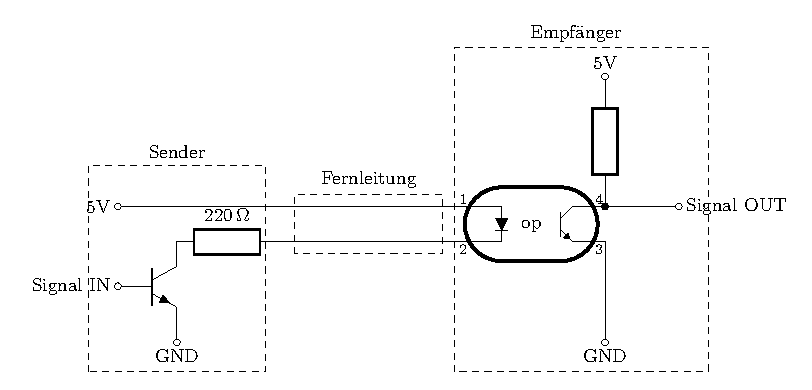
\includegraphics[width=0.8\textwidth]{Anhang/Tikz/tty-schaltung.pdf}
  \caption{TTY Schaltung (nur eine Richtung)}
  \label{fig:ttySchaltung}  
  \end{center}
\end{figure}
Die Übertragung von Daten geschieht nun einfach so, dass der Sender den Schleifenstrom in einem bestimmten Rhythmus unterbricht. Der Empfänger erkennt die rhythmischen Unterbrechungen. Für diese Art der Datenübertragung genügt eine 2-adrigen Leitung ohne. Die Datenübertragung funktioniert aber immer nur ein eine Richtung. Für den gleichzeitigen Datenversand benötigt man getrennte Stromschleifen für Senden und Empfang. Heute wird die TTY-Schnittstelle mit moderne Halbleiterbauelemente realisiert. Der Strom wird mit Hilfe eines Schalttransistor modelliert, der Empfang der Daten durch einen Optokoppler (siehe Abb. \ref{fig:ttySchaltung}).

\subsection{Aufbau eines seriellen Datenpakets}
Auf der Leitung liegt zu jedem Zeitpunkt nur ein BIT (siehe Abb. \ref{fig:serialDaten}). 
Die zu übertragende Daten werden in einzelnen Datenpakete aufgeteilt. Ein Datenpaket besteht aus 7-Daten-BITs und 3 Steuerung-BITs.

\begin{figure}[htbp]
  \begin{center}
      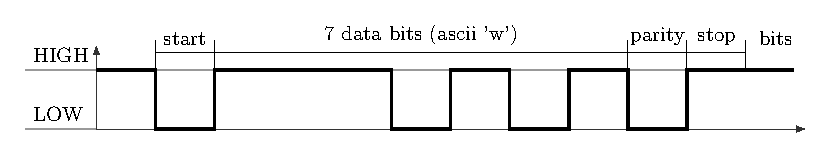
\includegraphics{Anhang/Tikz/serialDaten.pdf}
  \end{center}
  \label{fig:serialDaten}
  \caption{Serielles Datenpaket (das 7-BIT ASCII-Zeichen 'w' wird übertragen)}
\end{figure}

Jedes Datenpaket beginnt mit dem start-BIT (log. LOW). Danach folgen die chrakter-BITs die zu sendenden Daten (z.B. sieben Bit des ASCII-Codes). Als Abschluss folgt das paritäts-BIT und ein oder zwei stop-BITs (log. HIGH), worauf die Leitung wieder im Ruhezustand (log. HIGH) ist. 

Jedes BIT liegt für die gleiche, feste Zeitspanne auf der Leitung. Die Übertragungsgeschwindigkeit wird in Boud angegeben. \margininfo{Die Firma Baudot, eine Pionier der Fernschreibertechnik war Namensgeber für die Einheit Boud \\ 1 Baud = 1 Bit pro Sekunde.} 
Denn zwischen einzelnen Datenpaketen die Leitung beliebig lange im Ruhezustand verharren kann, ist die maximale Übertragungsgeschwindigkeit erreicht, wenn die Datenpakete, direkt aufeinaderfolgen. Wenn zum Beispiel einzelne 7-Bit-ASCII-Zeichen übertragen werden, so ergibt sich bei 9600 Baud eine maximale Datenrate von $ 9600/(7+3) = 960 $ Zeichen pro Sekunde. 

Damit der Empfänger ein Datenpaket empfangen kann muss er zum einen den Anfang und das Ende des Datenpakets erkennen. Zusätzlich zu den Datenbits kann ein sog. Paritäts-BIT übertragen werden mit dessen Hilfe der  Empfänger Übertragungsfehler erkennen kann.  

\subsubsection{start-BIT}
Jeden Datenpaket wird durch das Start BIT eingeleitet. Werden keine Daten übertragen, befindet sich die Leitung im Ruhezustand (log. HIGH). Das Start BIT setzt die Leitung für die Dauer eines BITs auf log. LOW. Der Empfänder weiss nun, dass die folgenden 7 BITs die Daten enthalten.


\subsubsection{parity-BIT}
Das Parität BIT ermöglicht eine primitive Fehlerkontrolle. Wird mit gerader Parität gearbeitet, so setzt der Sender das Paritätsbit auf log. HIGH, falls die Daten-BITs eine ungerade Anzahl von gesetzten (log. HIGH) BITs enthält. Bei einer geraden Anzahl wird das Paritätsbit auf log. LOW gesetzt. Der Empfänger prüft nun nach der gleichen Vorschrift, ob das Paritätsbit zu den Datenbits 'passt'. Falls bei der Übertragung eines der Datenbits verfälscht worden ist, so ist dies also vom Empfänger erkennbar. Wenn zwei Übertragungsfehler vorliegen, dann kann der Empfänger das nicht mehr erkenne.


\subsubsection{stop-BIT}

Das stop-BIT (log. LOW) beendet das Datenpaket. Danach geht die Datenleitung in den Ruhezustand (log. HIGH) über. Dieser Ruhezustand besteht bis zum nächsten Start BIT   


\subsection{RS-232: eine moderne serielle Schnittstelle}
Die RS-232-Schnittstelle wurde ursprünglich bei Großcomputern verwendet, um Terminals an einen Zentralrechner anzuschließen. 
 \marginfigure{Anhang/Tikz/serial-schnittstellen.pdf}{tx und rx PINs auf dem Arduino Board}{fig:serial-schnittstellen}
Sie wurde bis zur Einführung der USB-Schnittstelle auch zum Anschluß von Peripheriegeräten (zum Drucker, Modem etc) an einen Rechner benutzt. Bei technischen Anwendungen, wie zum Beispiel CNC-Maschinen wird die serielle Schnittstelle heute immer noch verwendet. Physikalisch ist die RS-232-Schnittstelle eine Spannungsschnittstelle für jede Richtung ist eine Signalader erforderlich, dazu kommt eine gemeinsame GND-Leitung. \margininfo{Der PIN zum Senden von Daten wird tx (transmit) und zum empfangen von Daten rx (recieve) genannt.} 


\subsection{UART serieller Interface-IC}
Prinzipiell kann man das serielle Datenpaket softwaretechnisch erzeugen, indem man eine digitalen PIN  zu den richtigen Zeitpunkten auf LOW oder HIGH setzt. Der Datenempfang per Software ist schon etwas schwieriger zu bewältigen. In der Praxis verwendet man meist einen seriellen Interface-IC, UART \margininfo{UART steht für Universal Asynchronous Receiver and Transmitter}  genannt. Das Arduino Board besitzt einen UART-Port, dieser kann mit Hilfe der System-Bibliothek Serial gesteuert werden. 

\subsection{Softwaretechnisch Daten von Arduino zu Arduino senden}
Obwohl es für das senden von Daten über eine serielle Schnittstelle die Systembibliothek Serial gibt, mach es Sinn sich die ganze Sache genauer anzuschauen und selber eine Softwarelösung zu programmieren.
 
\subsubsection{Aufbau der Schaltung}
Für den Aufbau einer seriellen Verbindung unter zwei Arduinos müssen nur zwei digtiale PINs und zwei GND PINs miteinander verbunden werden.
\begin{figure}[h]
  \begin{center}
    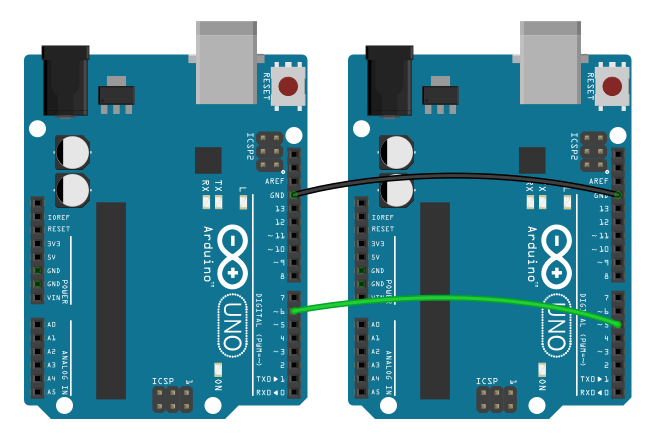
\includegraphics[width=0.6\textwidth]{Anhang/Bilder/arduino-to-arduino.png}
  \end{center}
  \label{fig:arduino-to-arduino}
  \caption{Arduino zu Arduino Verbindung mit einer seriellen Schnittstelle}
\end{figure}
  
\subsubsection{Das Senden von Daten}

\begin{multicols}{2}
\begin{arduinoCode}{}{}
#include <ctype.h>
#define bit9600Delay 84 (*@ \tikzmark{delay} @*)  

byte tx = 6;

void setup() {
  pinMode(tx,OUTPUT);
  digitalWrite(tx,HIGH);
}

void SWprint(int data)
{
  byte mask;
  digitalWrite(tx,LOW); (*@ \tikzmark{startBit} @*)
  delayMicroseconds(bit9600Delay); 
  for (mask = 0x01; mask>0; mask <<= 1) {
    if (data & mask){ // choose bit
     digitalWrite(tx,HIGH); (*@ \tikzmark{highBit} @*)
    }
    else{
     digitalWrite(tx,LOW); (*@ \tikzmark{lowBit} @*)
    }
    delayMicroseconds(bit9600Delay);
  }
  digitalWrite(tx, HIGH); (*@ \tikzmark{stopBit} @*)
  delayMicroseconds(bit9600Delay);  
 
}

void loop()
{
    SWprint(toupper('w'));      
}
\end{arduinoCode}

\vfill
\columnbreak

\begin{itemize}
  \itemsep15pt
  \item[] \tikzmarkcomment{item1}{Initialisieren der Schleifenvariablen}
\end{itemize}


\begin{tikzpicture}[remember picture,overlay]
  \path[red, thick,-] (delay.east) edge [out=0 , in=180] (item1);
 \end{tikzpicture}
\vfill 
\end{multicols}

\subsubsection{Das Empfangen von Daten}

\begin{multicols}{2}
\begin{arduinoCode}{}{}
#include <ctype.h>
#define bit9600Delay 84 (*@ \tikzmark{delay} @*)  

byte rx = 5;
byte SWval;

void setup() {
  pinMode(rx,INPUT);
}

int SWread() {
  byte val = 0;
  while (digitalRead(rx));
  if (digitalRead(rx) == LOW) {
    delayMicroseconds(halfBit9600Delay);
    for (int offset = 0; offset < 8; offset++) {
     delayMicroseconds(bit9600Delay);
     val |= digitalRead(rx) << offset;
    }
    delayMicroseconds(bit9600Delay); 
    delayMicroseconds(bit9600Delay);
    return val;
  }
}

void loop()
{
    SWval = SWread(); 
}
\end{arduinoCode}

\vfill
\columnbreak

\begin{itemize}
  \itemsep15pt
  \item[] \tikzmarkcomment{item1}{Initialisieren der Schleifenvariablen}
\end{itemize}


\begin{tikzpicture}[remember picture,overlay]
  \path[red, thick,-] (delay.east) edge [out=0 , in=180] (item1);
 \end{tikzpicture}
\vfill 
\end{multicols}

\subsubsection{Ergebnis}

\begin{figure}[htbp]
  \begin{center}
    \subfigure[]{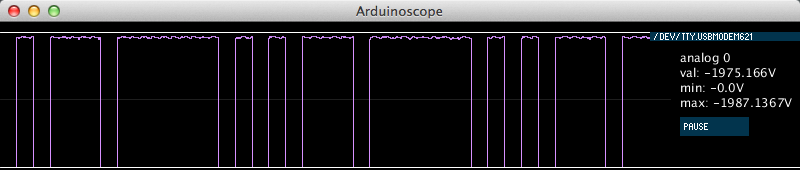
\includegraphics[width=0.7\textwidth]{Anhang/Bilder/serialW.png}}
    \subfigure[]{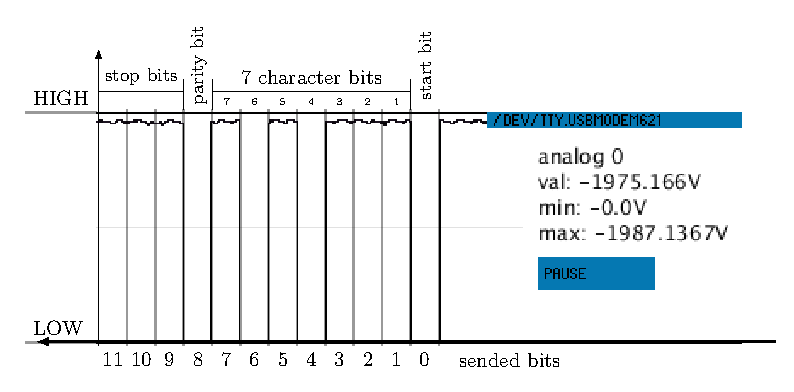
\includegraphics[width=0.6\textwidth]{Anhang/Tikz/serial-wo.pdf}}
  \end{center}
  \label{fig:serialW}
  \caption{Serielles Signal}
\end{figure}

\section{I2C Schnittstelle}

Der I2C Bus ist ein synchroner serieller 2-Draht Bus, der in den 80er Jahren von Philips entwickelt wurde. I2C gesprochen 'I Quadrat C' kommt von der der Abkürzung IIC und bedeutet Inter-Integrated Circuit. Er wird hauptsachlich dazu benutzt, zwischen Schaltkreisen, die sich auf einer Platine verbinden, Daten auszutauschen. Die beiden Leitungen, die den I2C Bus bilden heißen SCL und SDA. SCL steht für Signal Clock und ist die Taktleitung für den Bus. Deshalb spricht man auch von einem synchronen Bus. SDA steht für Signal Data und ist die Datenleitung. Die Datenübertragungsrate des I2C Busses beträgt 100kHz im Standard Mode, bzw. 400kHz im Fast Mode. Aus Lizenzgründen nennt man das I2C Interface bei Atmel TWI (Two Wire Interface).

Der I2C Bus ist ein Multi Master/Slave Bus. Das bedeutet, es gibt mindestens einen I2C Master und ebenso mindestens einen I2C Slave. Der Master selektiert einen Slave durch seine Slave Adresse, die innerhalb eines Busses eindeutig sein muss. Eine Datenübertragung kann nur durch einen I2C Master initiiert werden. Der Slave bleibt immer passiv und lauscht nur auf die Slave Adresse und vergleicht diese mit seiner eigenen Slave Adresse. Erst wenn er seine Slave Adresse erkennt, greift der Slave auch aktiv in das Busgeschehen ein.

Aus Sicht des I2C Masters unterscheidet man zwischen Read und Write Sequenzen. Bei einer Read Sequenz liest der I2C Master Daten vom I2C Slave. Bei einer Write Sequenz sendet der I2C Master Daten zum Slave.



\chapter{Hintergrundwissen: Programmieren}

\section{Rechnen im dem Mikrocontroller}

\section{Programmablaufplan }

\chapter{Hintergrundwissen: Elektronik} \label{ch:anhang_elektronik}

\section{Multimeter}

\begin{multicols}{2}
\begin{tikzpicture}
  % grid 
  \draw[color=red,help lines,xstep=1,ystep=1] (0,0) grid (6,10);
  \draw[help lines,thin,xstep=.5,ystep=.5] (0,0) grid (7,10);
  \foreach \x in {0,1,...,7} { \node [anchor=north] at (\x,0) {\x}; }
  \foreach \y in {0,1,...,10} { \node [anchor=east] at (0,\y) {\y}; }
  % Image
  \node[anchor=south west,inner sep=0] (image) at (0,0) {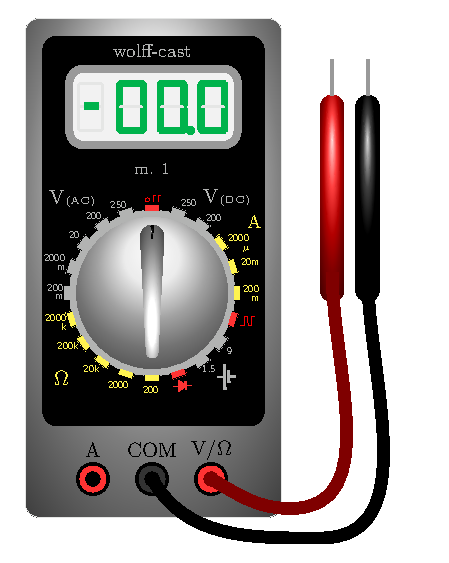
\includegraphics{Anhang/Tikz/multimeter.pdf}};
  % Marks 
  \node[] at (4,8) {\tikzmark{lcd}};
  \node[] at (2.8,4) {\tikzmark{wire}};
  \node[] at (2.05,3.4) {\tikzmark{crystal}};
  \node[] at (2.6,0.5) {\tikzmark{anode}};
  \node[] at (1.4,-0.5) {\tikzmark{cathode}};
  cathode
\end{tikzpicture}

\columnbreak
\vfill\null 
\begin{itemize}
  \itemsep20pt
    \item[] \tikzmarkcomment{item1}{4 stellige LCD-Anzeige}
    \item[] \tikzmarkcomment{item2}{Anschlussdraht für den Halbleiterkristall aus Gold}
    \item[] \tikzmarkcomment{item3}{Halbleiterkristall in Reflektorwanne}
    \item[] \tikzmarkcomment{item4}{Anode der LED (Langer PIN)}
    \item[] \tikzmarkcomment{item5}{Kathode der LED (Kurzer PIN)}
 \end{itemize}
\vfill \null

\begin{tikzpicture}[remember picture,overlay]
  \path[red, thick,-] (lcd.east) edge [out=0 , in=180] (item1);
  \path[red, thick,-] (wire.east) edge [out=0 , in=180] (item2);
  \path[red, thick,-] (crystal.east) edge [out=0 , in=180] (item3);
  \path[red, thick,-] (anode.east) edge [out=0 , in=180] (item4);
  \path[red, thick,-] (cathode.east) edge [out=0 , in=180] (item5);
\end{tikzpicture}
\end{multicols}


\section{Farbcodes von Widerständen} 

Auf Schichtwiderstände  werden die Widerstandswerte  mit Hilfe von farbigen Ringen aufgemalt. Dies hat gegen¸ber Aufschriften den Vorteil, dass die Kennzeichnung eines in eine Schaltung eingelˆteten Widerstandes auf jeden Fall zu erkennen ist. Um den Widerstandswert bestimmen zu kˆnnen, braucht man den Farbcode. Bei einem Widerstand mit vier Ringen geben die ersten beiden Ringe die Zahlen vor der Zehnerpotenz an. Die Farbe des dritten Rings gibt den Exponenten der Zehnerpotenz an. Der vierte, etwas abgesetzte Ring macht eine Angabe ¸ber die Toleranz des Widerstandswertes. Fehlt der Toleranzring, so kann man davon ausgehen, dass der Widerstandswert nur auf $\pm20\%$ genau ist.
\begin{table}[h]

\begin{center}
\begin{tabular}{|p{0.2\textwidth}|c|c|c|c|}\hline 
\rowcolor{lightgray} Ringfarbe      & \multicolumn{4}{c|}{Ring Nr. 1 -- 4 } \\\hline 
Silber  \cellcolor{silver}    & -- & -- & $10^{-2}$  &  $\pm10$\%\\\hline
Gold    \cellcolor{gold}    & -- & -- &  $10^{-1}$ &  $\pm5$\%\\\hline
\textcolor{white}{Schwarz}  \cellcolor{black}& -- & 0 & $10^{0}$   &  --  \\\hline
Braun   \cellcolor{brown}   & 1 & 1 & $10$            &  $\pm1$\%\\\hline
Rot    \cellcolor{red}      & 2 & 2 & $10^{2}$    &  $\pm2$\%\\\hline
Orange   \cellcolor{orange}& 3 & 3 & $10^{3}$    &  --\\\hline
Gelb      \cellcolor{yellow} & 4  & 4 & $10^{4}$ &  \\\hline
Gr¸n      \cellcolor{green} & 5  & 5 & $10^{5}$ &  $\pm0.5$\%\\\hline
Blau       \cellcolor{blue} & 6  & 6 & $10^{6}$ &  $\pm0.25$\%\\\hline
Lila         \cellcolor{violet} & 7  & 7 & $10^{7}$ &  $\pm0.1$\%\\\hline
Grau        \cellcolor{gray}  & 8  & 8 & --              &  $\pm0.05$\%\\\hline
Weiß       & 9  & 9 & --              &  -- \\\hline
\end{tabular}
\end{center}
\caption{Farbkodes von Kohleschichtwiderständen}
\label{tab:farbcodes}
\end{table}%

\textbf{Aufgabe:} Bestimme die Widerstandswerte folgender Widerstände. \\[0.2cm]
\begin{minipage}{0.3\textwidth}
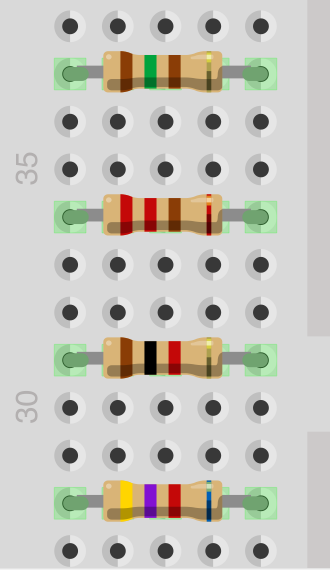
\includegraphics[width=0.8\textwidth]{Anhang/Bilder/widerstaede}
\end{minipage}
\begin{minipage}{0.7\textwidth}
\begin{itemize}
\item[a)] 
\begin{tabular}{|p{0.15\textwidth}|p{0.1\textwidth}|p{0.1\textwidth}|p{0.1\textwidth}|p{0.1\textwidth}|p{0.2\textwidth}|}\hline 
\rowcolor{lightgray} Ring Nr.      & 1 & 2 & 3 & 4  & Ergebnis \\\hline 
Farbe   & braun & rot &  braun & gold & -- \\\hline
Wert     &  1        & 5    & $\cdot 10$ & $\pm 20\%$ & $150\pm20\%\Omega$ \\\hline 
\end{tabular}
\item[b)]
\begin{tabular}{|p{0.15\textwidth}|p{0.1\textwidth}|p{0.1\textwidth}|p{0.1\textwidth}|p{0.1\textwidth}|p{0.2\textwidth}|}\hline 
\rowcolor{lightgray} Ring Nr.      & 1 & 2 & 3 & 4  & Ergebnis \\\hline 
Farbe   &  \qquad& \qquad&  \qquad & \qquad & -- \\\hline
Wert     &          &    & & & \\\hline
\end{tabular}

\item[c)]
\begin{tabular}{|p{0.15\textwidth}|p{0.1\textwidth}|p{0.1\textwidth}|p{0.1\textwidth}|p{0.1\textwidth}|p{0.2\textwidth}|}\hline 
\rowcolor{lightgray} Ring Nr.      & 1 & 2 & 3 & 4  & Ergebnis \\\hline 
Farbe   &  \qquad& \qquad&  \qquad & \qquad & -- \\\hline
Wert     &          &    & & & \\\hline
\end{tabular}

\item[d)]
\begin{tabular}{|p{0.15\textwidth}|p{0.1\textwidth}|p{0.1\textwidth}|p{0.1\textwidth}|p{0.1\textwidth}|p{0.2\textwidth}|}\hline 
\rowcolor{lightgray} Ring Nr.      & 1 & 2 & 3 & 4  & Ergebnis \\\hline 
Farbe   &  \qquad& \qquad&  \qquad & \qquad & -- \\\hline
Wert     &          &    & & & \\\hline
\end{tabular}

\end{itemize}

\end{minipage}


%%%%%%%%%%%%%%%%%%%%%%%%%%%%%%%%%%%%%%%%%%%%%%%%%%%%%%
%%%%%% Hintergrundswissen LED %%%%%%%%%%%%%%%%%%%%%%%%%
%%%%%%%%%%%%%%%%%%%%%%%%%%%%%%%%%%%%%%%%%%%%%%%%%%%%%%
\section{Hintergrundwissen LED}
\label{sec:led}

\subsection{Funktionsweise}


\begin{multicols}{2}
\begin{tikzpicture}
  % grid 
  %\draw[help lines,xstep=1,ystep=1] (0,0) grid (4,7);
  %\draw[help lines,thin,xstep=.2,ystep=.2] (0,0) grid (4,7);
  %\foreach \x in {0,1,...,4} { \node [anchor=north] at (\x,0) {\x}; }
  %\foreach \y in {0,1,...,7} { \node [anchor=east] at (0,\y) {\y}; }
  % Image
  \node[anchor=south west,inner sep=0] (image) at (0,-3.5) {\includegraphics{Anhang/Tikz/ledFkt.pdf}};
  % Marks 
  \node[] at (2.7,6) {\tikzmark{lens}};
  \node[] at (2.8,4) {\tikzmark{wire}};
  \node[] at (2.05,3.4) {\tikzmark{crystal}};
  \node[] at (2.6,0.5) {\tikzmark{anode}};
  \node[] at (1.4,-0.5) {\tikzmark{cathode}};
  cathode
\end{tikzpicture}

\columnbreak
\vfill\null 
\begin{itemize}
  \itemsep20pt
    \item[] \tikzmarkcomment{item1}{Gehäuse das als Linse dient aus Epoxidharz}
    \item[] \tikzmarkcomment{item2}{Anschlussdraht für den Halbleiterkristall aus Gold}
    \item[] \tikzmarkcomment{item3}{Halbleiterkristall in Reflektorwanne}
    \item[] \tikzmarkcomment{item4}{Anode der LED (Langer PIN)}
    \item[] \tikzmarkcomment{item5}{Kathode der LED (Kurzer PIN)}
 \end{itemize}
\vfill \null

\begin{tikzpicture}[remember picture,overlay]
  \path[red, thick,-] (lens.east) edge [out=0 , in=180] (item1);
  \path[red, thick,-] (wire.east) edge [out=0 , in=180] (item2);
  \path[red, thick,-] (crystal.east) edge [out=0 , in=180] (item3);
  \path[red, thick,-] (anode.east) edge [out=0 , in=180] (item4);
  \path[red, thick,-] (cathode.east) edge [out=0 , in=180] (item5);
\end{tikzpicture}
\end{multicols}

\subsection{Vorwiderstand einer LED berechenen}


\section{Schaltungsentwicklung mit Fritzing}


\chapter{Hintergrundwissen: Free Software Foundation and Creative Commons}

\section{Open Source und Creative Commons}





% Literaturliste soll im Inhaltsverzeichnis auftauchen
\newpage
\addcontentsline{toc}{section}{Literatur}

% Literaturliste endgueltig anzeigen
\bibliography{Arduino}


\printindex


\end{document}


